\chapter{Flow Control}
In this chapter, implementation and evaluation of various control algorithms for flow control purposes will be presented. At first, the aim is to enable regulation of flow to a constant value. Later on, the system's ability to follow different reference flow trajectories will be tested. In a final step, the system will be subjected to disturbances through the HiL test rig in form of heart beats at different heart rates. Performances of the implemented control algorithms will be compared.
% As a first step towards flow control implementation two versions of PI controllers are implemented to ensure stable system behavior. After comparing the performance results of both approaches, a parallel approach to ILC implementation under use of the higher performing PI controller is applied to improve the follow up behavior and reduce control errors.
\section{PI Controller}
PI control implementation is performed on the basis of the tuning rules according to Ziegler Nichols as well as according to Chien Hrones Reswick (Chapter \ref{chap:CHR}). The performance of both controllers later on is  compared and evaluated.
\subsection{Design and Implementation}
As a preparation for utilization of the inflection tangent method for these tuning approaches, a measurement similar to the one for determining the static map is performed. \figurename~\ref{fig:dyn_meas} depicts the signal curves for determination of the tuning parameters.
\begin{figure}[ht]
  \centering
  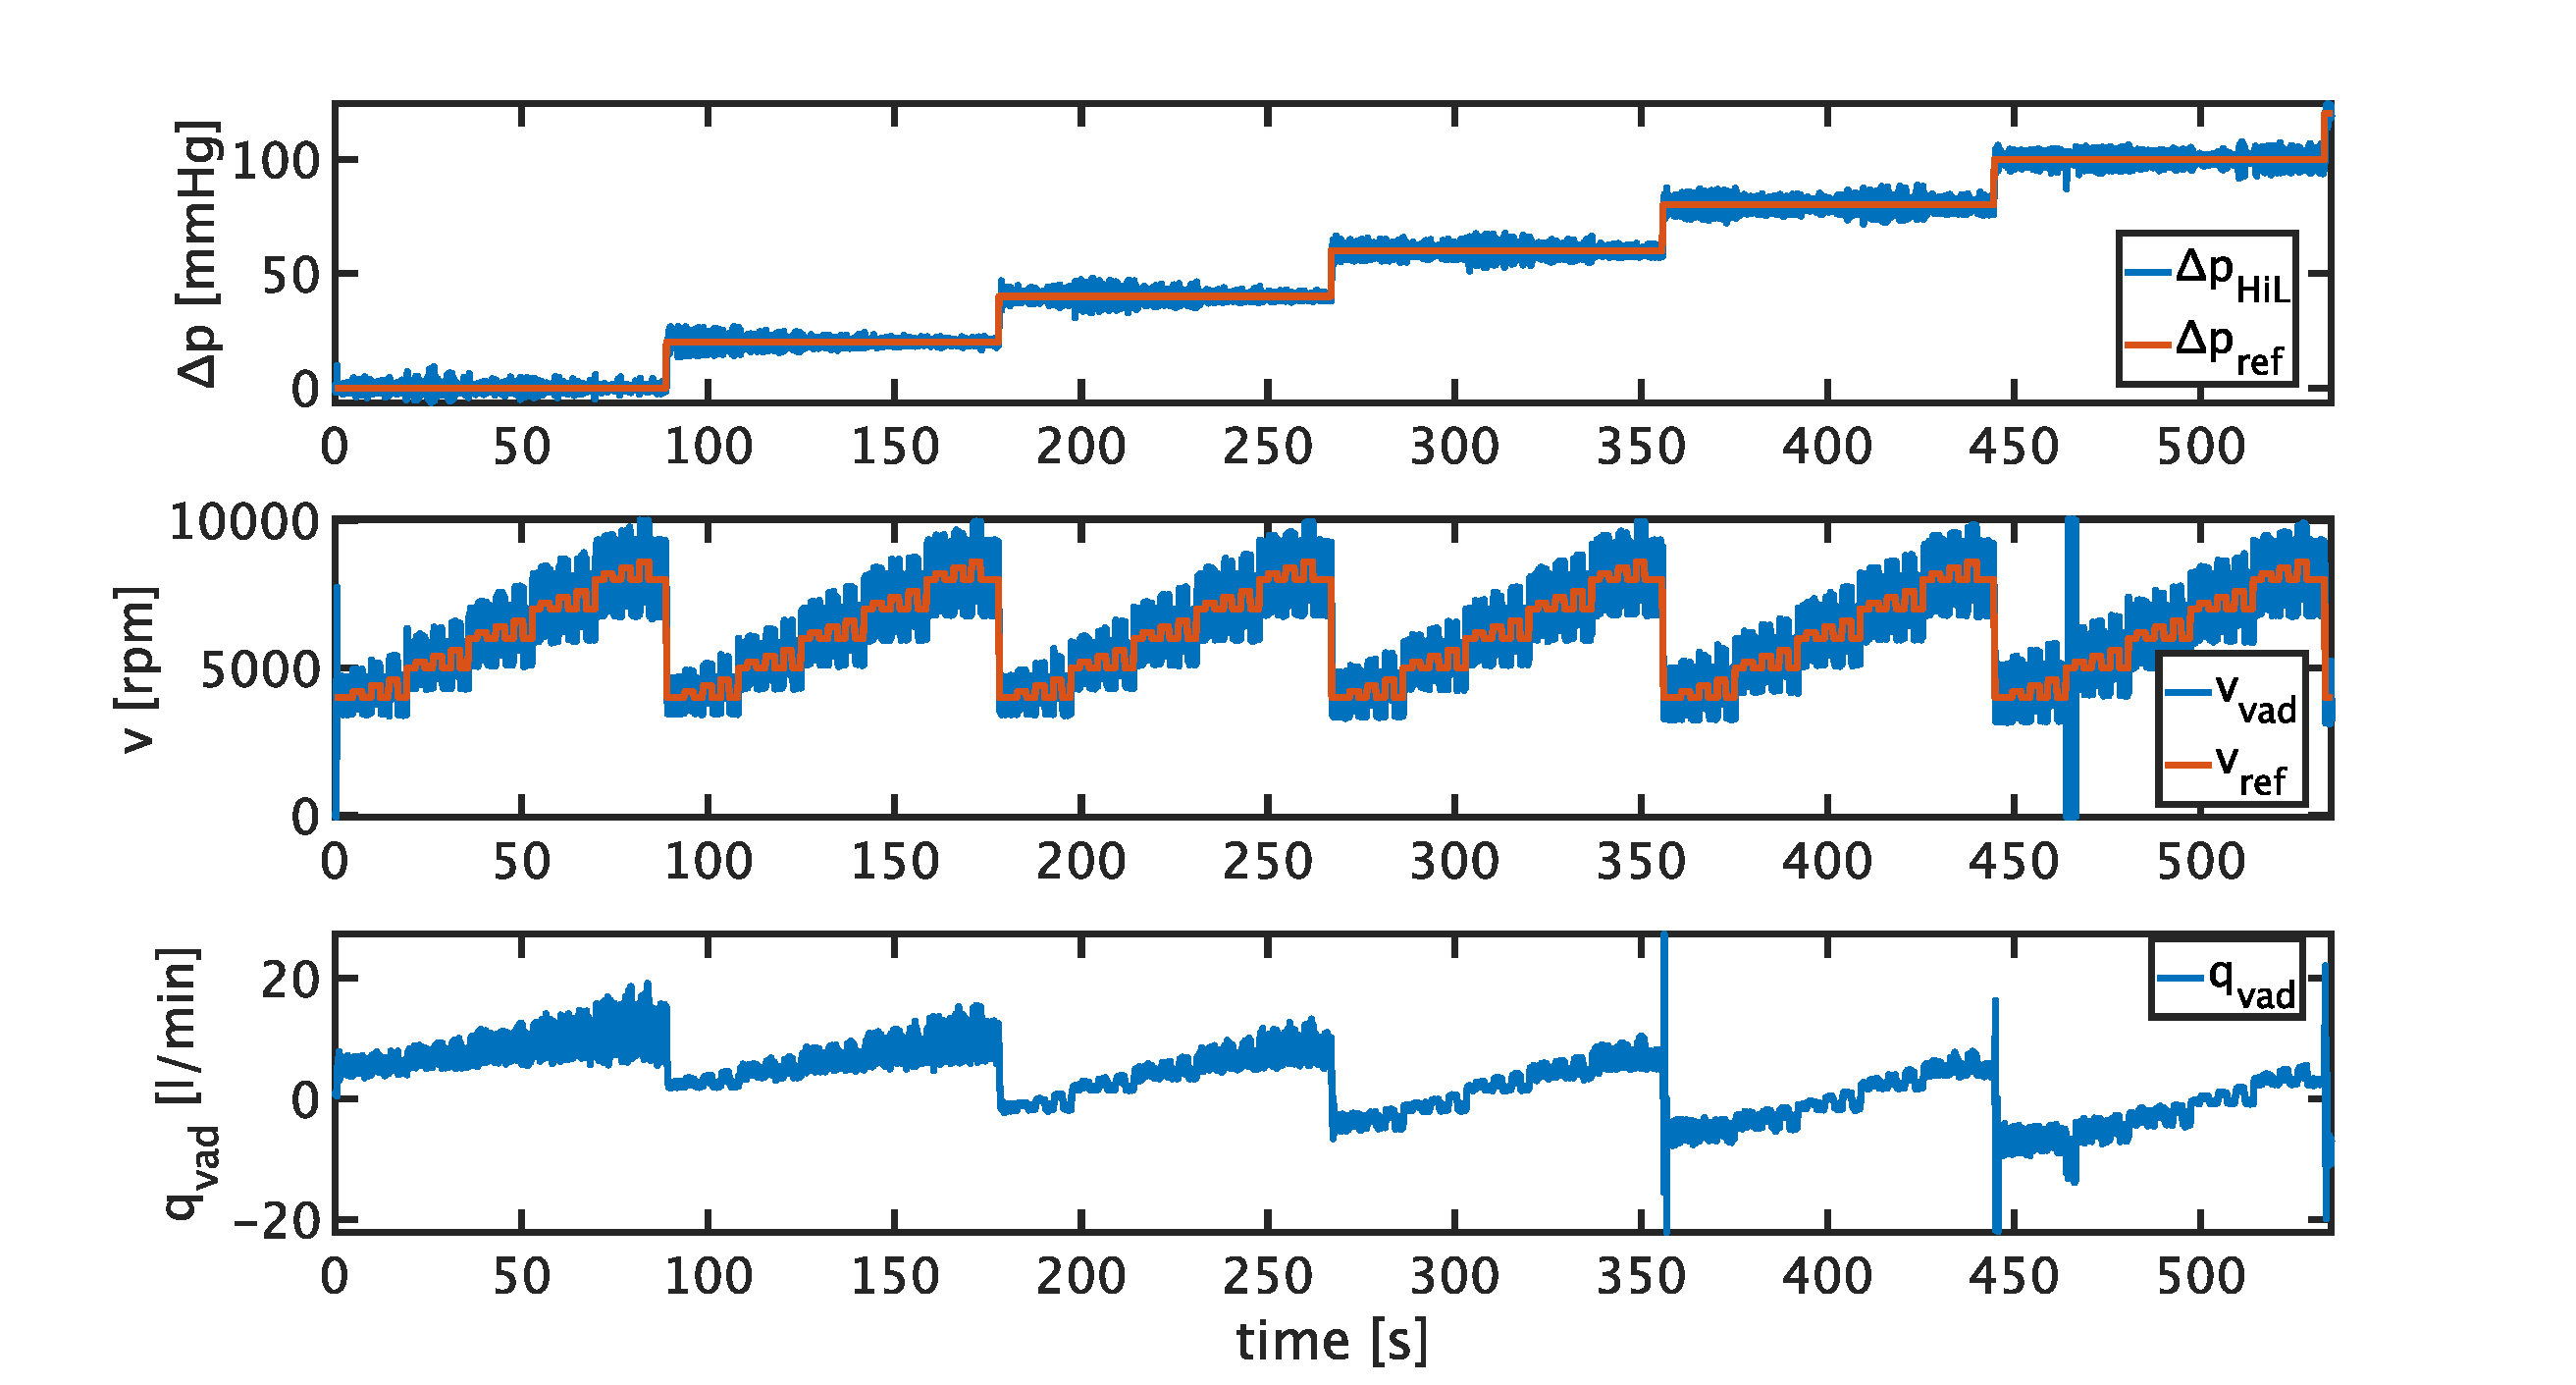
\includegraphics[width=0.95\textwidth]{images/chapt_5/dyn_measure.pdf}
  \caption[Signal curves for determination of PI controller parameters]{Signal curves for determination of PI controller parameters. Top: differential pressure as reference and measured signal, middle: reference and measured rotational speed, bottom: measured flow through Sputnik VAD.}
  \label{fig:dyn_meas}
\end{figure}
As presented in the upper graph, differential pressure is increased in steps of $20\,mmHg$ from $\Delta{p}=0\,mmHg$ to $\Delta{p}=100\,mmHg$. For each level the sequence of reference velocities depicted exemplary for $\Delta{p}=40\,mmHg$ in the center graph of \figurename~\ref{fig:dyn_meas_40} is targeted. Starting at $v_{\mathrm{ref}}=4000 \, rpm $ the velocity is first increased in three steps of varying height and then decreased by the same values. The first step amounts to $200 \, rpm$, the second to $400 \, rpm$ and the third to $600 \, rpm$. The reference value is then increased by $1000\,rpm$ and again the three steps are executed.
This sequential behavior is repeated up to a start value of $v_{\mathrm{ref}}=8000\,rpm$.
\begin{figure}[ht]
  \centering
  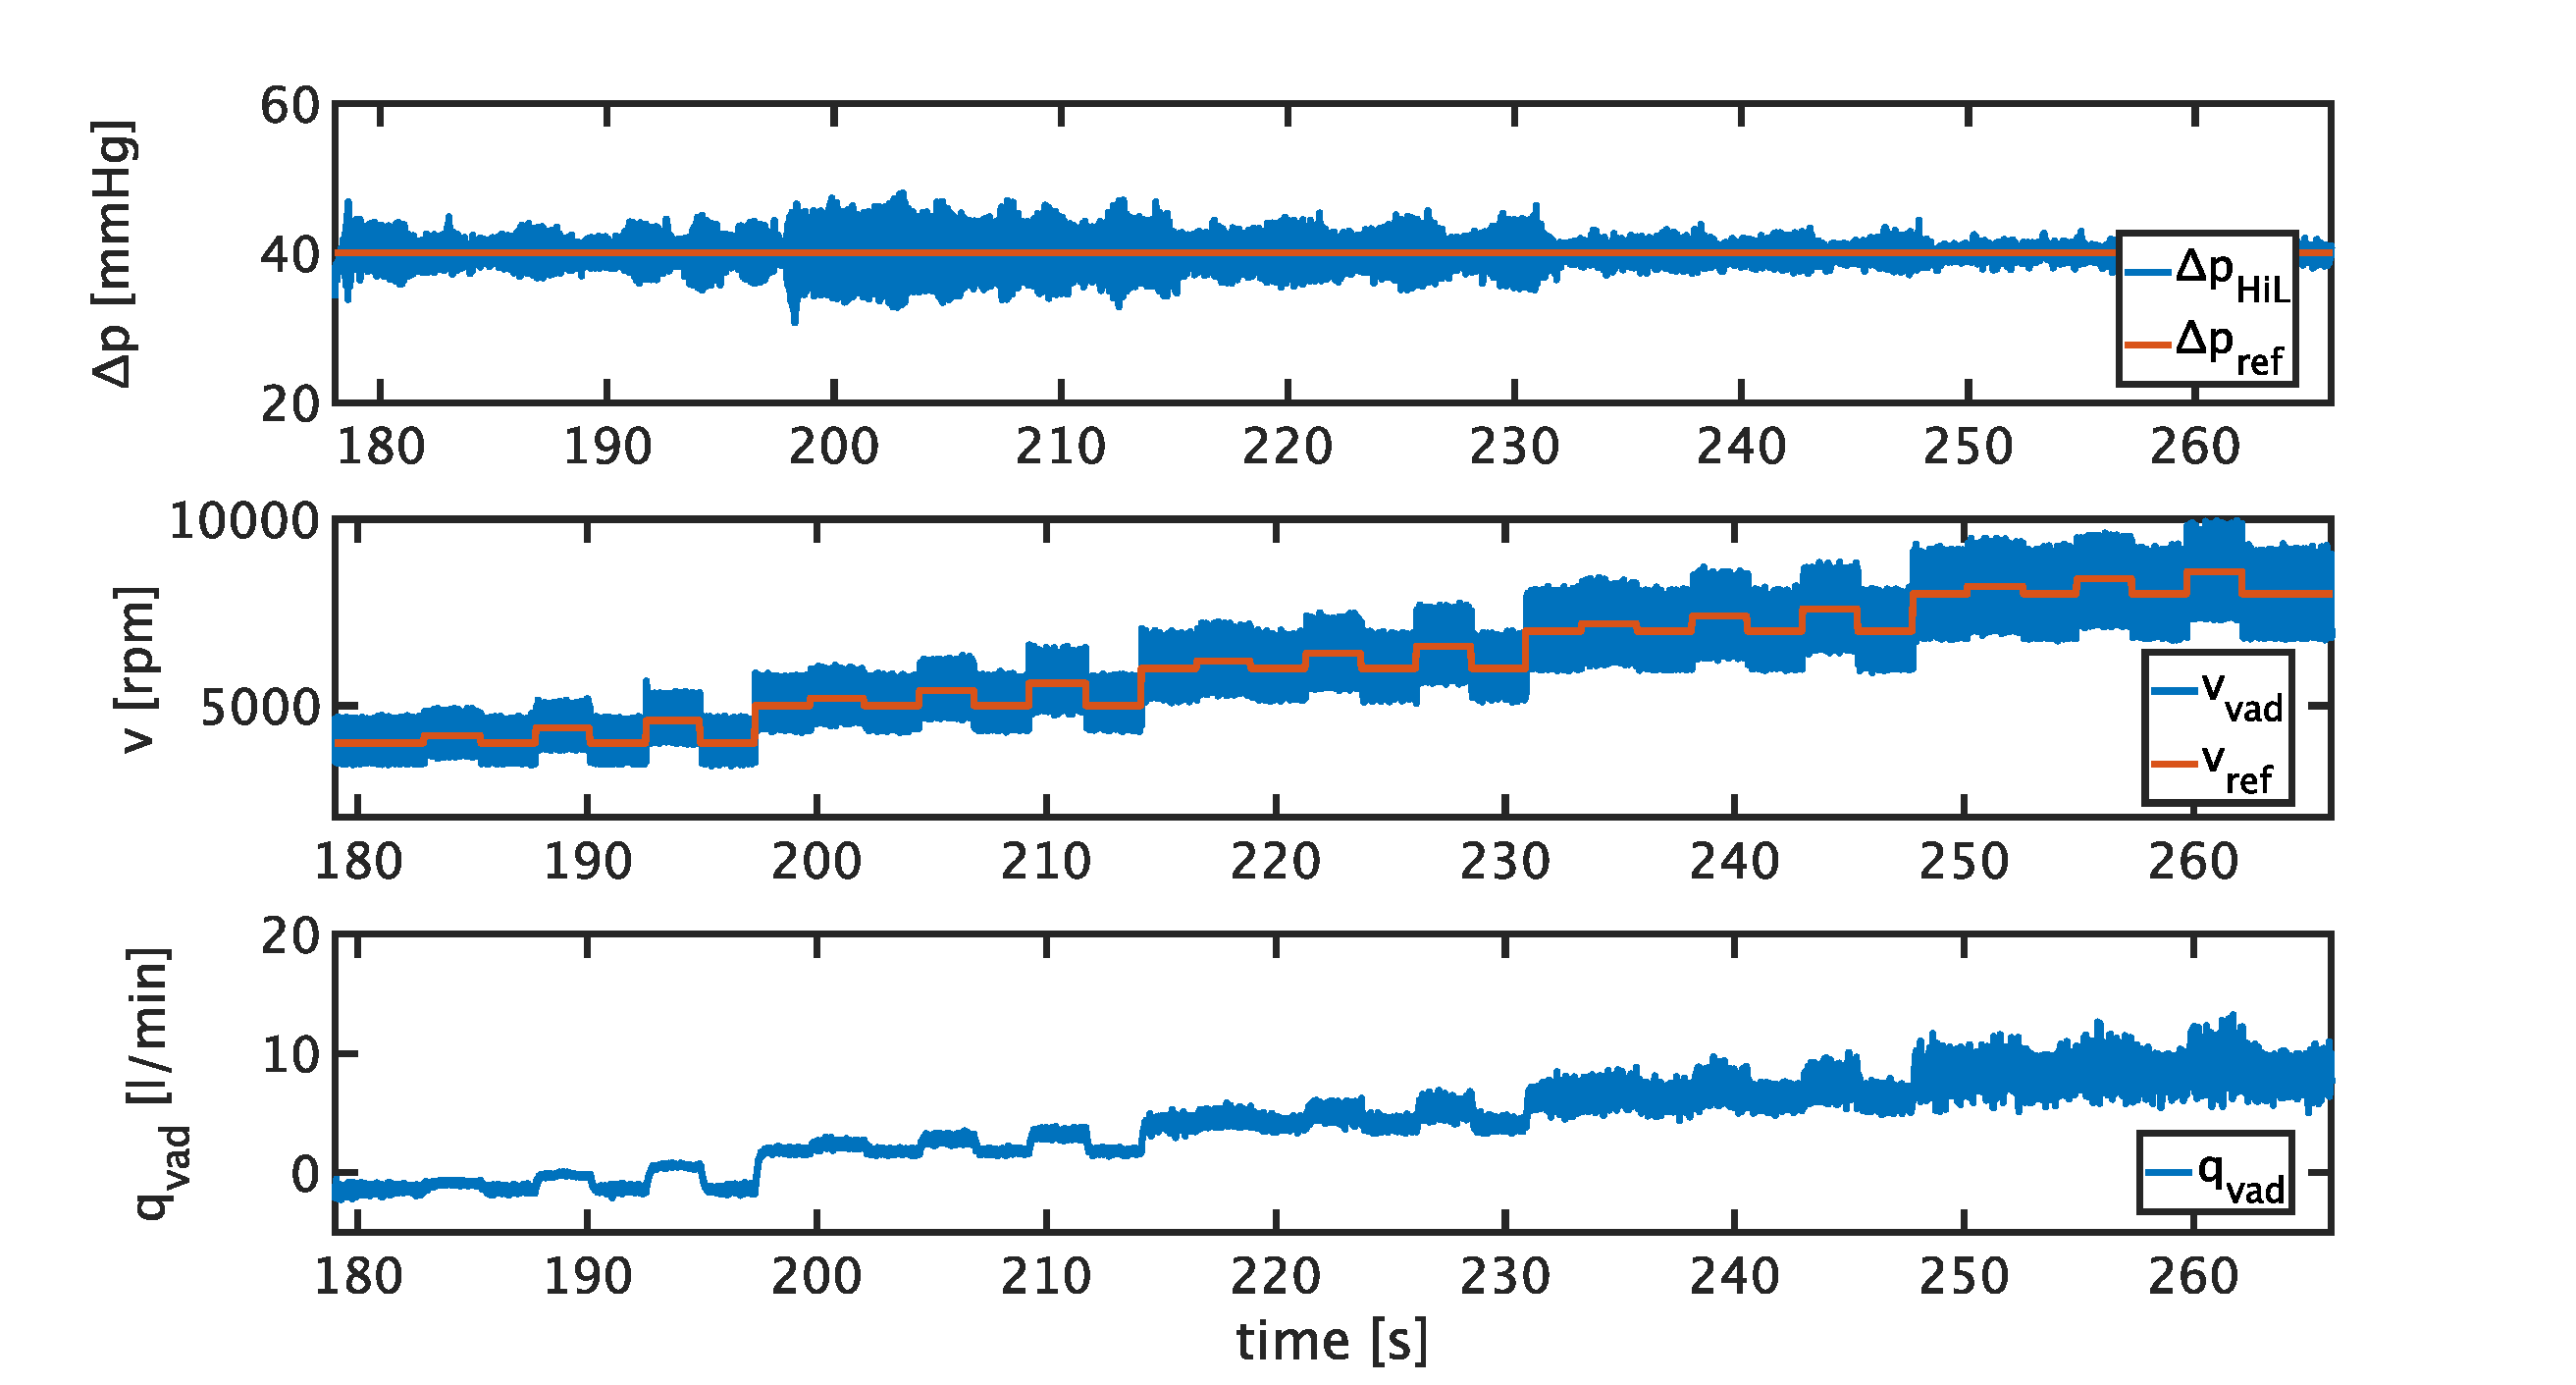
\includegraphics[width=\textwidth]{images/chapt_5/dyn_meas_40.pdf}
  \caption[Signal curves for determination of PI controller parameters at $\Delta{p}=40\,mmHg$]{Signal curves for determination of PI controller parameters at $\Delta{p}=40\,mmHg$.}
  \label{fig:dyn_meas_40}
\end{figure}
For determination of the parameters for controller design the step from $v_{\mathrm{ref,low}}=5000\, rpm$ to $v_{\mathrm{ref,high}}=5400\, rpm$ at $\Delta{p}=40\,mmHg$, which is located in the center of the pump's operating range, is used.
Since the flow signal is affected by high measurement noise, the signal is preprocessed using an $8^{th}$-order butterworth filter with cut off frequency $f_{\mathrm{c}}=5\,Hz$ and sampling frequency $f_{\mathrm{s}}=1000\,Hz$.
\begin{figure}[ht]
  \centering
  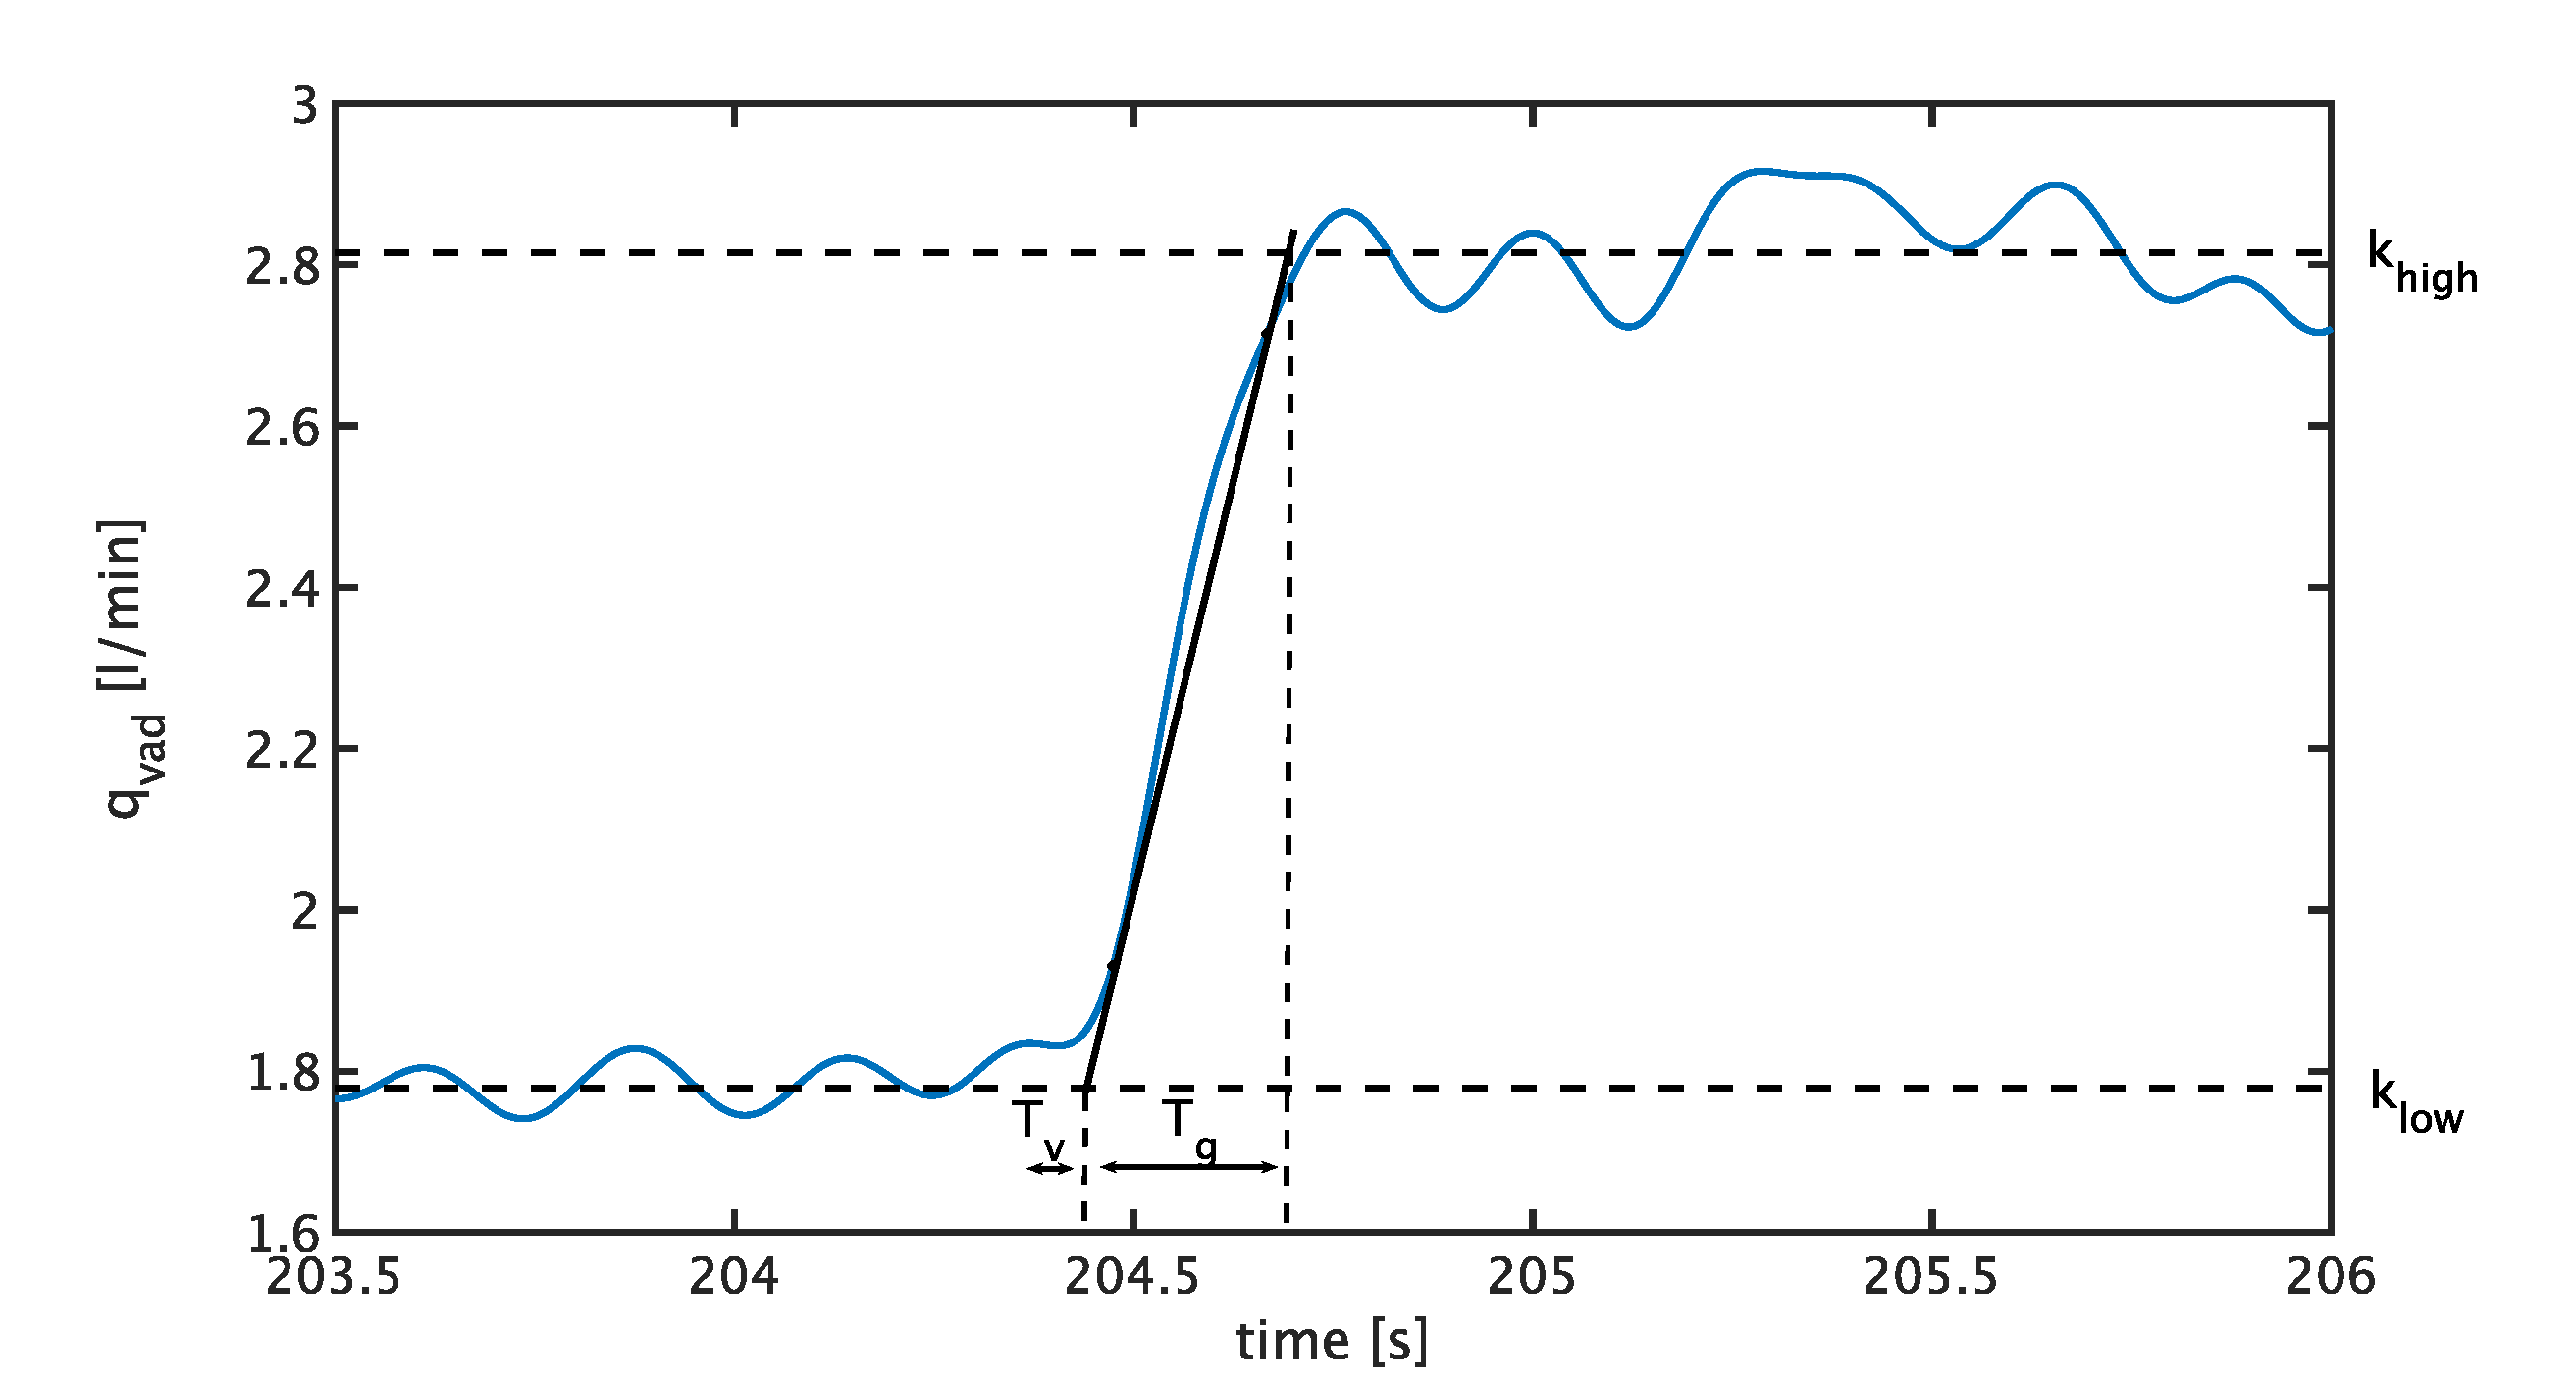
\includegraphics[width=0.95\textwidth]{images/chapt_5/param_calc_PI.pdf}
  \caption[Step response for determination of PI controller tuning parameters]{Step response for a step in rotational speed of $400\,rpm$ for determination of PI controller tuning parameters.}
  \label{fig:param_calc_PI}
\end{figure}
The resulting signal and the characteristic parameters needed for parameter tuning of the PI controller are depicted in \figurename~\ref{fig:param_calc_PI}. With $k_{\mathrm{high}}=2.8149$ and $k_{\mathrm{low}}=1.7783$ the static gain is determined as in equation (\ref{eq:k_s_1}) to
\begin{equation}
  k_{\mathrm{s}} = \frac{k_{\mathrm{high}}-k_{\mathrm{low}}}{v_{\mathrm{ref,high}}-v_{\mathrm{ref,low}}}= 0.0026.
\label{eq:k_s_2}
\end{equation}
The time constants amount to $T_{\mathrm{g}}=0.193$ and $T_{\mathrm{v}}=0.1$.
\\For determination of a PI controller tuned according to Ziegler Nichols equations (\ref{eq:kp_zn}) to (\ref{eq:T_N_zn}) are used. By this $K_{\mathrm{P}}$ is determined as
\begin{equation}
  K_{\mathrm{P}} = 0.9\cdot\frac{0.193}{0.0026\cdot0.1}=670.3052
\end{equation}
and $K_{\mathrm{I}}$ as
\begin{equation}
  K_{\mathrm{I}}  = \frac{670.3052}{3.3\cdot0.1}=2031.2278.
\end{equation}
Substituting these values in equation (\ref{eq:pi_contr_2}) results in the transfer function
\begin{equation}
  G_{\mathrm{PI,ZN}}(s)=670.3052+\frac{2031.2278}{s}.
\end{equation}
\\Calculation for overdamped controller behavior was chosen for controller tuning using Chien Hrones Reswick. Determination of the parameters $K_{\mathrm{P}}$ and $K_{\mathrm{I}}$ is performed following the equations presented in \tablename~\ref{tab:param_chr}, resulting in
\begin{equation}
  K_{\mathrm{P}} = 0.35\cdot\frac{0.193}{0.0026\cdot0.1}=260.6742
\end{equation}
and
\begin{equation}
  K_{\mathrm{I}} = \frac{260.6742}{1.2\cdot0.1}=2172.2853.
\end{equation}
This in turn leads to the transfer function
\begin{equation}
  G_{\mathrm{PI,CHR}}(s)=260.6742+\frac{2172.2853}{s}.
\end{equation}
\subsection{Evaluation}
The main purpose for utilization of a PI controller, in this work, is to stabilize the closed loop system behavior in preparation for an ILC implementation.
Both controllers are tested under the same operating conditions and their performance is compared.
\\Even though the controllers are tuned at $\Delta{p}=40\,mmHg$, both of them  are tested in the differential pressure operating range from $\Delta{p}=0\,mmHg$ to $\Delta{p}=100\,mmHg$ to ensure sufficient performance in all use cases.
For each differential pressure level three consecutive steps up and down throughout the operating range of flow are performed. Each reference flow is targeted for $5\,s$ and flow through the VAD is measured. A graphical representation of the reference signal curves is depicted in \figurename~\ref{fig:PI_control_ref_signals}.
\begin{figure}[ht]
  \centering
  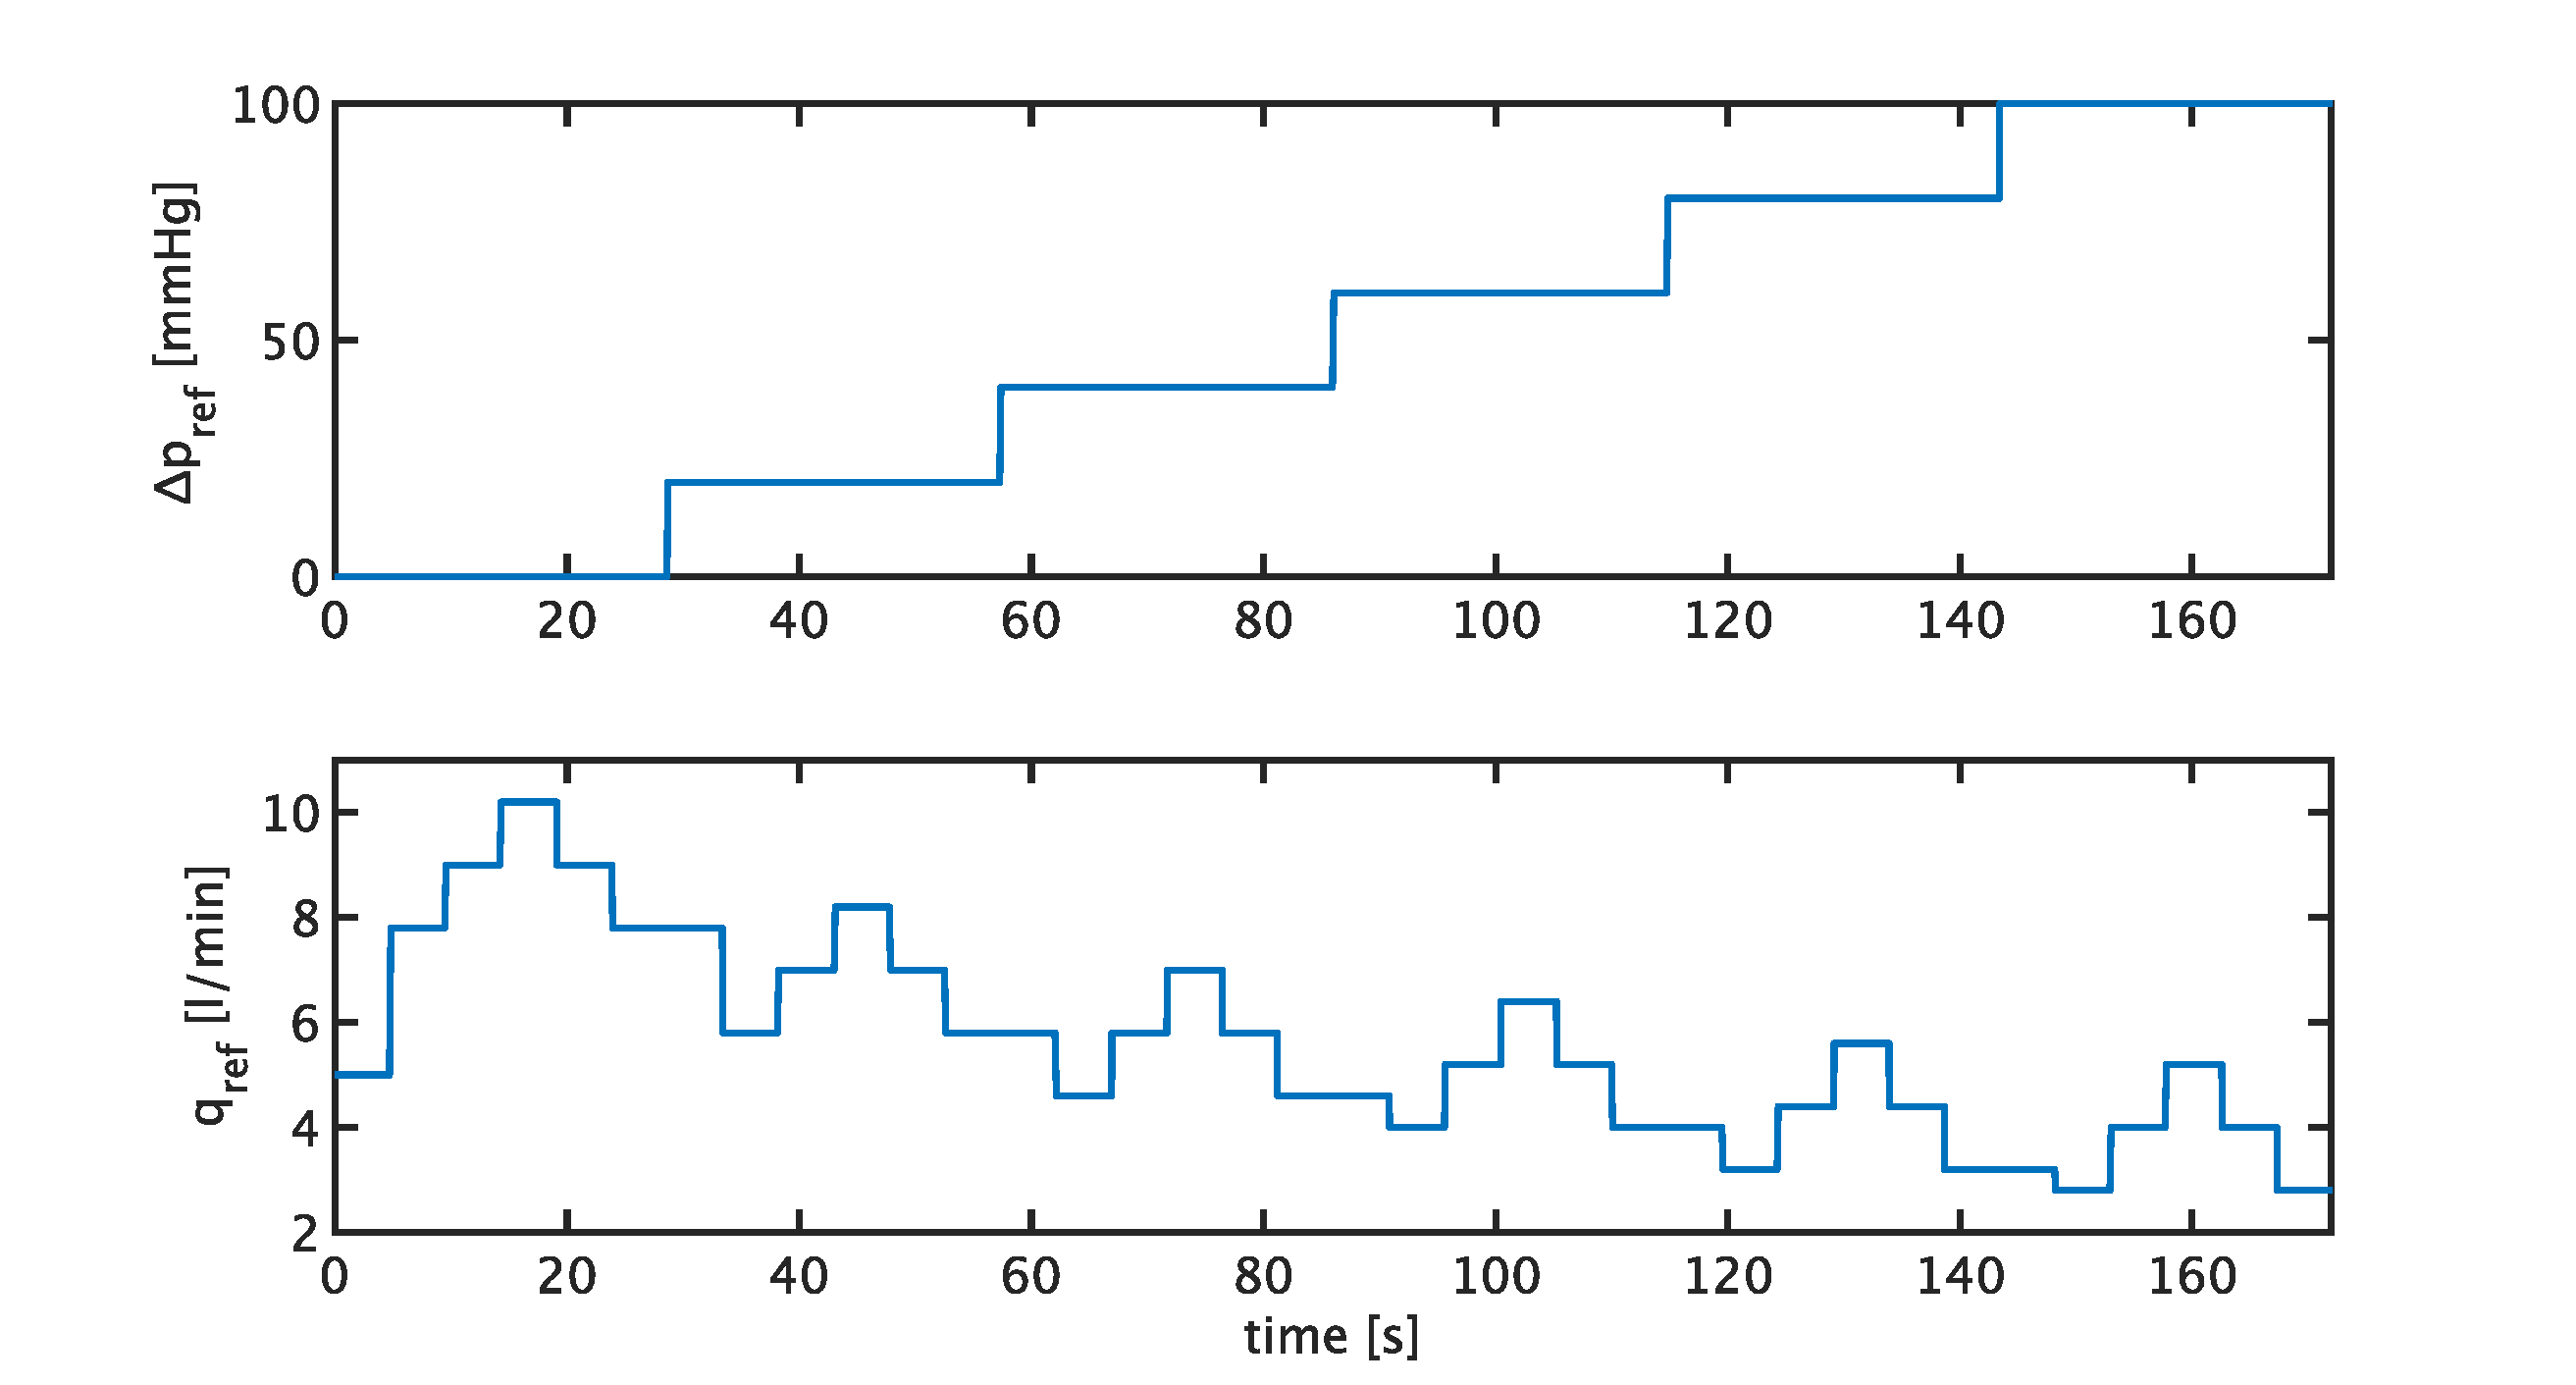
\includegraphics[width=0.95\textwidth]{images/chapt_5/PI_control_ref_signals.pdf}
  \caption[Reference signals for PI controller performance evaluation]{Reference signals for PI controller performance evaluation. Top: differential pressure reference value. Bottom: targeted flow trajectory.}
  \label{fig:PI_control_ref_signals}
\end{figure}
\figurename~\ref{fig:pi_contr_chr_40} depicts the differential pressure and flow reference values, the measured pressure and flow value and the actuation variable in form of the reference rotational speed $v_{\mathrm{act}}$ and rotational speed of the VAD $v_{\mathrm{vad}}$ for the differential pressure level $\Delta{p}=40\,mmHg$ using the PI controller tuned according to Chien Hrones Reswick.
\begin{figure}[ht]
  \centering
  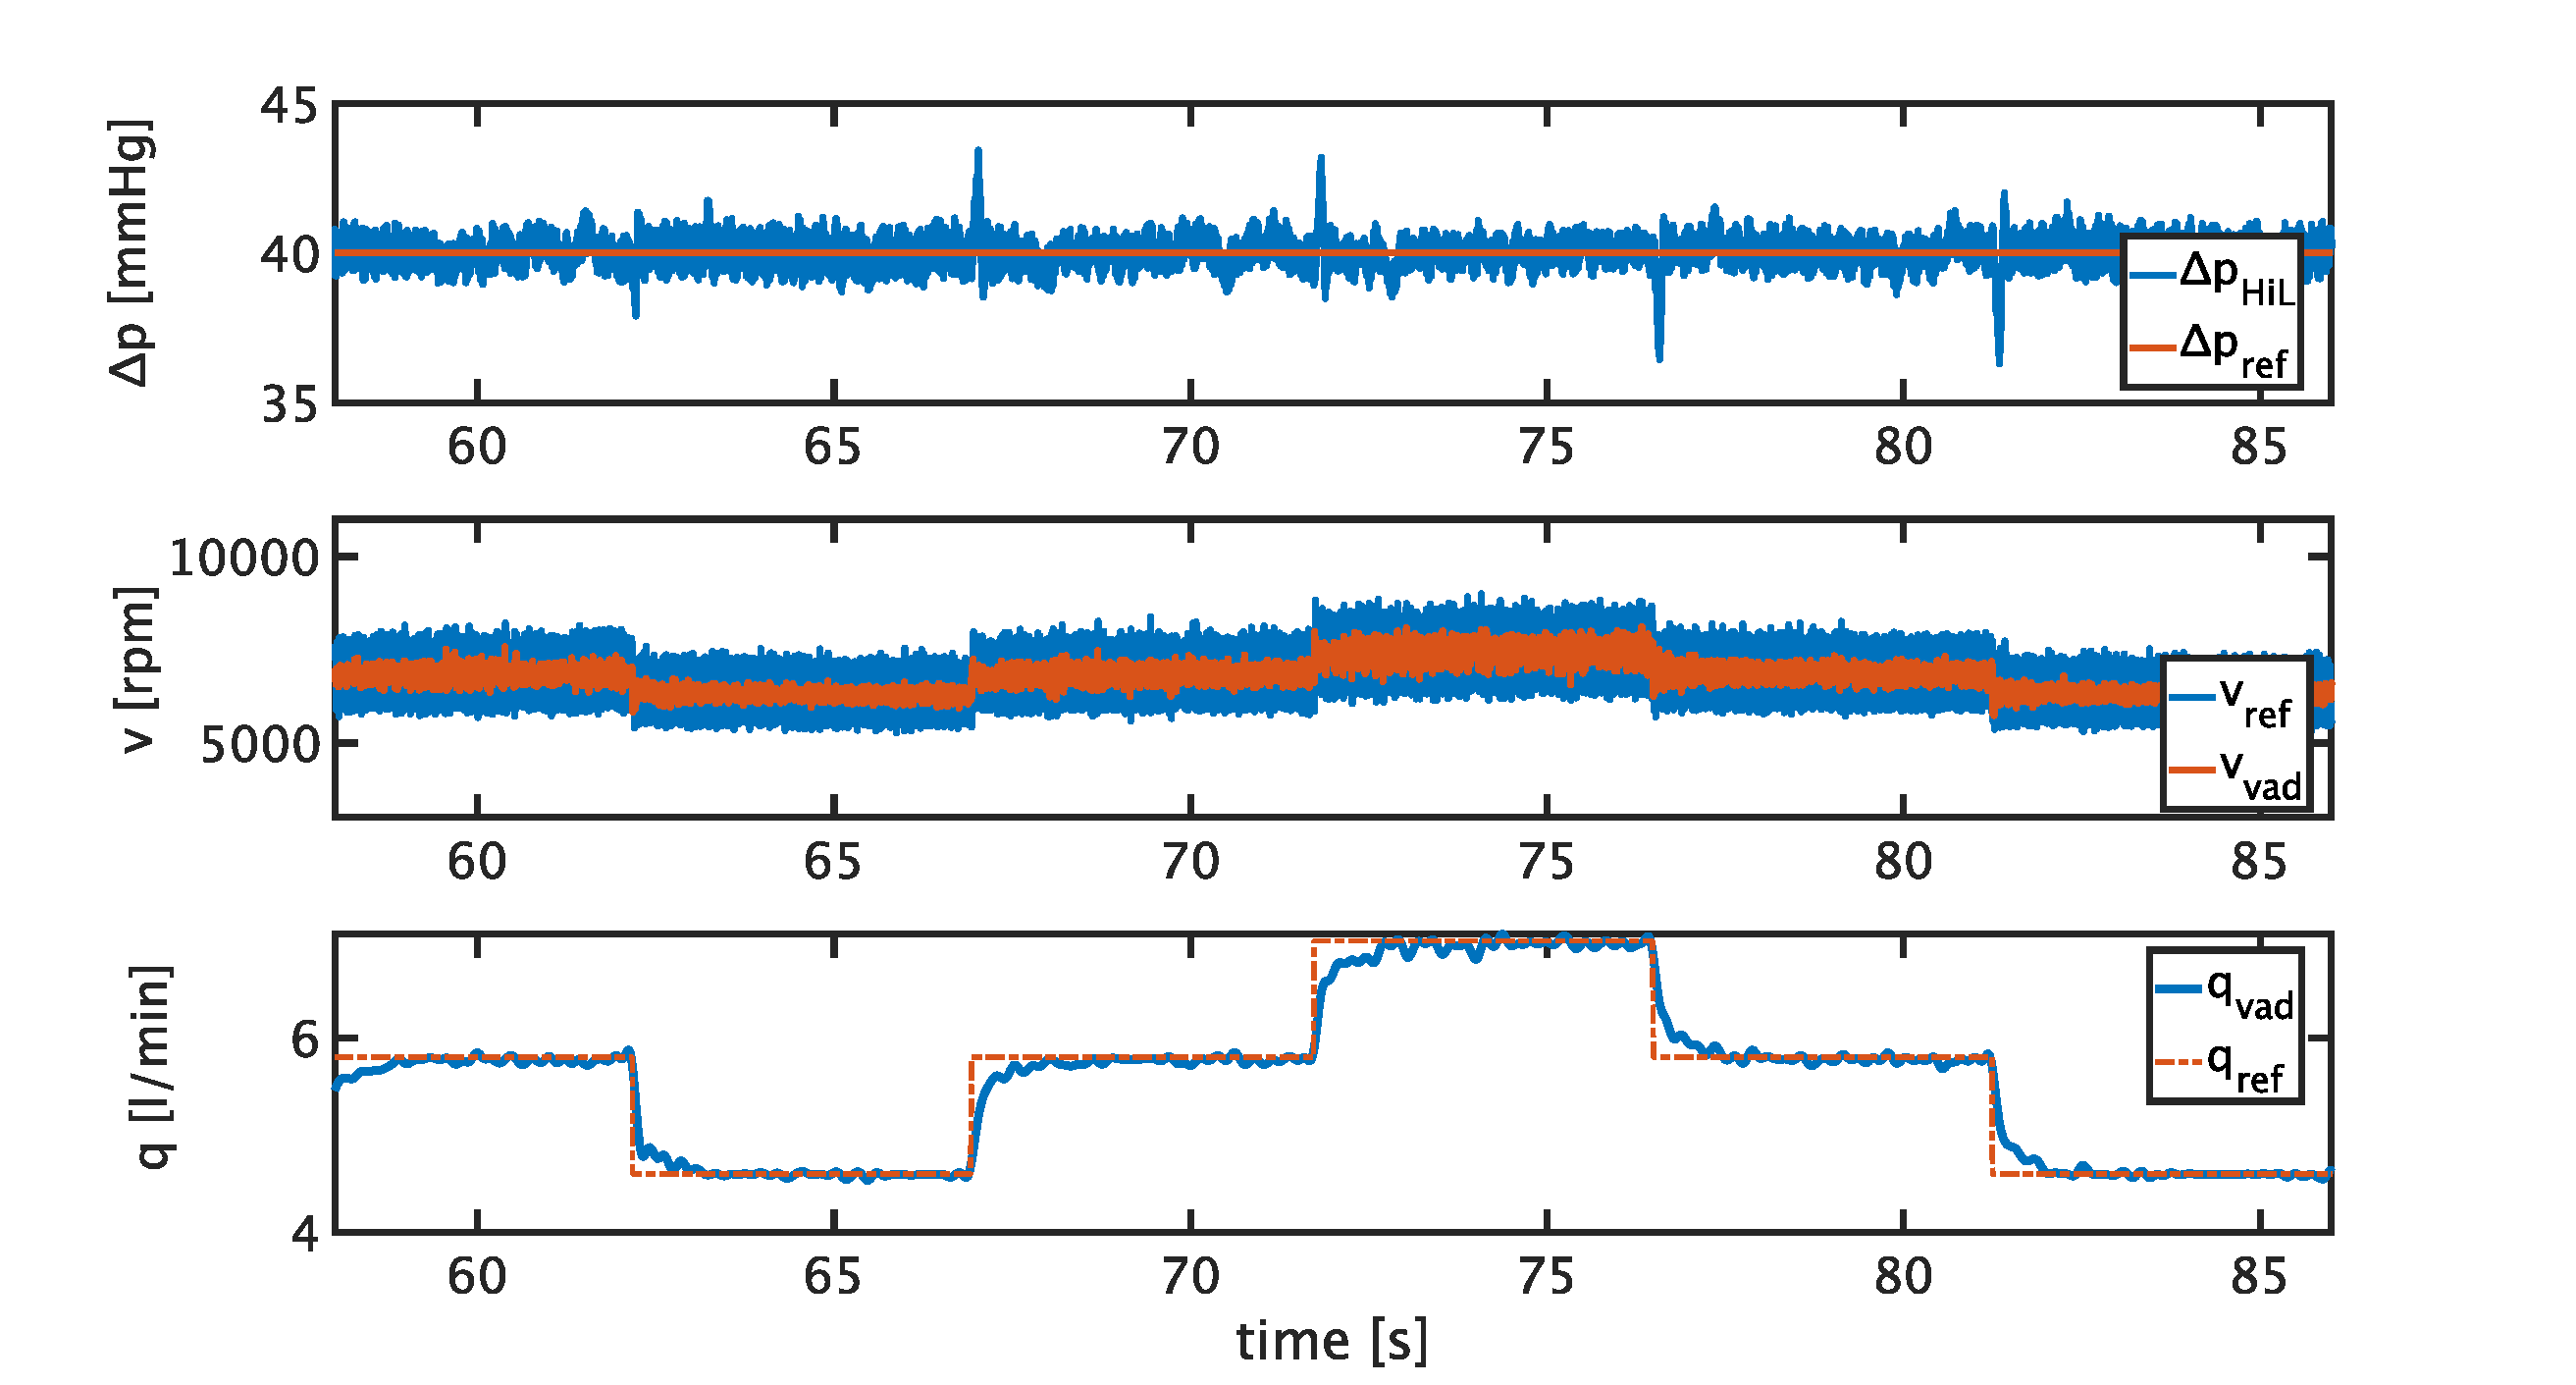
\includegraphics[width=0.9\textwidth]{images/chapt_5/pi_contr_chr_40.pdf}
  \caption[Test measurement for PI controller tuned according to Chien Hrones Reswick at $\Delta{p}=40\,mmHg$]{Test measurement for PI controller tuned according to Chien Hrones Reswick at $\Delta{p}=40\,mmHg$.}
  \label{fig:pi_contr_chr_40}
\end{figure}
\\The complete signal curves for the tests of the controllers are depicted in \figurename~\ref{fig:anh_6} and \figurename~\ref{fig:anh_7} in the appendix. Furthermore, the graphical representation of the test measurement at $\Delta{p}=40\,mmHg$ for the controller tuned according to Ziegler Nichols is depicted in \figurename~\ref{fig:anh_8} of the appendix.
\\The course of the control error throughout the test measurements of the controller tuned according to Ziegler Nichols and the controller tuned according to Chien Hrones Reswick are depicted in \figurename~\ref{fig:PI_error_a} and \figurename~\ref{fig:PI_error_b}, respectively.
\begin{figure}[ht]
  \centering
  \subfloat[]
  {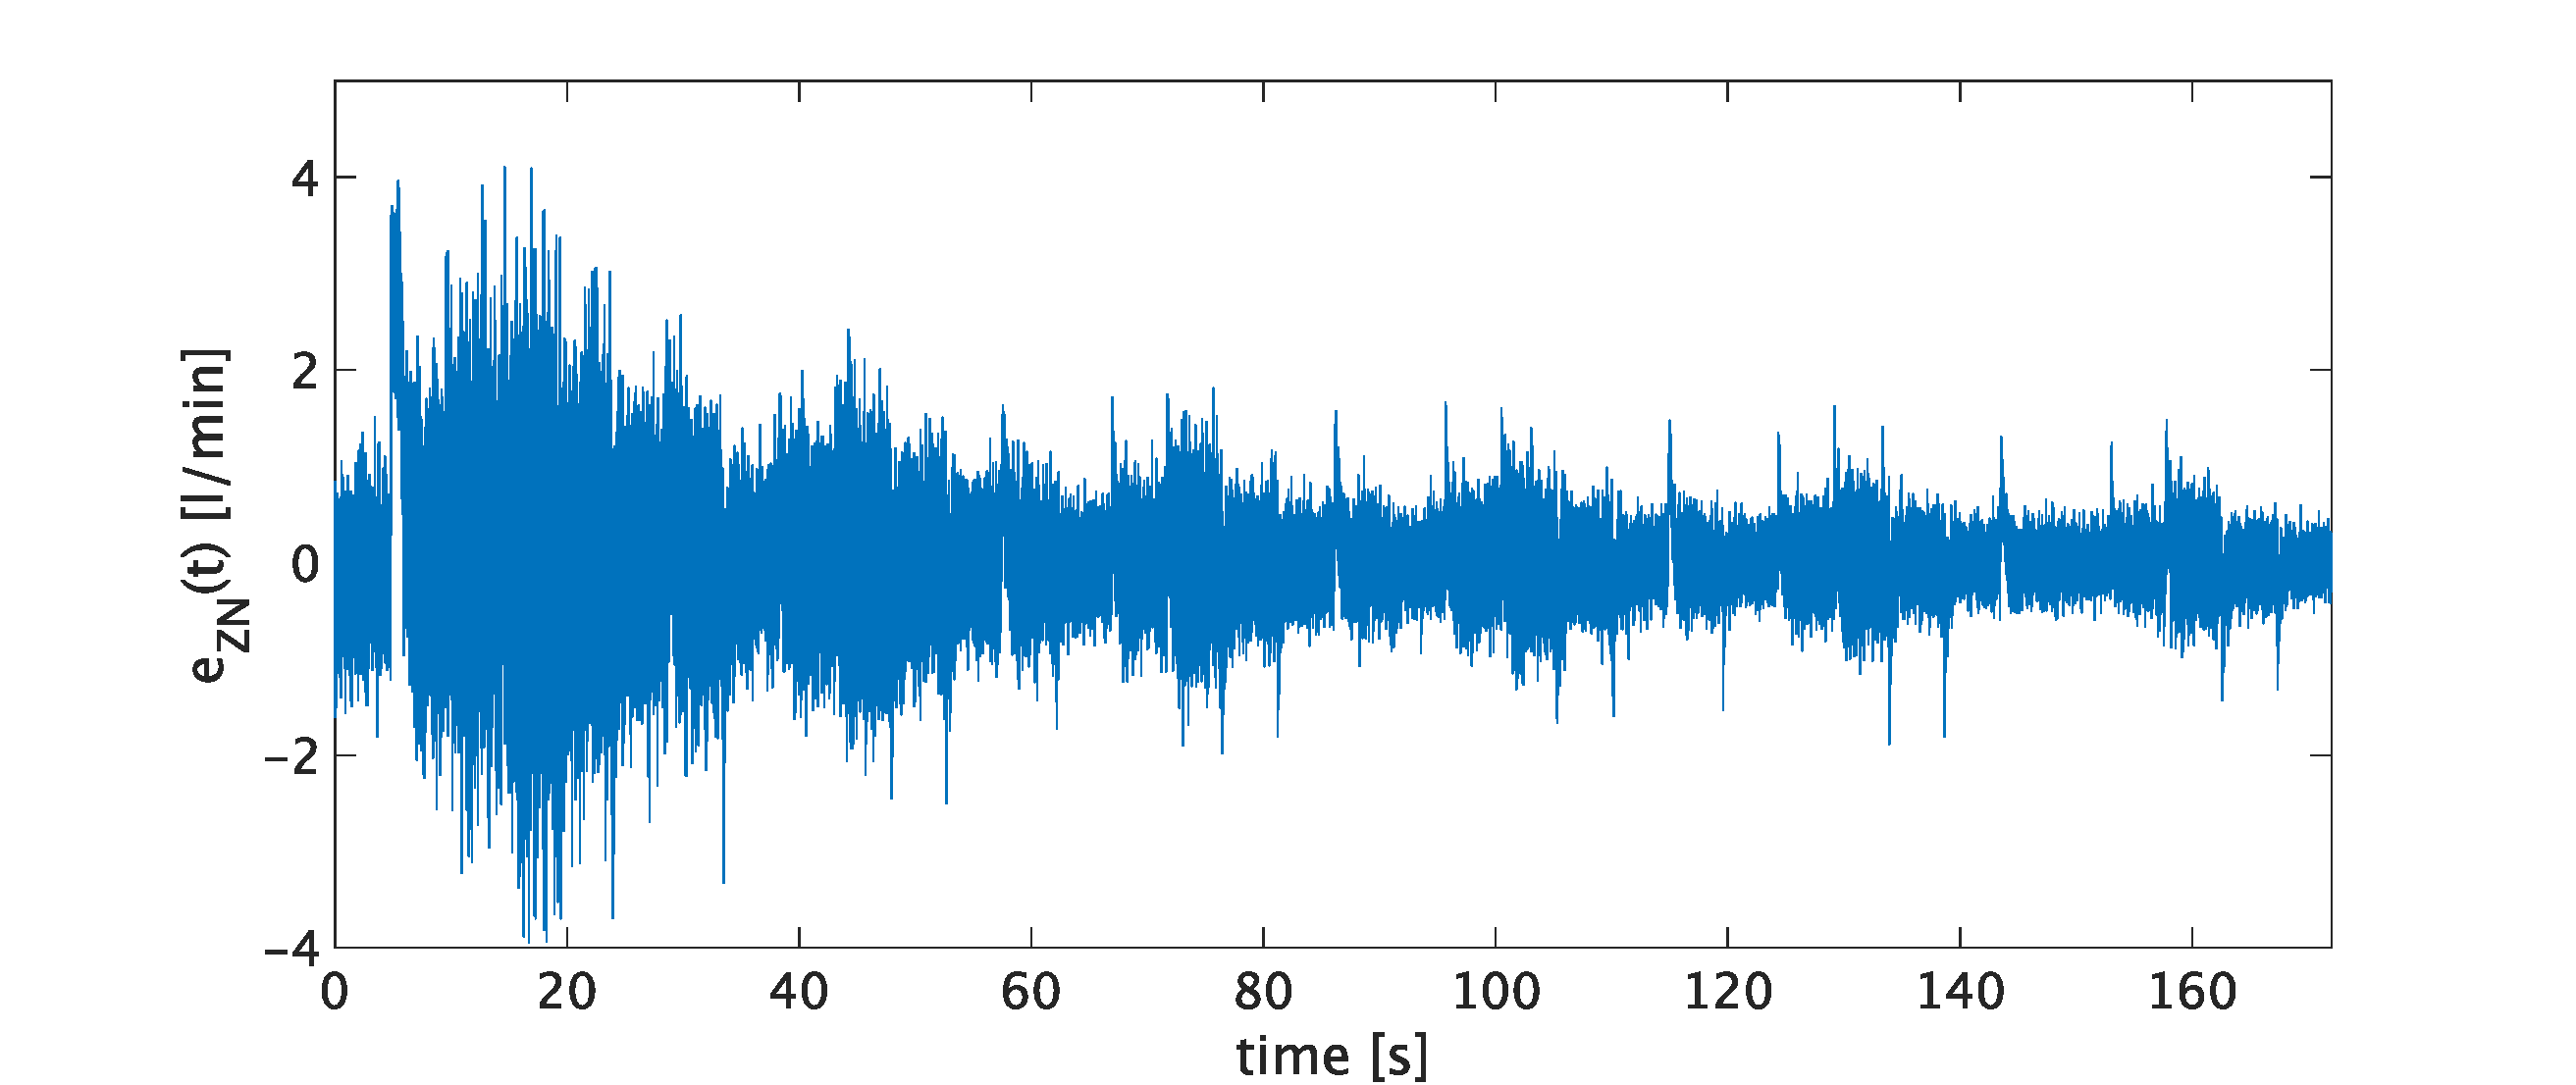
\includegraphics[width=0.5\textwidth]{images/chapt_5/error_PI_zn.pdf}\label{fig:PI_error_a}}
  \subfloat[]
  {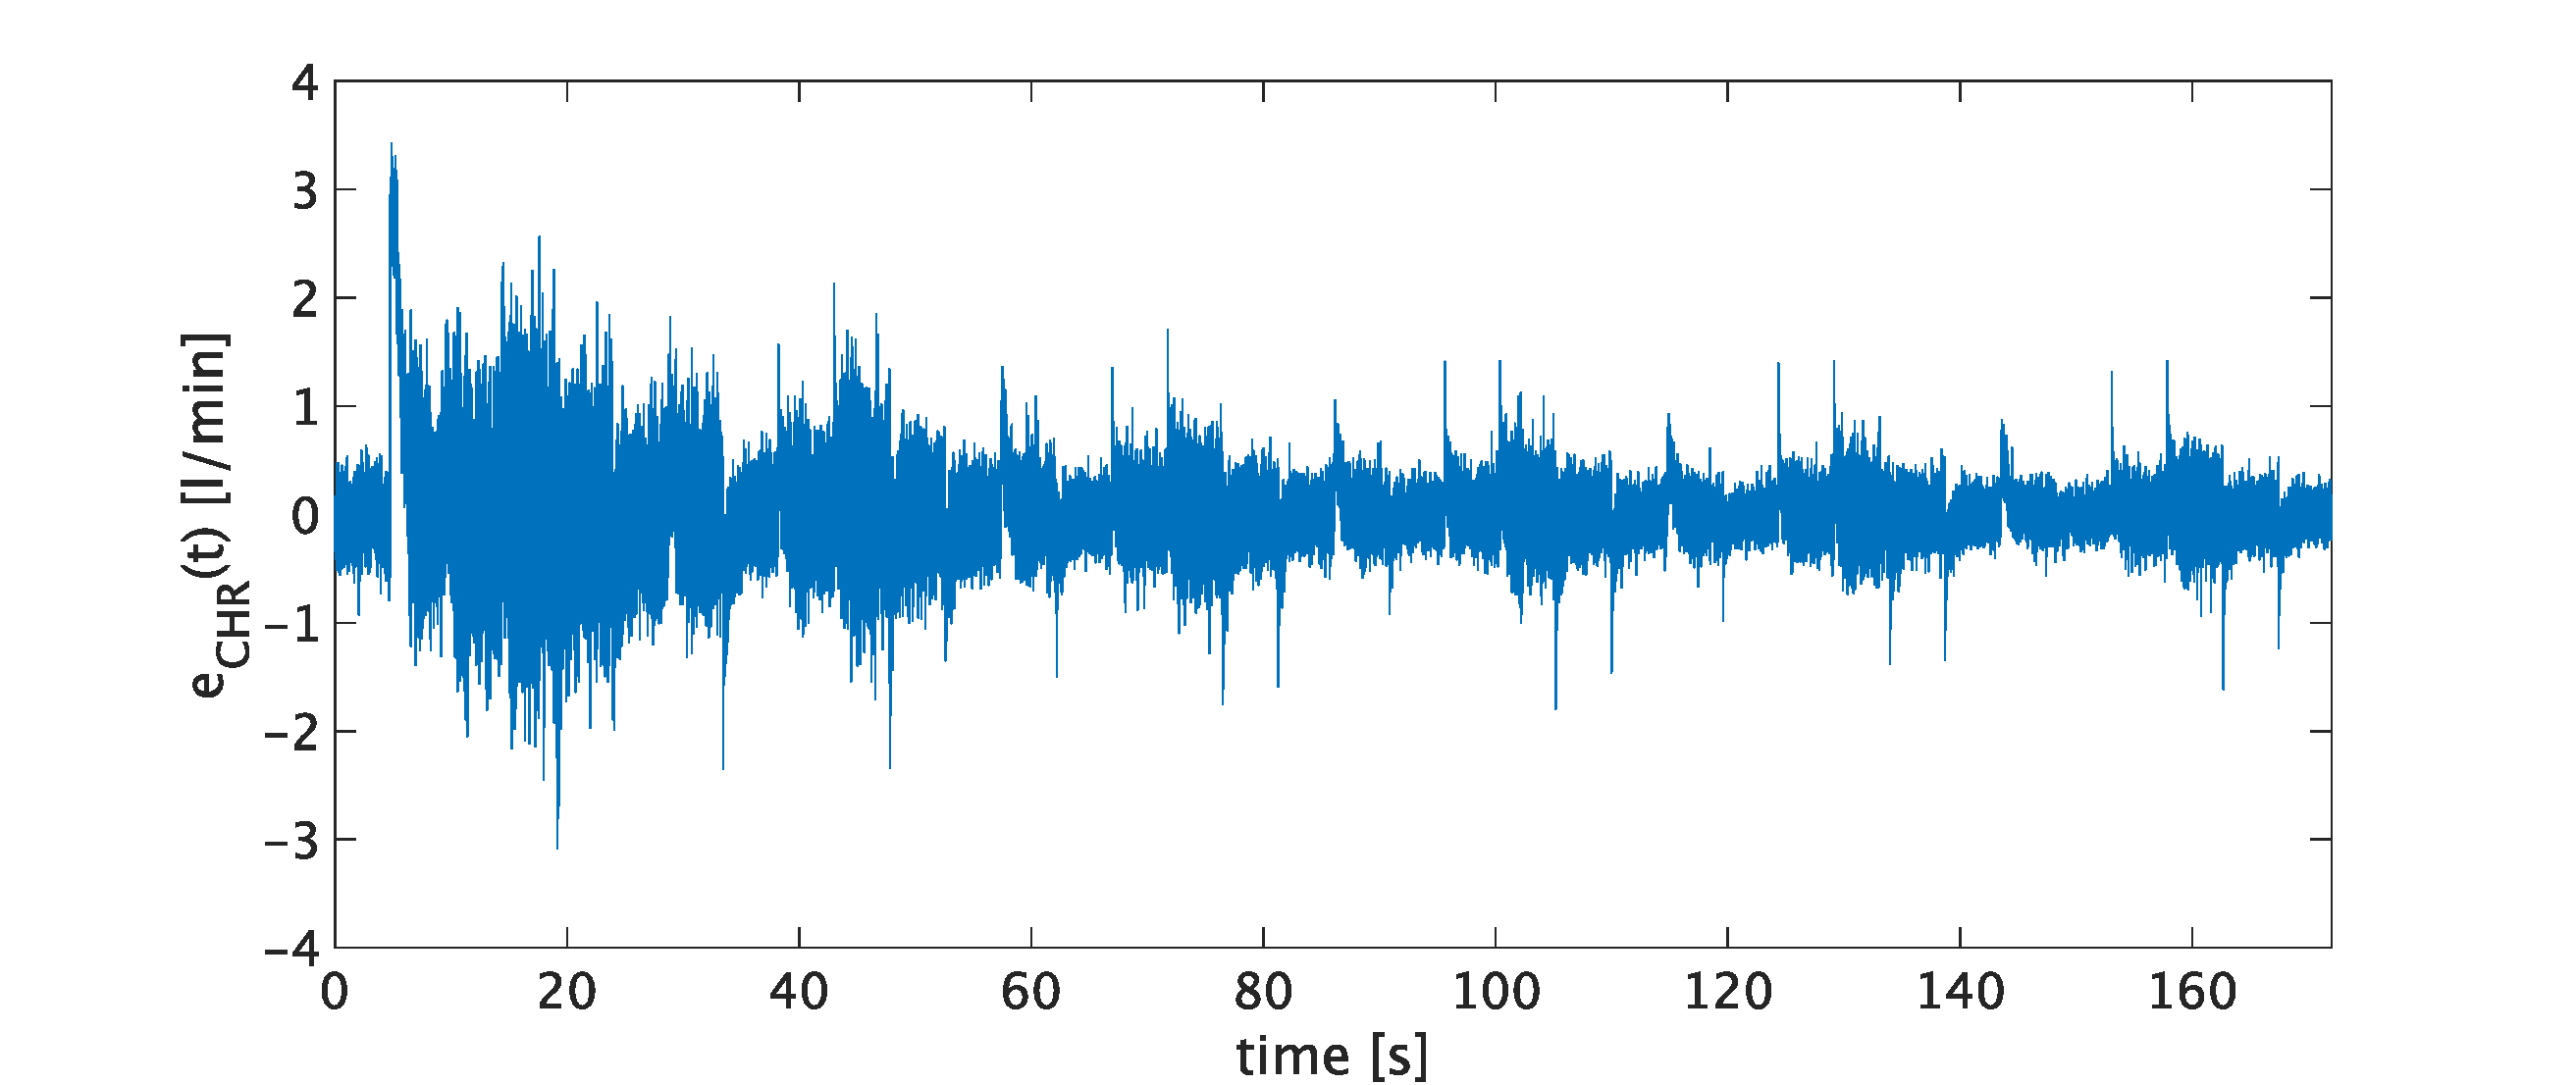
\includegraphics[width=0.5\textwidth]{images/chapt_5/error_PI_chr.pdf}\label{fig:PI_error_b}}
  \caption[Control error for PI Controllers]{Control error for PI controllers tuned according to (a) Ziegler Nichols, (b) Chien Hrones Reswick}
  \label{fig:PI_error}
\end{figure}
\\Throughout this work, for evaluation of controller performance the root mean square error (RMSE), according to \cite{RMSE}, defined as
\begin{equation}
  RMSE = \sqrt{\frac{1}{n}\sum_{i=0}^n e_i^2}
\end{equation}
is used. The RMSE for the differential pressure level of $\Delta{p}=40\,mmHg$ for Ziegler Nichols tuned controller amounts to
\begin{equation}
  RMSE_{\mathrm{ZN,40}}=0.4013\,l/min
\end{equation}
while RMSE of the Chien Hrones Reswick tuned controller amounts to
\begin{equation}
  RMSE_{\mathrm{CHR,40}}=0.2753\,l/min.
\end{equation}
Taking into account the full differential pressure operating range for RMSE calculation these values amount to
\begin{equation}
  RMSE_{\mathrm{ZN}}=0.5396\,l/min
\end{equation}
and
\begin{equation}
  RMSE_{\mathrm{CHR}}=0.3705\,l/min.
\end{equation}
Comparing these results it is evident that both controllers perform more precise in the range of $\Delta{p}=40\,mmHg$, for which tuning has been performed.
Performance of the controller tuned according to Chien Hrones Reswick surpasses the Ziegler Nichols tuned one in both ranges. RMSE values for full range CHR control even indicate a higher performance in comparison to the Ziegler Nichols tuned controller in the range of $\Delta{p}=40\,mmHg$.
\\ Due to its higher performance, for all following measurements the PI controller tuned in reference to Chien Hrones Reswick is used.
\section{Iterative Learning Control}\label{ILC_1}
As shown in \figurename~\ref{fig:pi_contr_chr_40}, the exclusive use of a PI controller for flow control leads to necessity of long measurement times to allow the flow to settle at a new reference value. However, one goal of this thesis is to enable flow control following different reference trajectories which may imply the need for faster reference tracking. By implementing an ILC approach, the necessary reduction of settling time, by gaining information from error values of the preceding iteration, should be made possible.
\subsection{Design and Implementation}
During this work a P-type ILC is implemented and optimized.
\\The implementation is based on a parallel architecture as depicted in \figurename~\ref{fig:ILC_parallel}. This leads to the basic learning function for this ILC being represented by
\begin{equation}
  u_{\mathrm{j+1}}(k) = u_{\mathrm{j}}(k)+k_{\mathrm{p}}e_{\mathrm{j}}(k).
\end{equation}
The learning gain $k_{\mathrm{p}}$ is experimentally chosen as
\begin{equation}
  k_{\mathrm{p}} = 225
\end{equation}
to ensure quick error convergence.
\\As described in chapter \ref{ILC}, the basic ILC is extended to include a Q-Filter to enable more precise tuning of the ILC and increase its robustness.
This expansion results in the learning function being described by
\begin{equation}
  u_{\mathrm{j+1}}(k) = Q(q)[u_{\mathrm{j}}(k)+k_{\mathrm{p}}e_{\mathrm{j}}(k)].
\end{equation}
The Q-Filter is implemented as a $2^{nd}$-order butterworth filter, with sampling frequency $f_{\mathrm{s}}=1000\,Hz$. The cut off frequency $f_{\mathrm{c}}$ is set to several values in order to compare and thus optimize performance and robustness of the iterative learning control system.
\\An additional part of the implementation is the generation of a repeating reference and a trigger signal. The trigger signal indicates the beginning of each new iteration and thus initiates calculation of the new values $u_{\mathrm{j+1}}(k)$ in the ILC block.
\figurename~\ref{fig:ref_signal_ILC3} depicts three iterations of the reference signal for this ILC.
\\The signal is created by first generating a square wave signal with the upper stage at $6\, l/min$ and the lower stage at $4\, l/min$. Thus, the signal encloses the average value of $5\, l/min$ of the cardiac output of a healthy heart. The reference values are each held for $0.5\, s$, so that a complete iteration would correspond to a frequency of $60\, beats\, per\, minute\, (bpm)$ when compared to the heart rate. To avoid abrupt transitions in flow, which could lead to problems on the part of the pump, the reference signal was filtered with a first order Butterworth filter with cut off frequency $f_{\mathrm{c}}=20\,Hz$ and sampling frequency $f_{\mathrm{s}}=1000\,Hz$, resulting in radiused transitions. Afterwards, the signal is shifted by $0.25\, s$ to avoid placing the beginning of the signal at a jump point. The trigger signal is set from 0 to 1 at the beginning of each iteration for the duration of one sample.
\begin{figure}[ht]
  \centering
  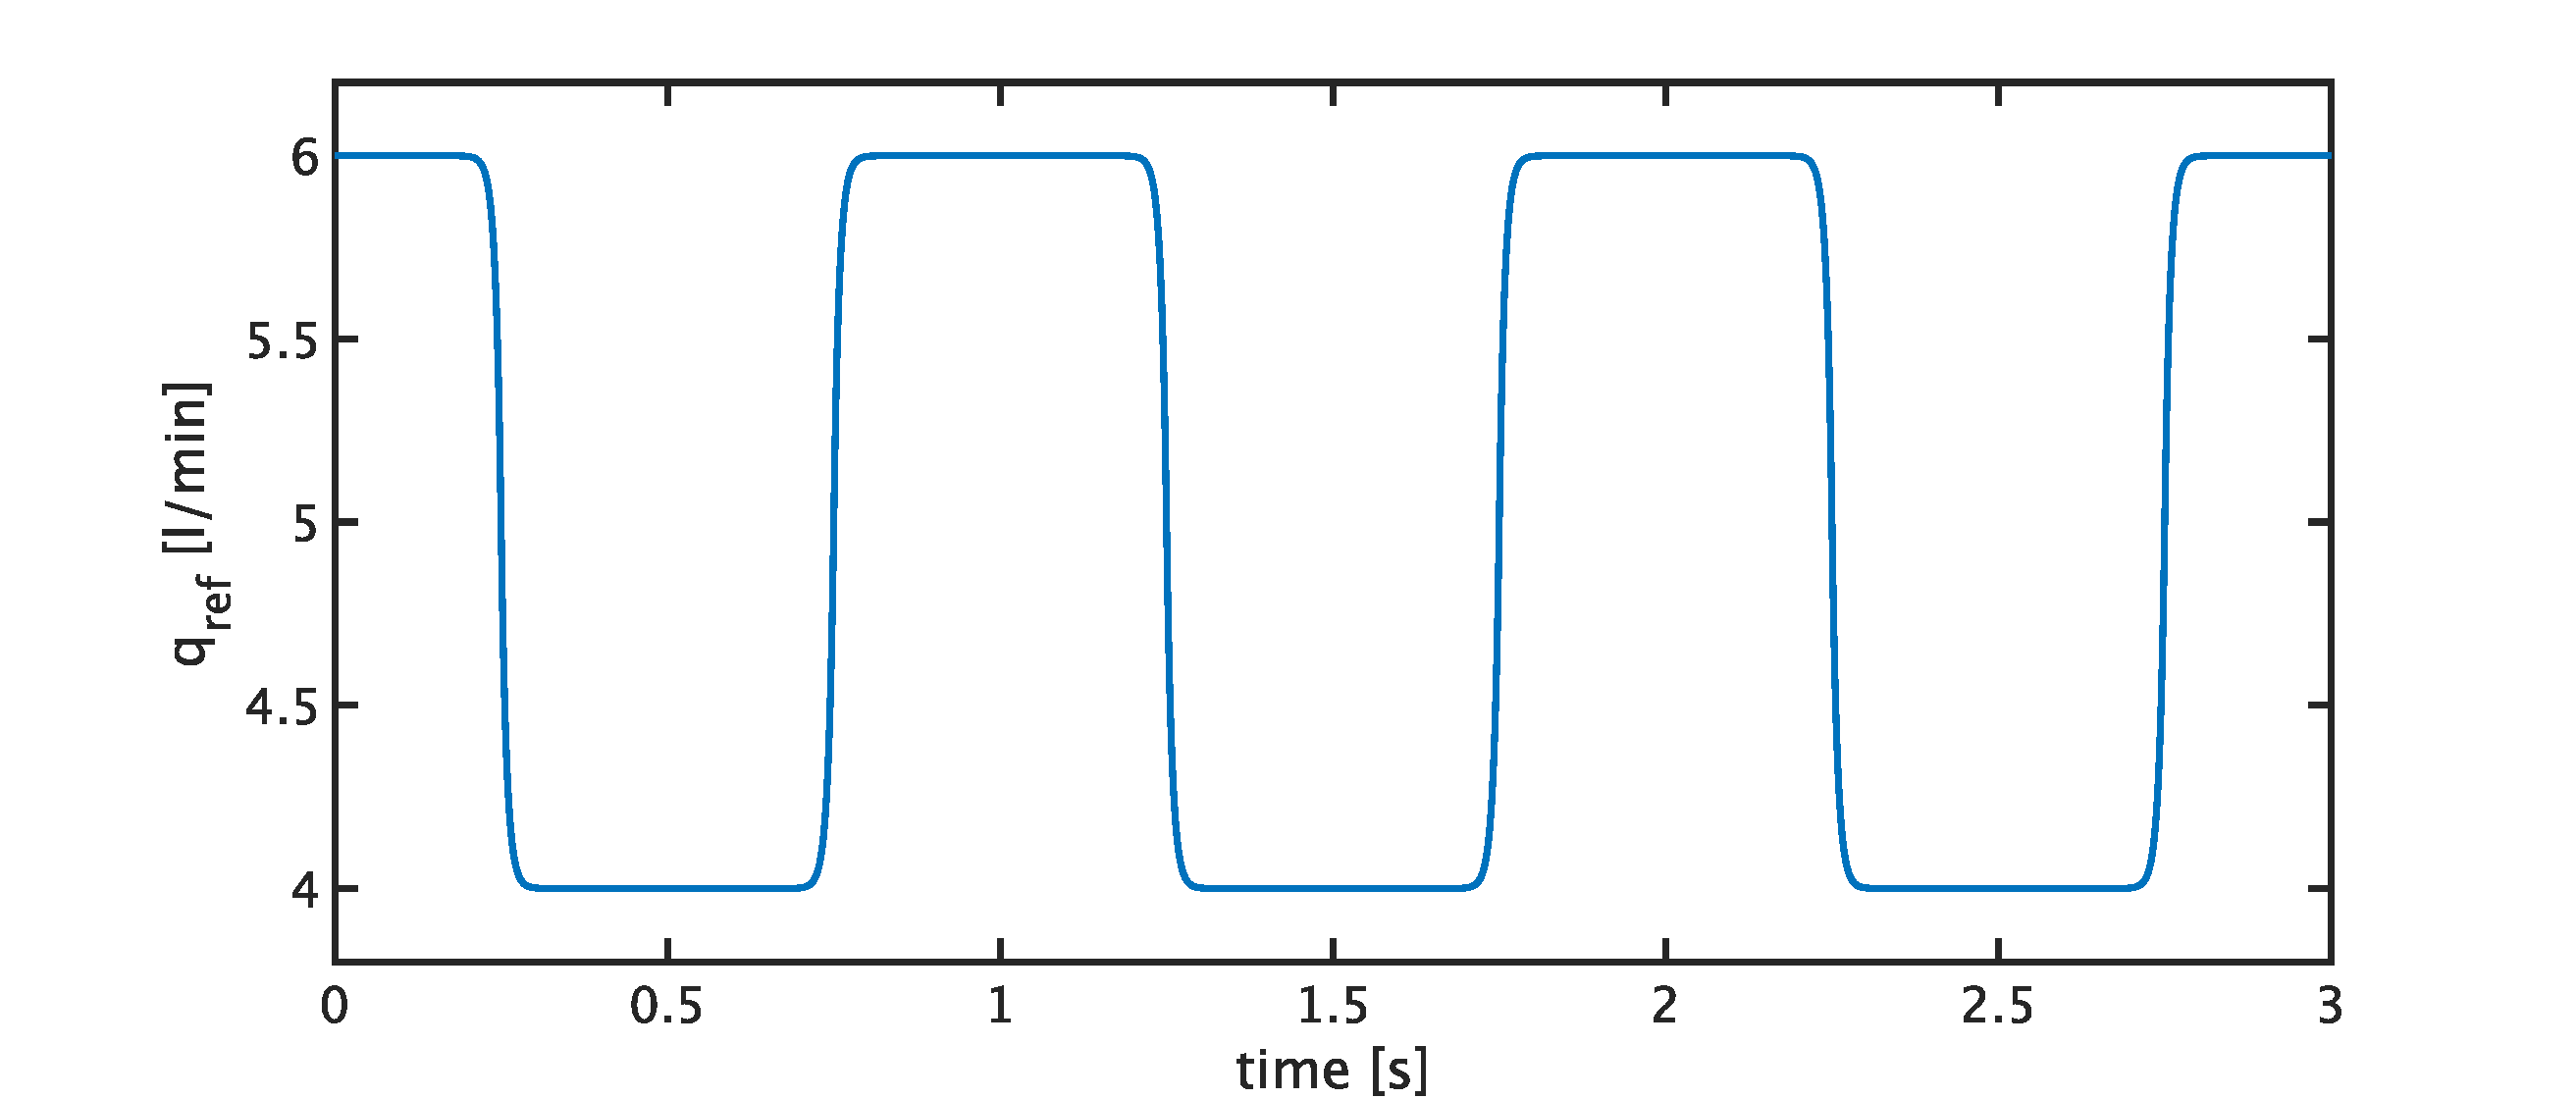
\includegraphics[width=0.95\textwidth]{images/chapt_5/ILC/ref_signal_ILC3.pdf}
  \caption[Smoothed reference signal for ILC tuning]{Three iterations of smoothed reference signal for ILC tuning.}
  \label{fig:ref_signal_ILC3}
\end{figure}
\subsection{Evaluation}
As mentioned above, various cut off frequencies for the Q-Filter of the ILC are tested with the aim of optimizing the ILC's performance and robustness.  \\The test signal for this purpose, is given by repeatedly presenting the reference signal from \figurename~\ref{fig:ref_signal_ILC3} to the system over a duration of $600\,s$. During the first $60\,s$ exclusively PI control is activated. By this, stable system performance at the beginning of ILC control can be ensured. Once the $60\,s$ are up, the trigger signal will set off indications for beginnings of new iterations. From this point, ILC and PI controller are working simultaneously. During the complete test measurement differential pressure is set to $\Delta{p}=40\,mmHg$. Measurements with this setup are performed for cut off frequencies $f_{\mathrm{c}}=20\,Hz$, $f_{\mathrm{c}}=25\,Hz$, $f_{\mathrm{c}}=8\,Hz$ and $f_{\mathrm{c}}=34\,Hz$.
\\\figurename~\ref{fig:pi_to_ilc} exemplifies a sequence of the measurement performed for the Q-Filter set to a cut off frequency of $f_{\mathrm{c}}=20\,Hz$. The segment shows the transition from exclusive PI control to the parallel control structure of PI control and ILC. The upper graph depicts the measured differential pressure at the MCL. The spikes in this curve occur due to varying flow through the blood pump resulting in changing volumes inside the pressure chambers. The middle graph represents the rotational speed values for the actuating variable $v_{\mathrm{act}}$ and the actual velocity of the pump's rotor $v_{\mathrm{vad}}$.

\begin{figure}[ht]
  \centering
  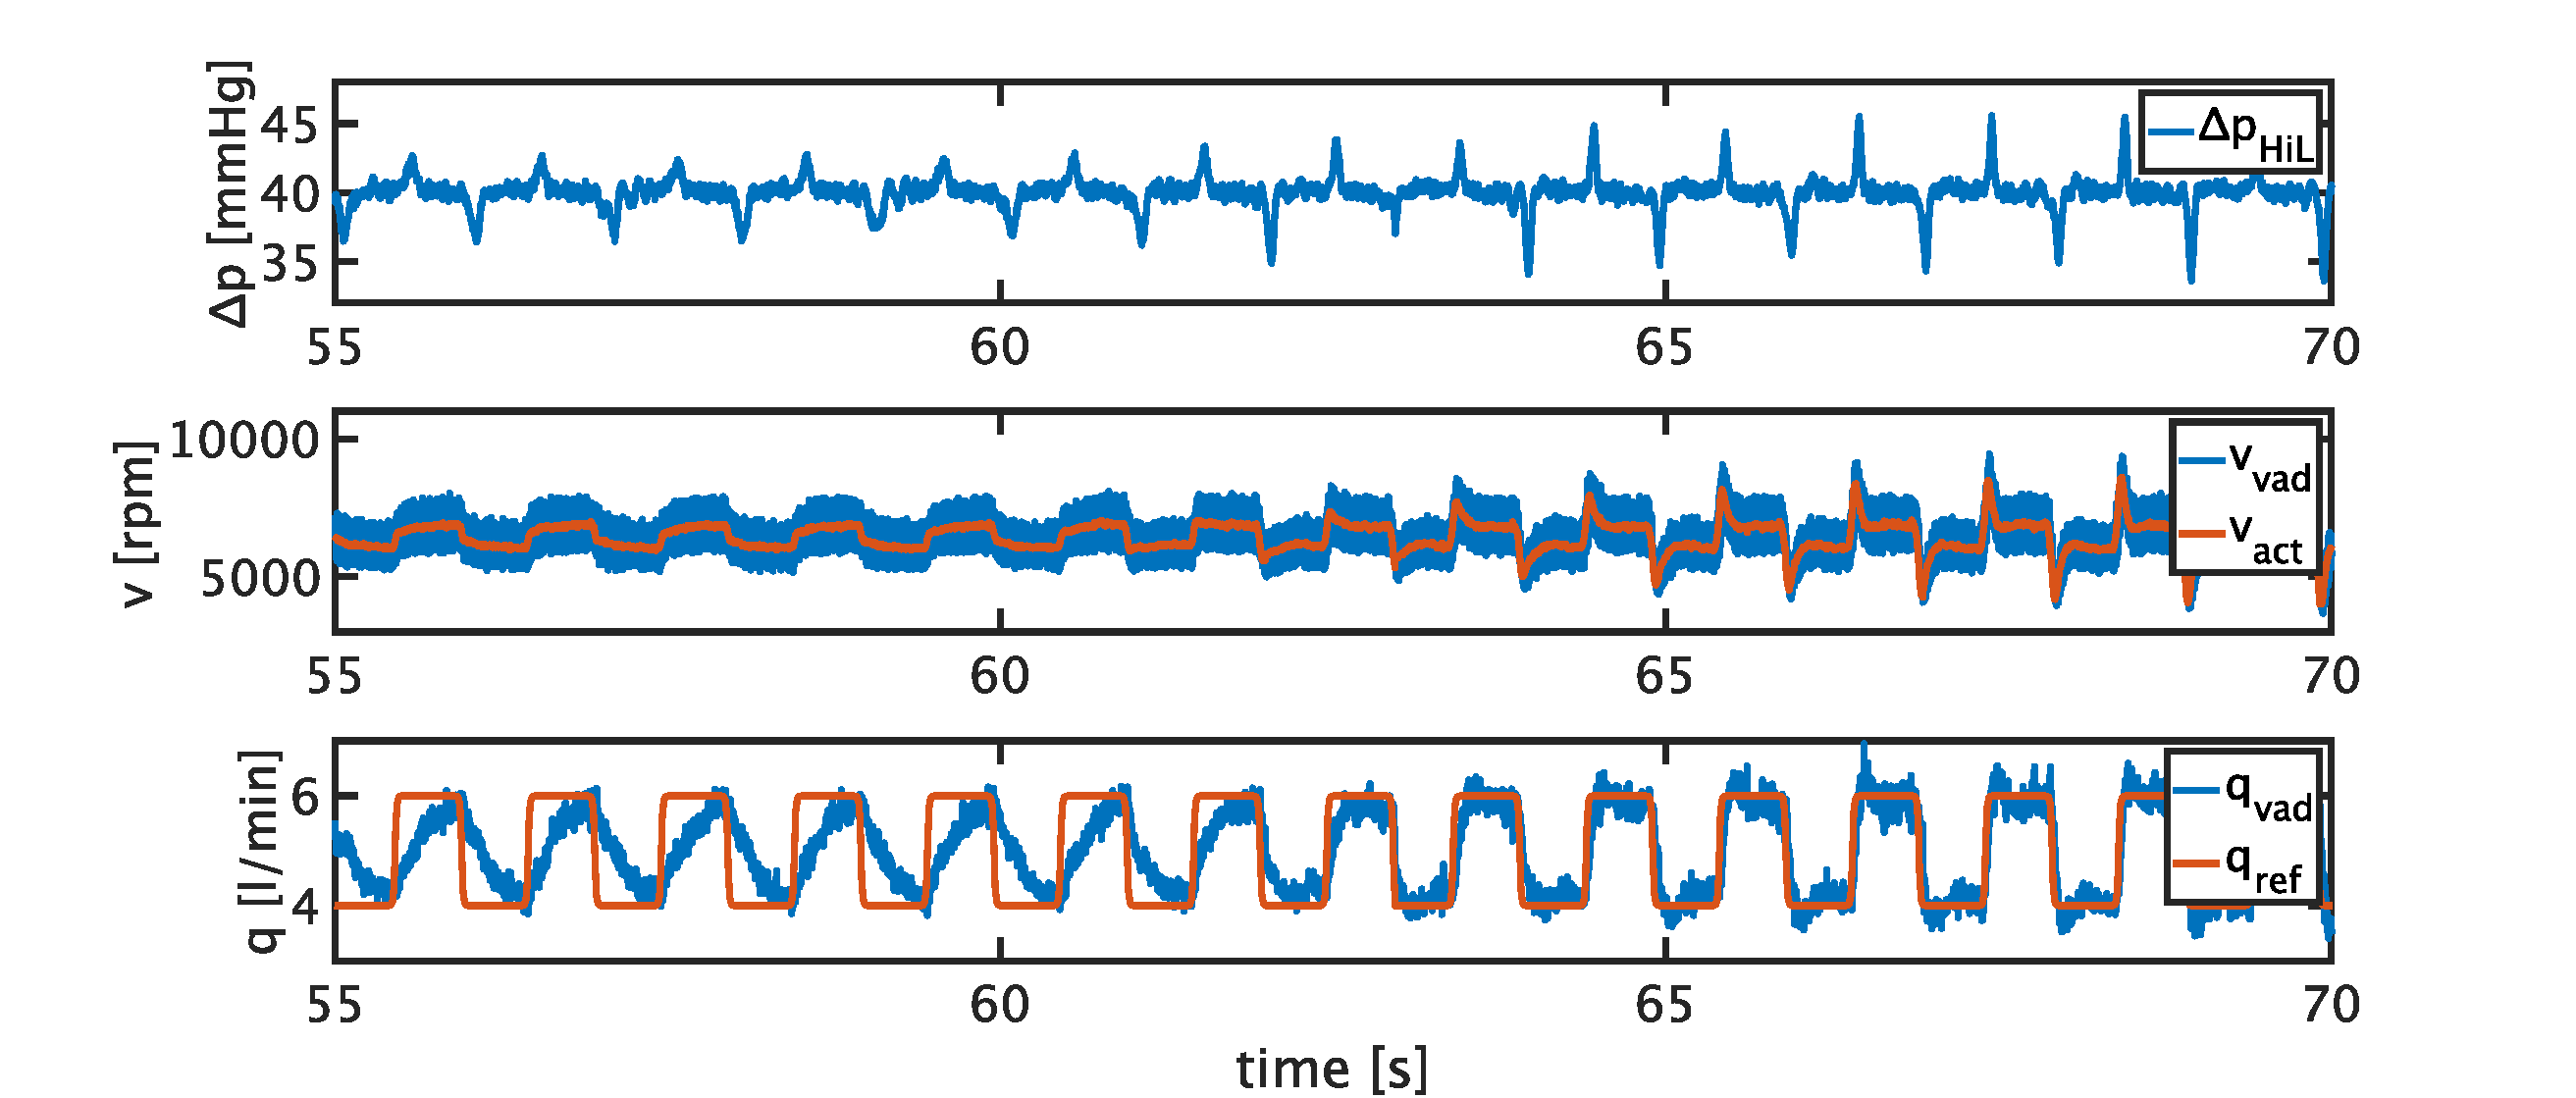
\includegraphics[width=0.95\textwidth]{images/chapt_5/ILC/pi_to_ilc_fc_20.pdf}
  \caption[Test measurement for ILC at cut off frequency $f_{\mathrm{c}}=20\,Hz$]{Test measurement for ILC at cut off frequency $f_{\mathrm{c}}=20\,Hz$.  Top: differential pressure value of the MCL. Middle: actuating variable and measured rotational speed of the VAD. Bottom: targeted flow trajectory and measured flow through the VAD.}
  \label{fig:pi_to_ilc}
\end{figure}
The bottom graph of \figurename~\ref{fig:pi_to_ilc} depicts the reference flow trajectory $q_{\mathrm{ref}}$ and the measured flow $q_{\mathrm{vad}}$ that is conveyed by the VAD. Looking at this curve, it can be seen that by solely using the PI controller (corresponding to $55\,s$ to $60\,s$ of the graph), the flow through the VAD cannot be adjusted fast enough and thus the reference trajectory cannot be followed successfully. However, from the onset of the ILC at about $60\,s$, it can be seen that the measured flow continues to adapt to the given reference flow within a few iterations.
\\While the system shows stable behavior over the complete measurement time for a cut off frequency of $f_{\mathrm{c}}=20\,Hz$, in case of $f_{\mathrm{c}}=34\,Hz$ the system shows oscillatory behavior. \figurename~\ref{fig:pi_to_ilc_fc_34} depicts part of the measurement for a cut off frequency set to $f_{\mathrm{c}}=34\,Hz$.
\begin{figure}[ht]
  \centering
  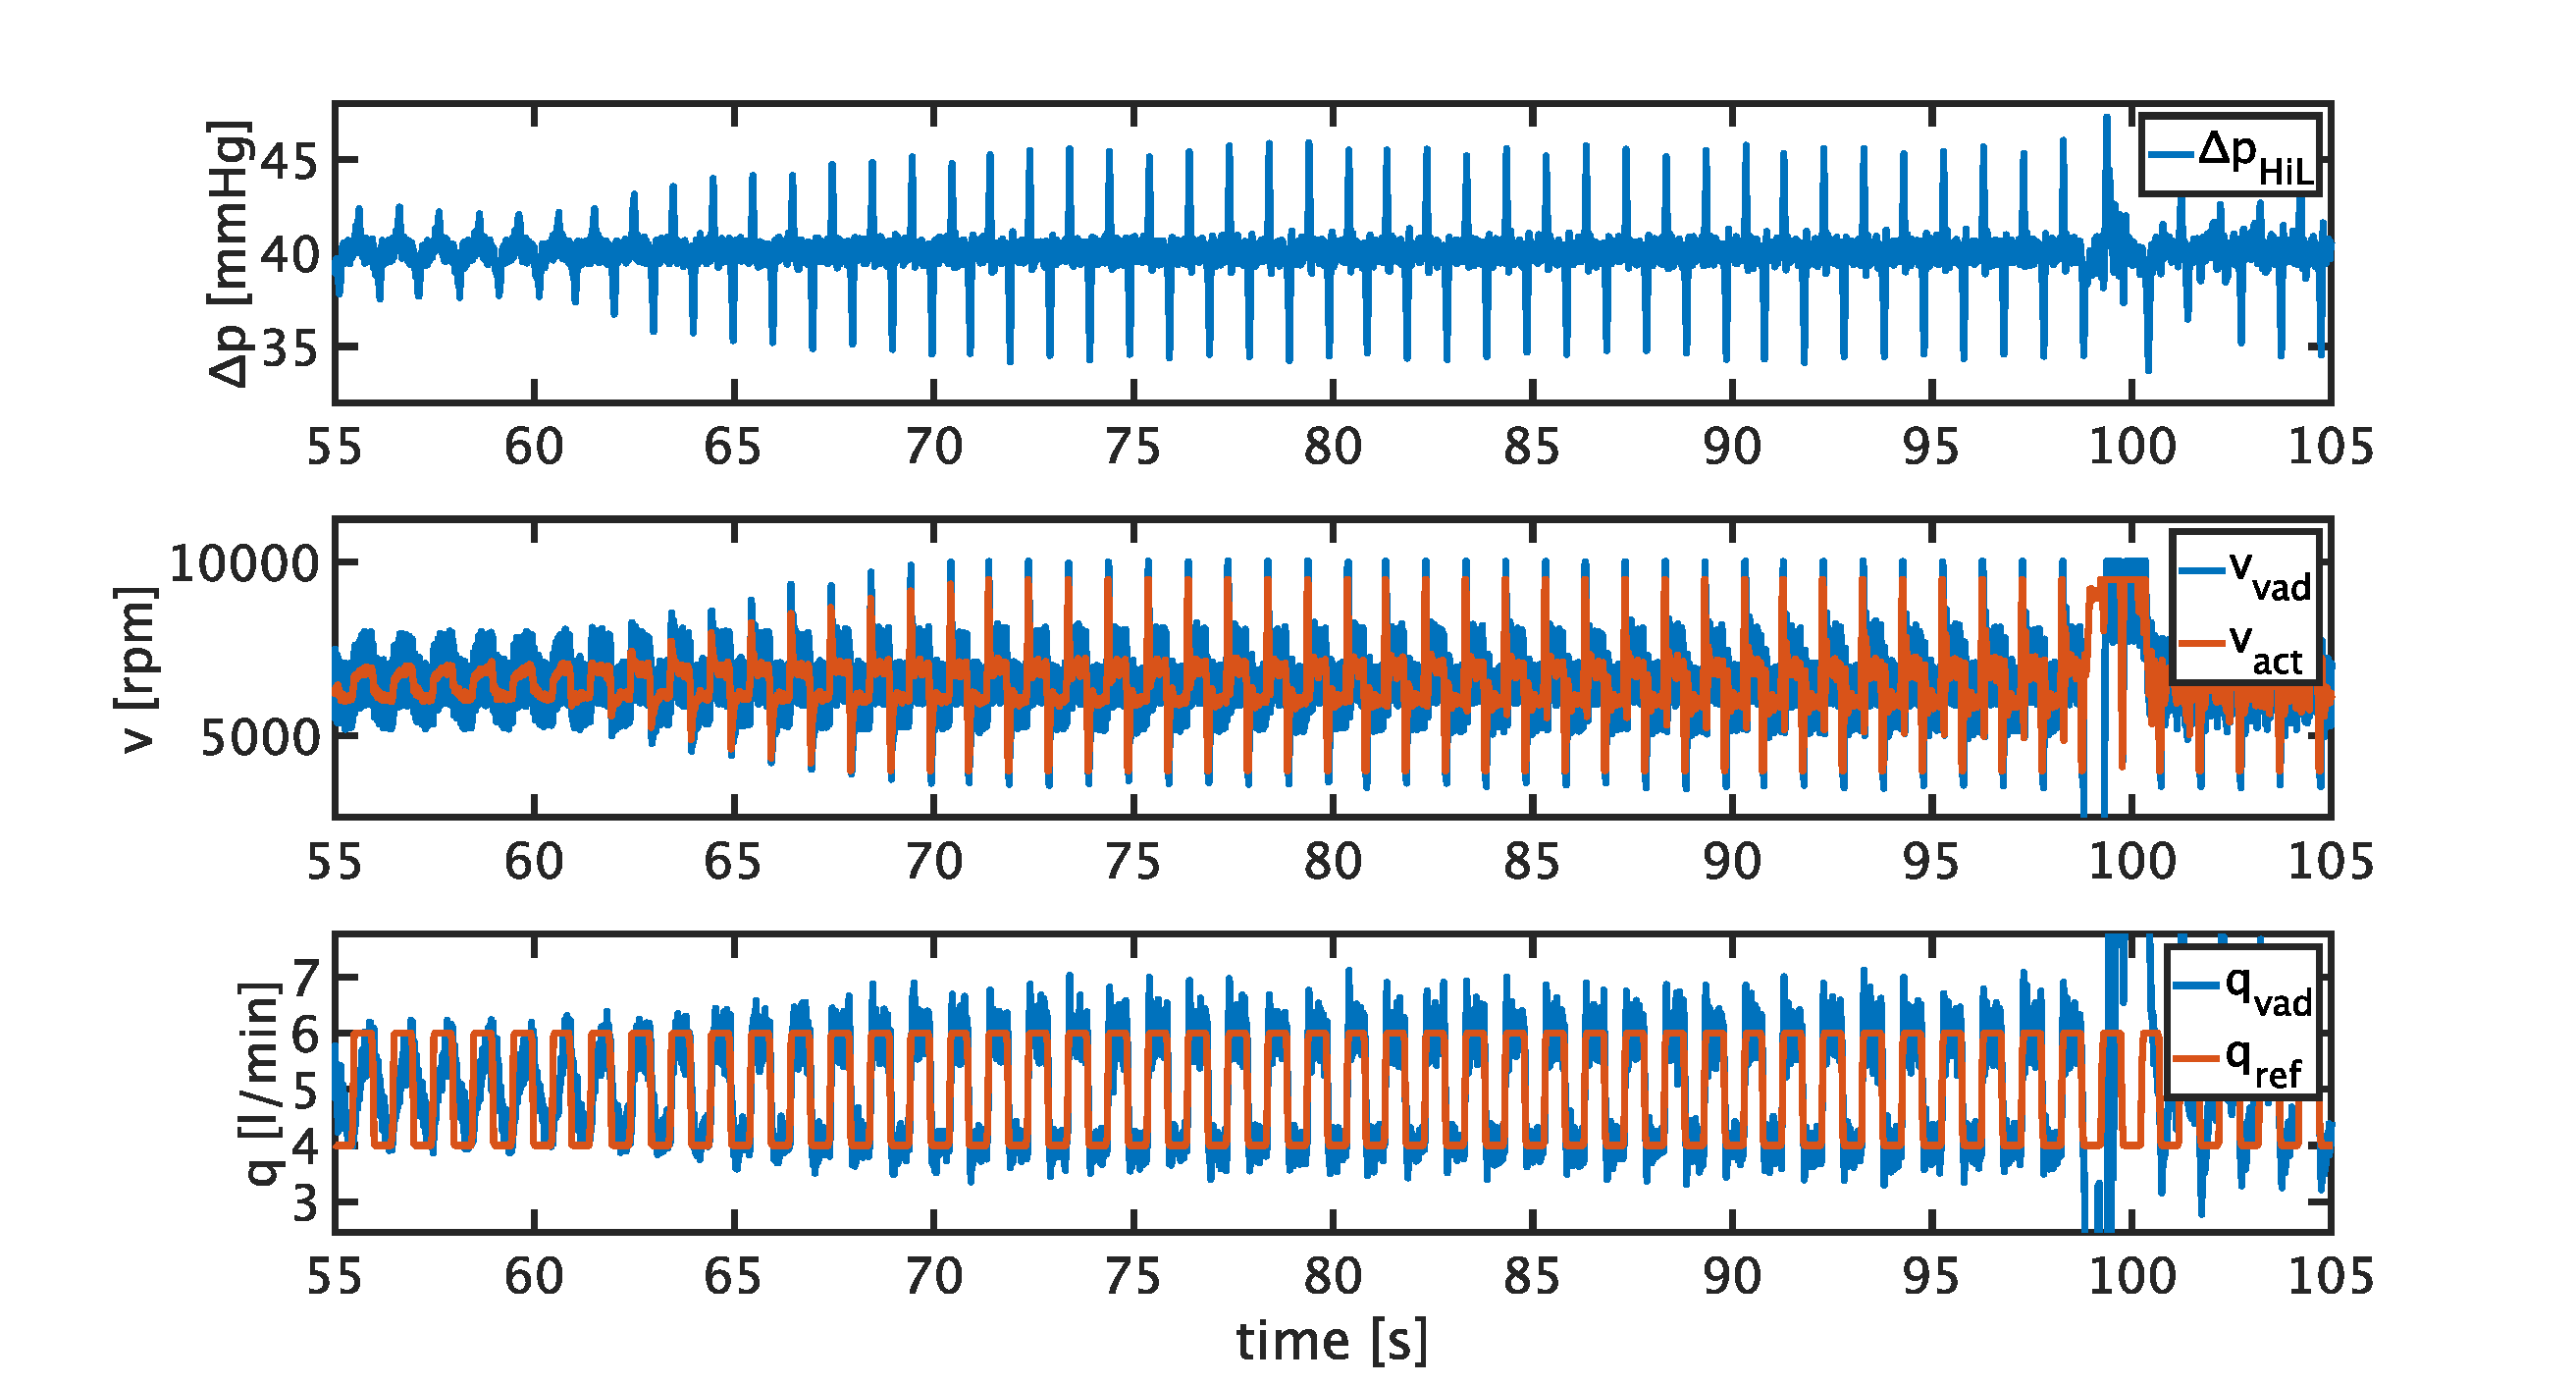
\includegraphics[width=0.95\textwidth]{images/chapt_5/ILC/pi_to_ilc_fc_34.pdf}
  \caption[Test measurement for ILC at cut off frequency $f_{\mathrm{c}}=34\,Hz$]{Test measurement for ILC at cut off frequency $f_{\mathrm{c}}=34\,Hz$. Top: differential pressure value of the MCL. Middle: actuating variable and measured rotational speed of the VAD. Bottom: targeted flow trajectory and measured flow through the VAD.}
  \label{fig:pi_to_ilc_fc_34}
\end{figure}
\\The structure is the same as for \figurename~\ref{fig:pi_to_ilc}. However, in this case, looking at the middle graph it is evident that with each additional ILC iteration the actuation variable $v_{\mathrm{act}}$ rises further towards its saturation values $4000\,rpm$ and $9000\,rpm$. This ultimately leads to the pump's rotor to stop, due to abrupt changes in speed and flow at approximately $98\,s$ measurement time.
\\Behavior of the system for a cut off frequency set to $f_{\mathrm{c}}=25\,Hz$ ,as shown in \figurename~\ref{fig:pi_to_ilc_fc_25}, is similar to behavior with $f_{\mathrm{c}}=34\,Hz$. The oscillatory system behavior again results in the pump's rotor to stop at approximately $96\,s$.
\begin{figure}[ht]
  \centering
  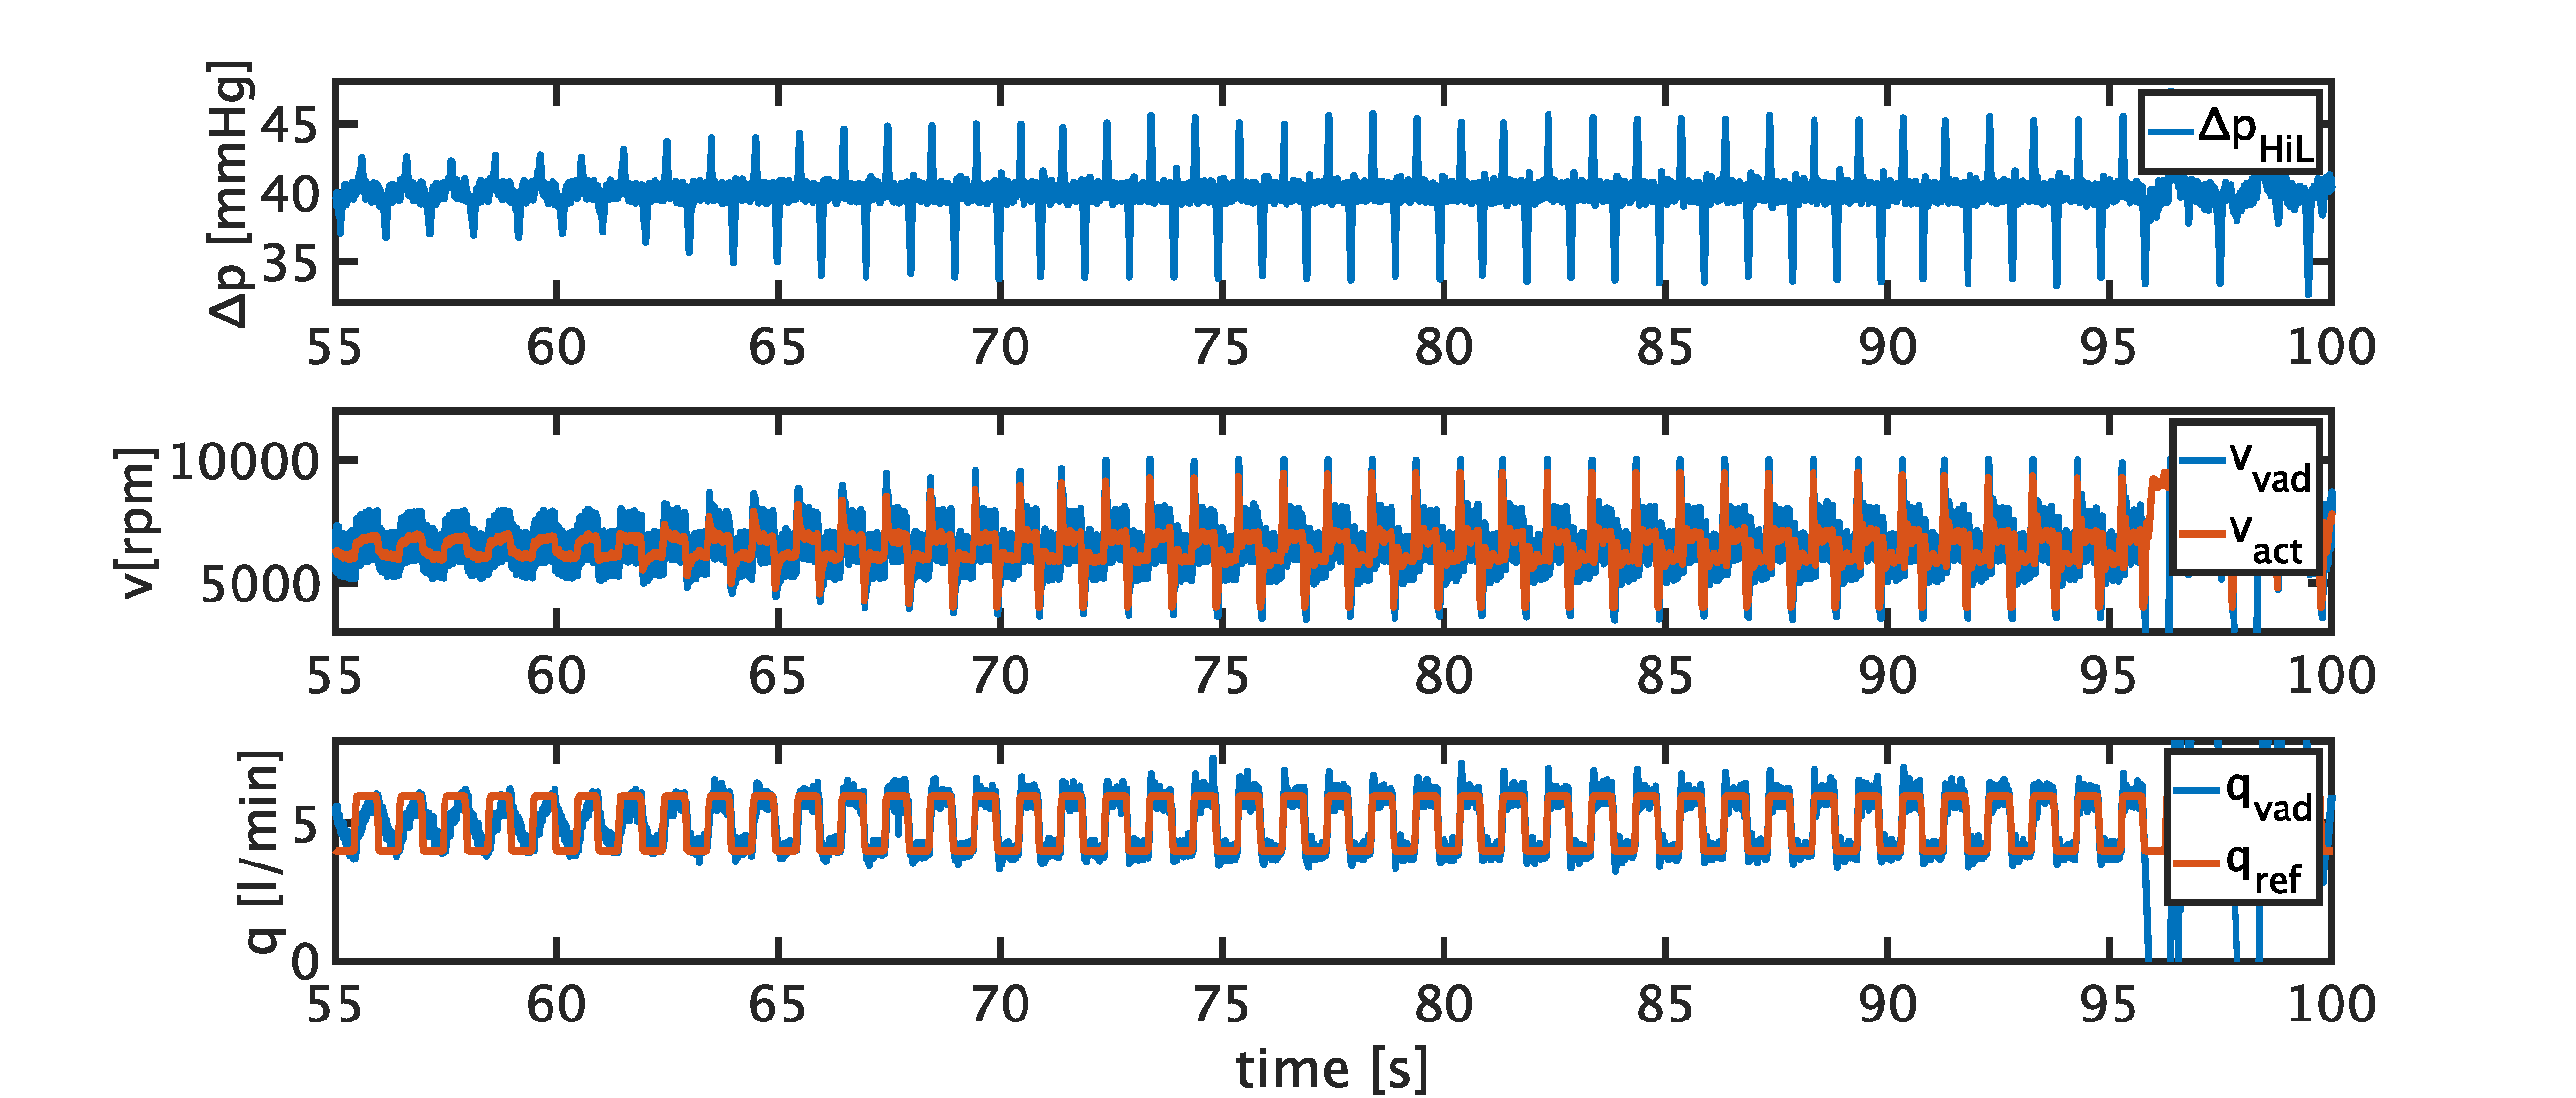
\includegraphics[width=0.95\textwidth]{images/chapt_5/ILC/pi_to_ilc_fc_25.pdf}
  \caption[Test measurement for ILC at cut off frequency $f_{\mathrm{c}}=25\,Hz$]{Test measurement for ILC at cut off frequency $f_{\mathrm{c}}=25\,Hz$. Top: differential pressure value of the MCL. Middle: actuating variable and measured rotational speed of the VAD. Bottom: targeted flow trajectory and measured flow through the VAD.}
  \label{fig:pi_to_ilc_fc_25}
\end{figure}
\\The measurement with $f_{\mathrm{c}}=8\,Hz$ as cut off frequency of the Q-Filter shows stable behavior over the complete measurement time, similar to the measurement performed with $f_{\mathrm{c}}=20\,Hz$.
\\In order to determine which cut off frequency is most suited for the ILC implementation the RMSE values of the iterations for each of the measurements are compared to another. \figurename~\ref{fig:RMSE_compare_ILC3_fc} depicts the RMSE of each measurement as a function of the iteration for the first 39 iterations of the ILC. The figure also represents the RMSE value of the exclusive performing PI controller in form of the first iteration value:
\begin{equation}
  RMSE_{PI}=RMSE(1)\approx 0.85\,l/min
\end{equation}
It is evident that the curves for $f_{\mathrm{c}}=25\,Hz$ and $f_{\mathrm{c}}=35\,Hz$ show abrupt increases in RMSE for the iterations when the pump stopped. Due to this instable behavior these cut off frequencies are not suitable for ILC implementation.
\begin{figure}[ht]
  \centering
  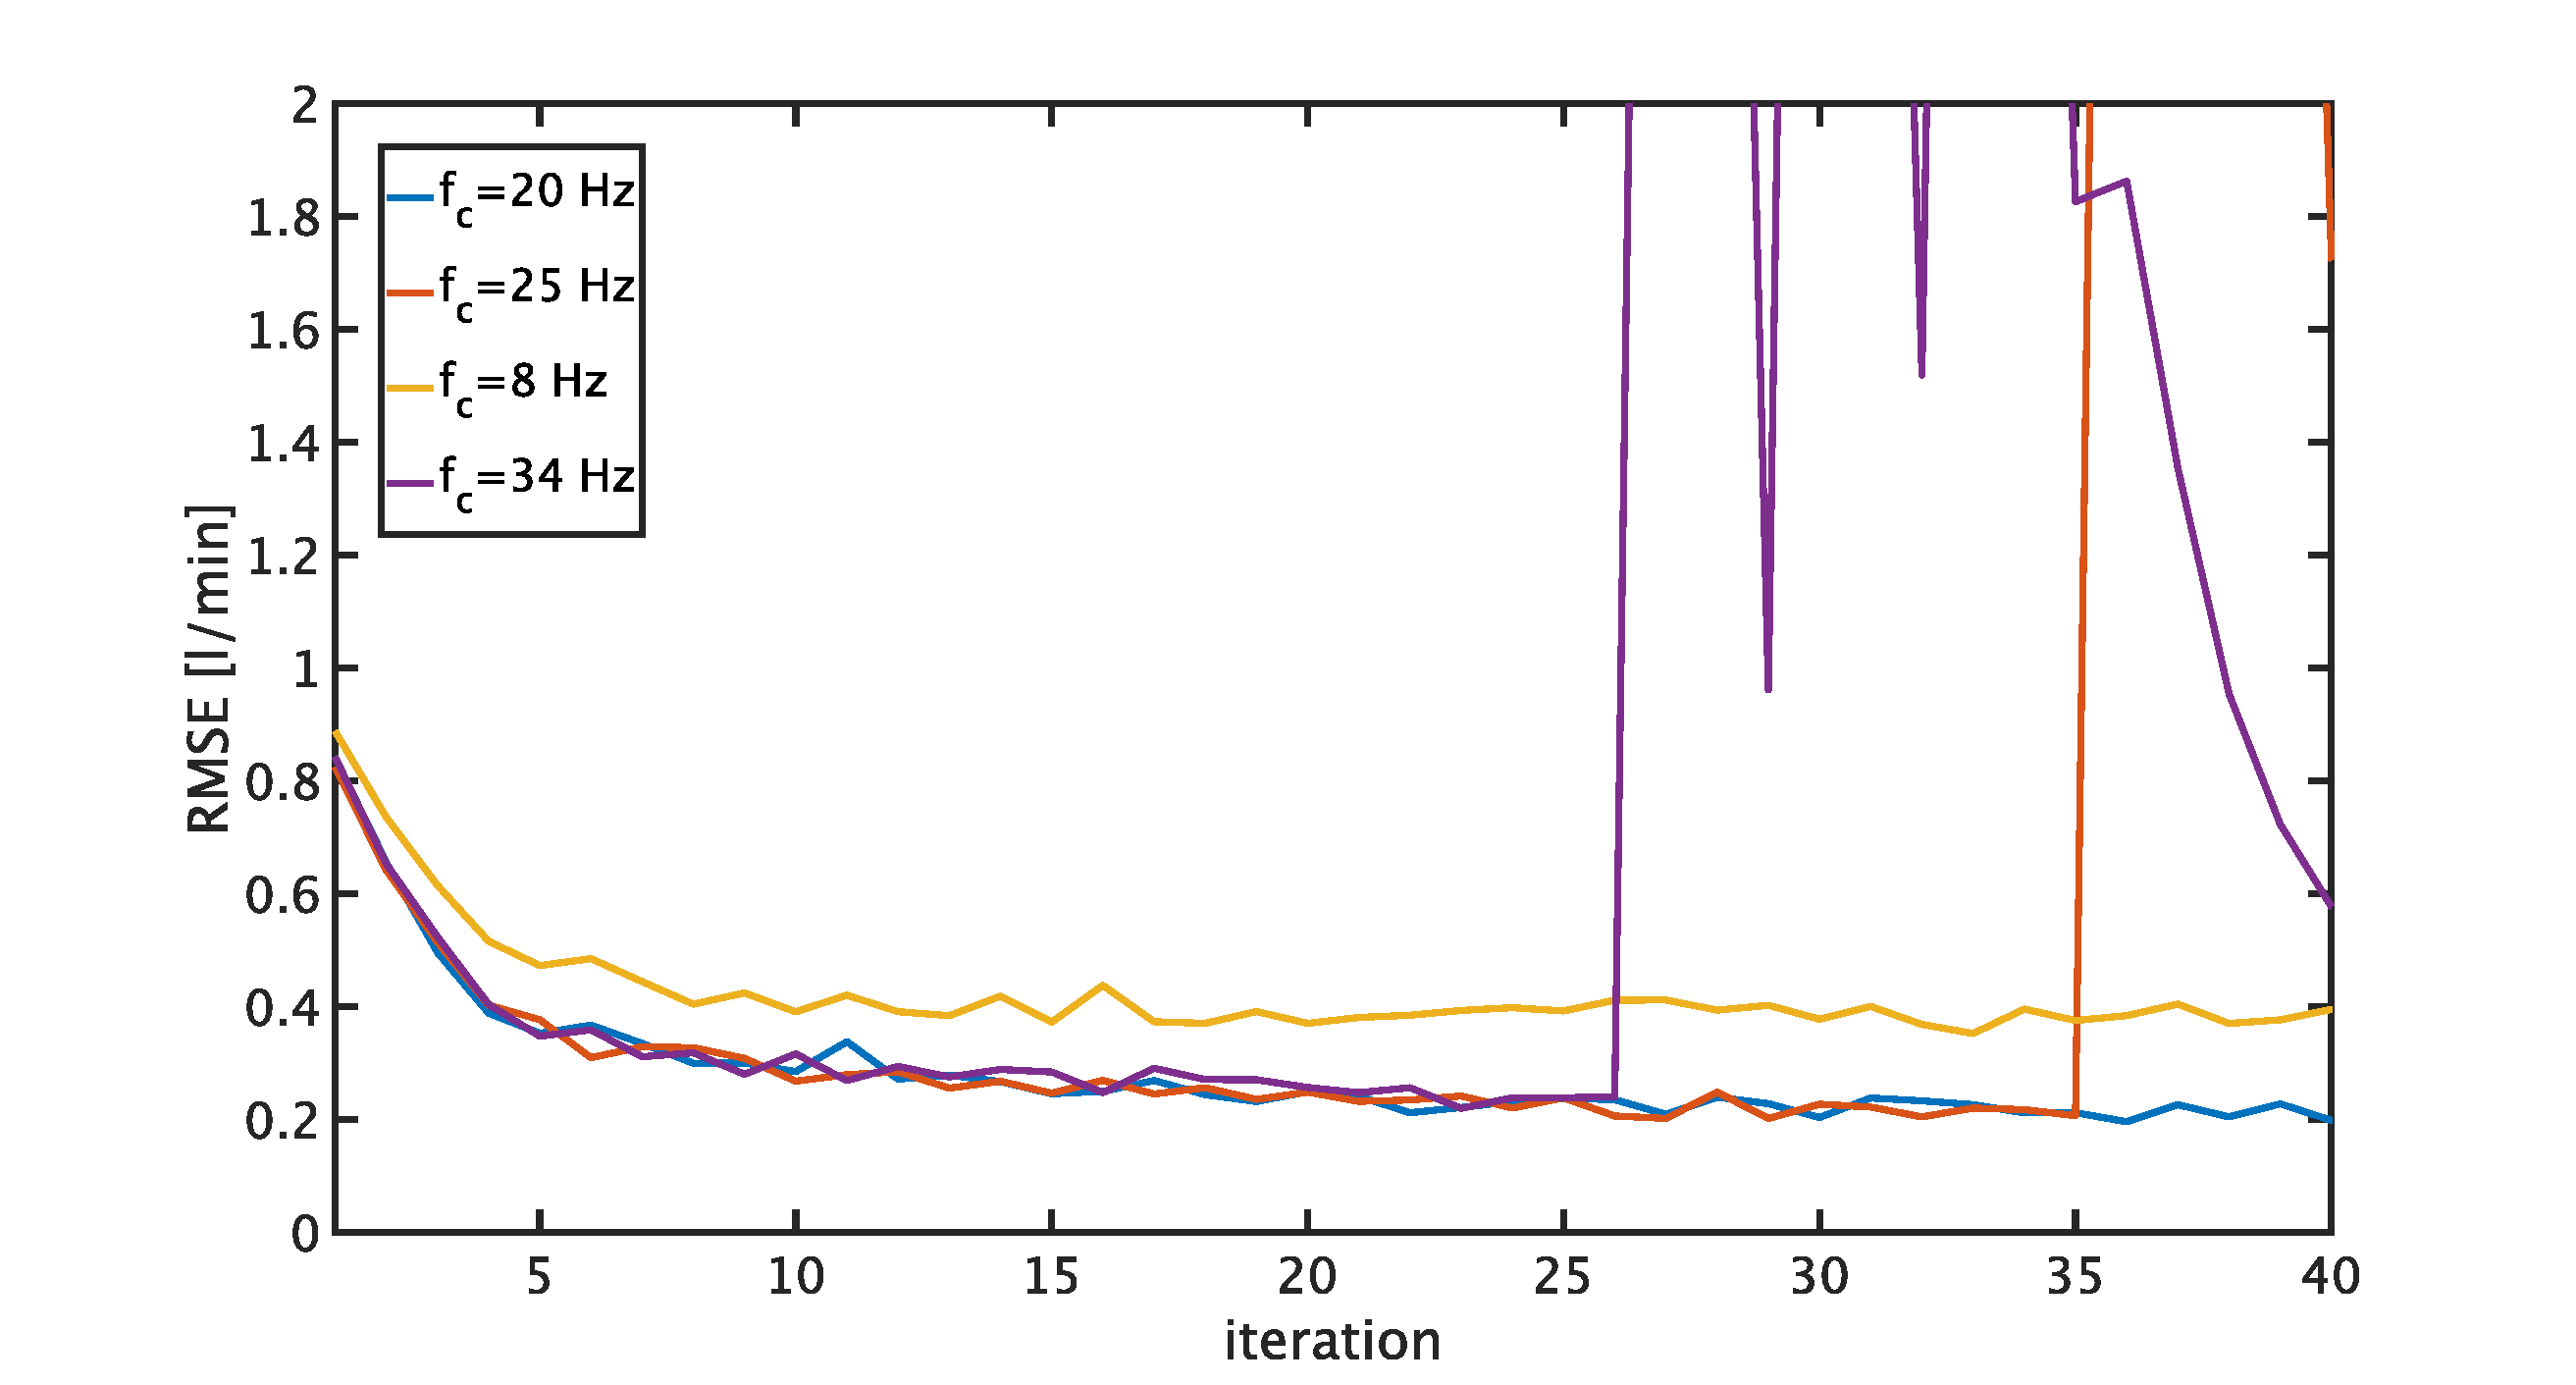
\includegraphics[width=\textwidth]{images/chapt_5/ILC/RMSE_compare_ILC3_fc.pdf}
  \caption[Comparison of RMSE values for different cut off frequencies of ILC Q-Filter]{Comparison of RMSE values for different cut off frequencies of ILC Q-Filter.}
  \label{fig:RMSE_compare_ILC3_fc}
\end{figure}
\\Comparing the RMSE values of the $39^{th}$ iteration of the other two frequencies it is obvious that performance of the ILC with Q-filter cut off frequency at $f_{\mathrm{c}}=20\,Hz$ with
\begin{equation}
  RMSE_{\mathrm{f_{\mathrm{c}}=20\,Hz}}(39)=0.1984\,l/min
\end{equation}
is higher than for $f_{\mathrm{c}}=8\,Hz$ with
\begin{equation}
  RMSE_{\mathrm{f_{\mathrm{c}}=8\,Hz}}(39)=0.3951\,l/min.
\end{equation}
Therefore, the cut off frequency of the Q-Filter in all following measurements will be set to $f_{\mathrm{c}}=20\,Hz$.

As these measurements only took into account a differential pressure value of $\Delta{p}=40mmHg$ the ILC with the optimized Q-Filter cut off frequency is tested at pressure levels in in equal steps of $20\,mmHg$ between $\Delta{p}=20mmHg$ and $\Delta{p}=80\,mmHg$ to ensure stable system behavior in all operating points. For this the same measurement as before is executed.
\\A comparison of the RMSE values over all iterations of the ILC for the four differential pressure levels is depicted in \figurename~\ref{fig:RMSE_compare_operating_points}. The course of the RMSE values of all four measurements indicate stable system behavior. With values of approximately $0.3\, l/min$ the RMSE of the other operating points is only slightly higher than of the $40\,mmHg$ operating point with an RMSE of approximately $0.2\,l/min$. Therefore, the implemented ILC is suitable for all of the tested operating points.

\begin{figure}[ht]
  \centering
  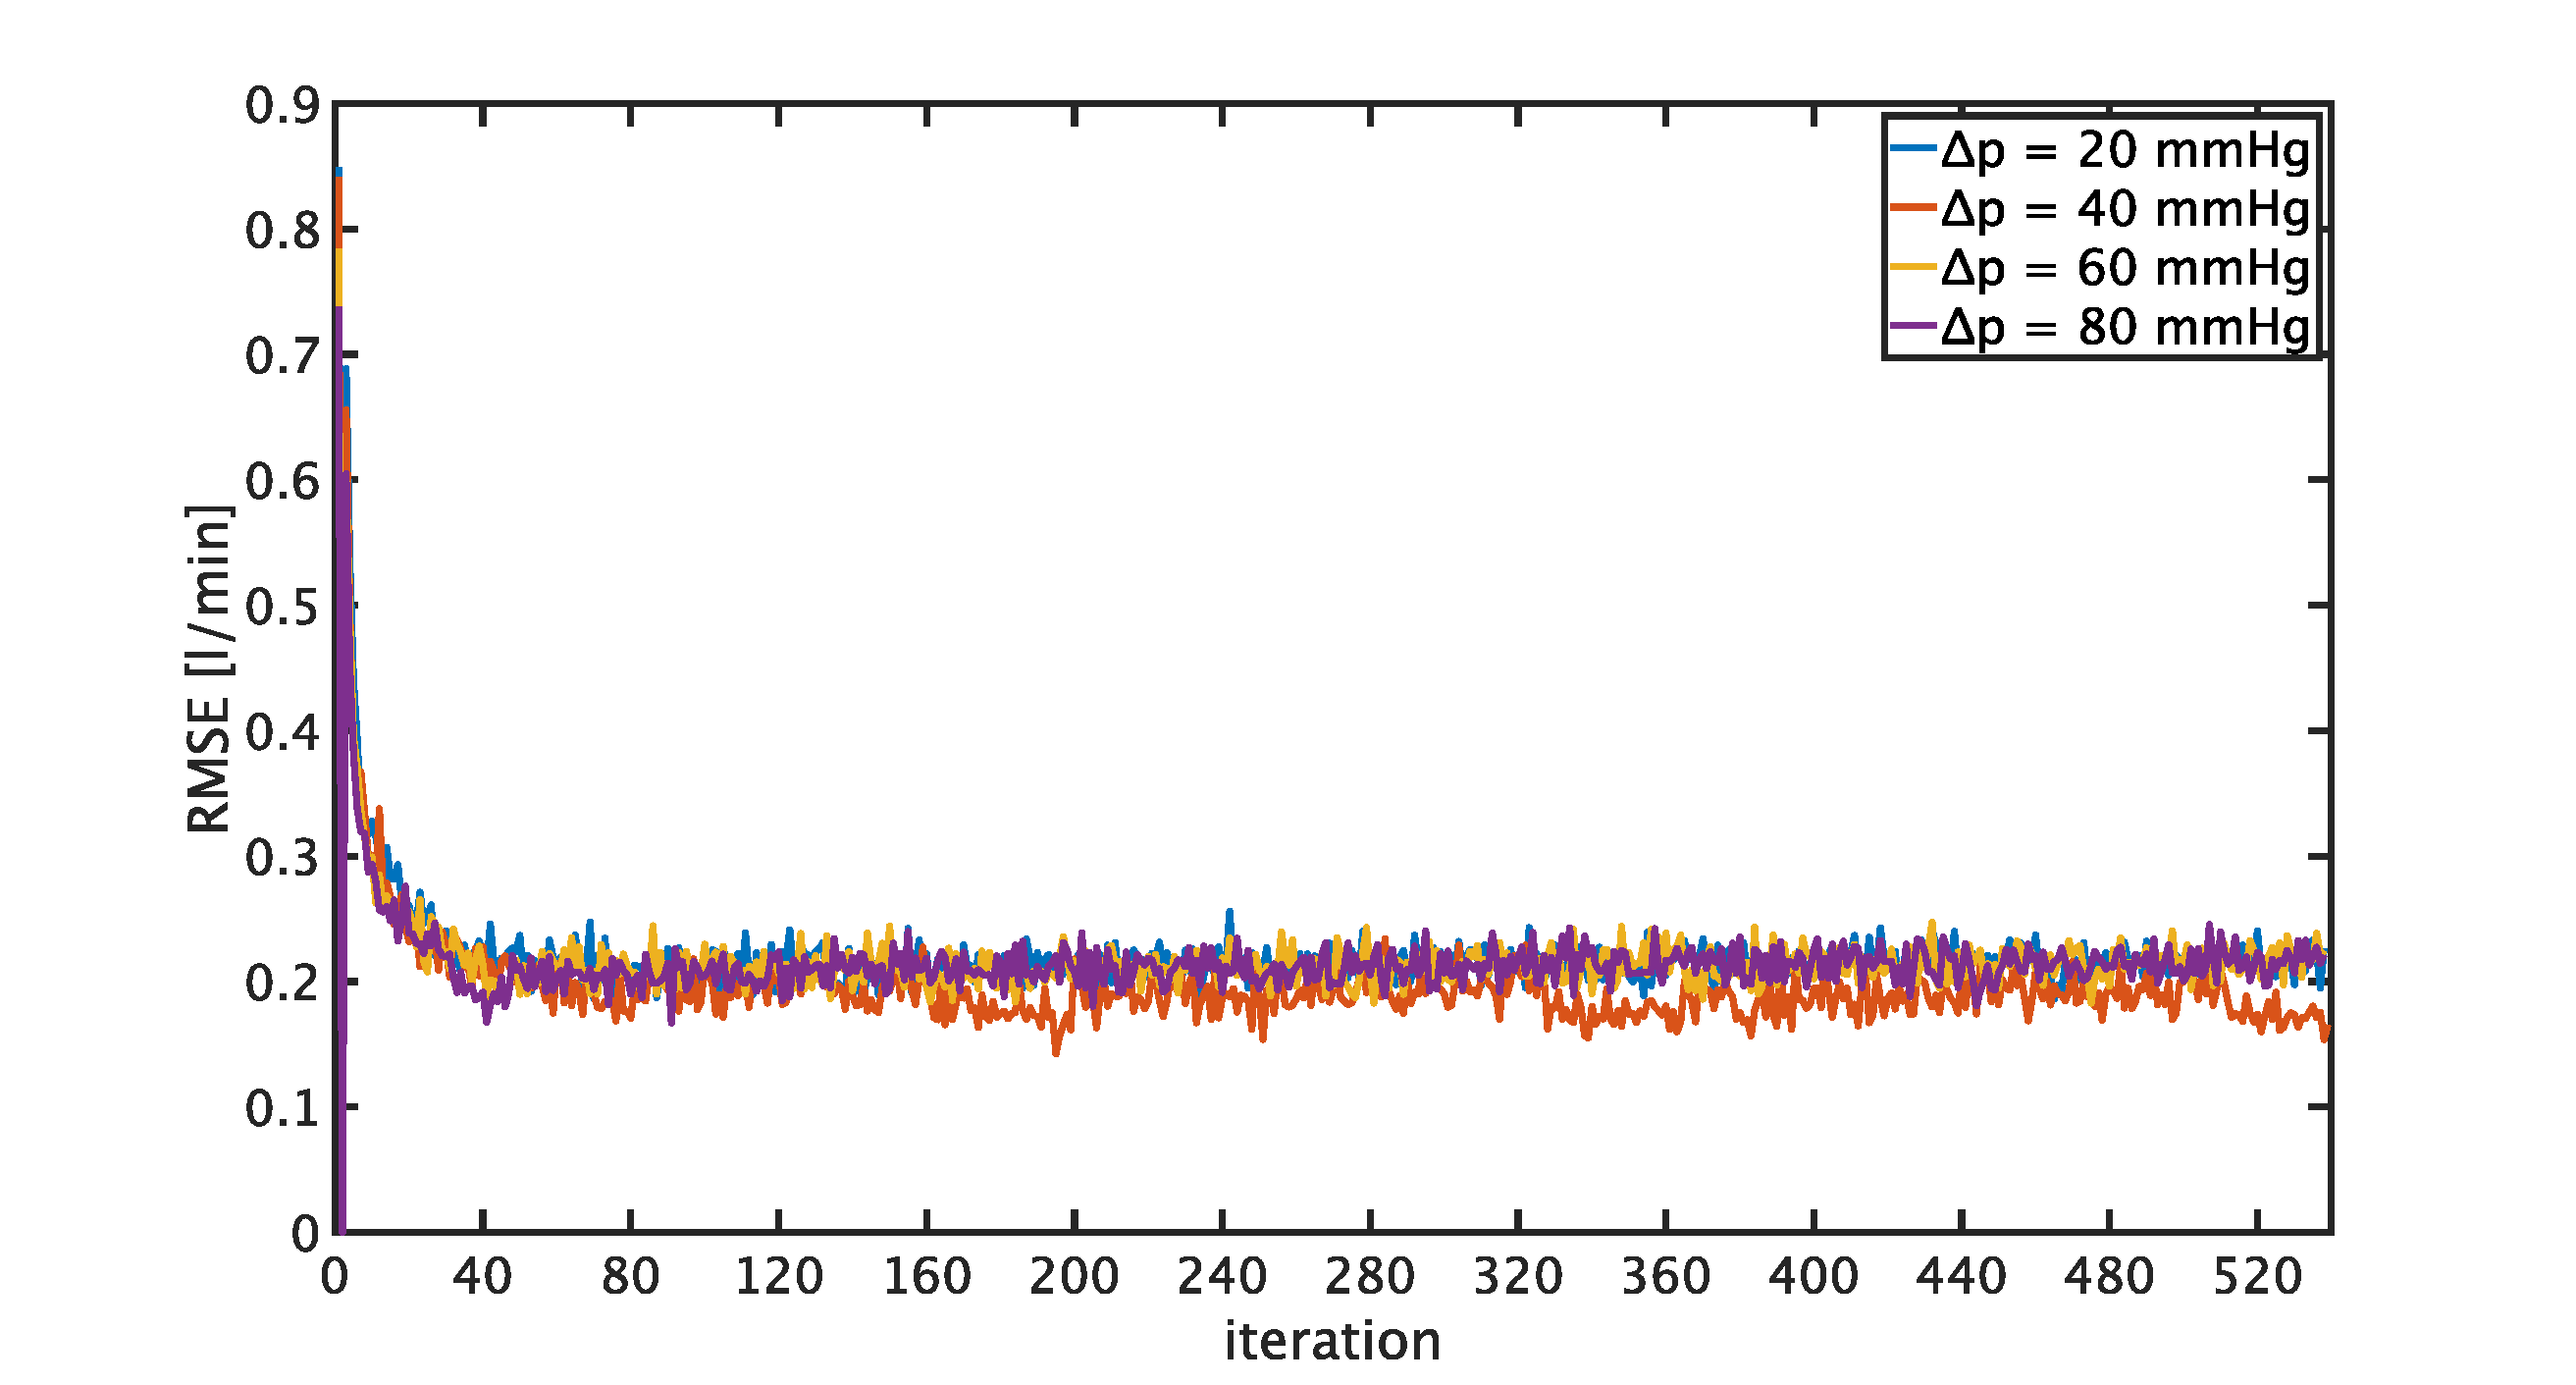
\includegraphics[width=\textwidth]{images/chapt_5/ILC/RMSE_compare_operating_points.pdf}
  \caption[Comparison of RMSE values of the ILC at different differential pressure operating points]{Comparison of RMSE values of the ILC at different differential pressure operating points.}
  \label{fig:RMSE_compare_operating_points}
\end{figure}
\section{Iterative Learning Control with repeating disturbance}

The ILC implemented in the previous section was tested and optimized under idealized conditions without being influenced by any disturbances. Since in real use, the VAD is exposed to disturbances by pressure changes due to the beating of the heart this section aims to include this influence into the measurements through usage of the circulatory system simulator's functionality to simulate the heart beat including anticipated pressure changes.
%\subsection{Design and Implementation}

Initially, only repeating disturbances are taken into account as the standard P-type ILC used is only setup to compensate these.
The MCL will be used to introduce the setup to a disturbance in form of heart beats at a constant heart rate. Including the influence of the heart beat as a disturbance requires changing the trigger signal from a manually programmed one to using the start of each heart beat as the trigger of new iterations.
\subsection{Reference trajectories}\label{ref_traject}
Testing of the ILC subjected to repeating disturbances is performed for several reference flow trajectories. These are generated using Matlab and are selectable during runtime via ControlDesk through the use of an indicator variable.

As a first reference, the flow is set to a constant value of $q_{\mathrm{ref}}=5\,l/min$. By this, the controller's ability to balance out the pressure fluctuations during a heart beat is tested.
\\The second signal, which is used as a reference trajectory, is a sinusoidal signal that oscillates around a value of $4\, l/min$, has a maximum value of $5\, l/min$ and a minimum value of $3\, l/min$. One iteration of this signal is set to $1\,s$, matching a $60\,bpm$ heart rate. The signal course is depicted in \figurename~\ref{fig:ref_sine}.
\begin{figure}[ht]
  \centering
  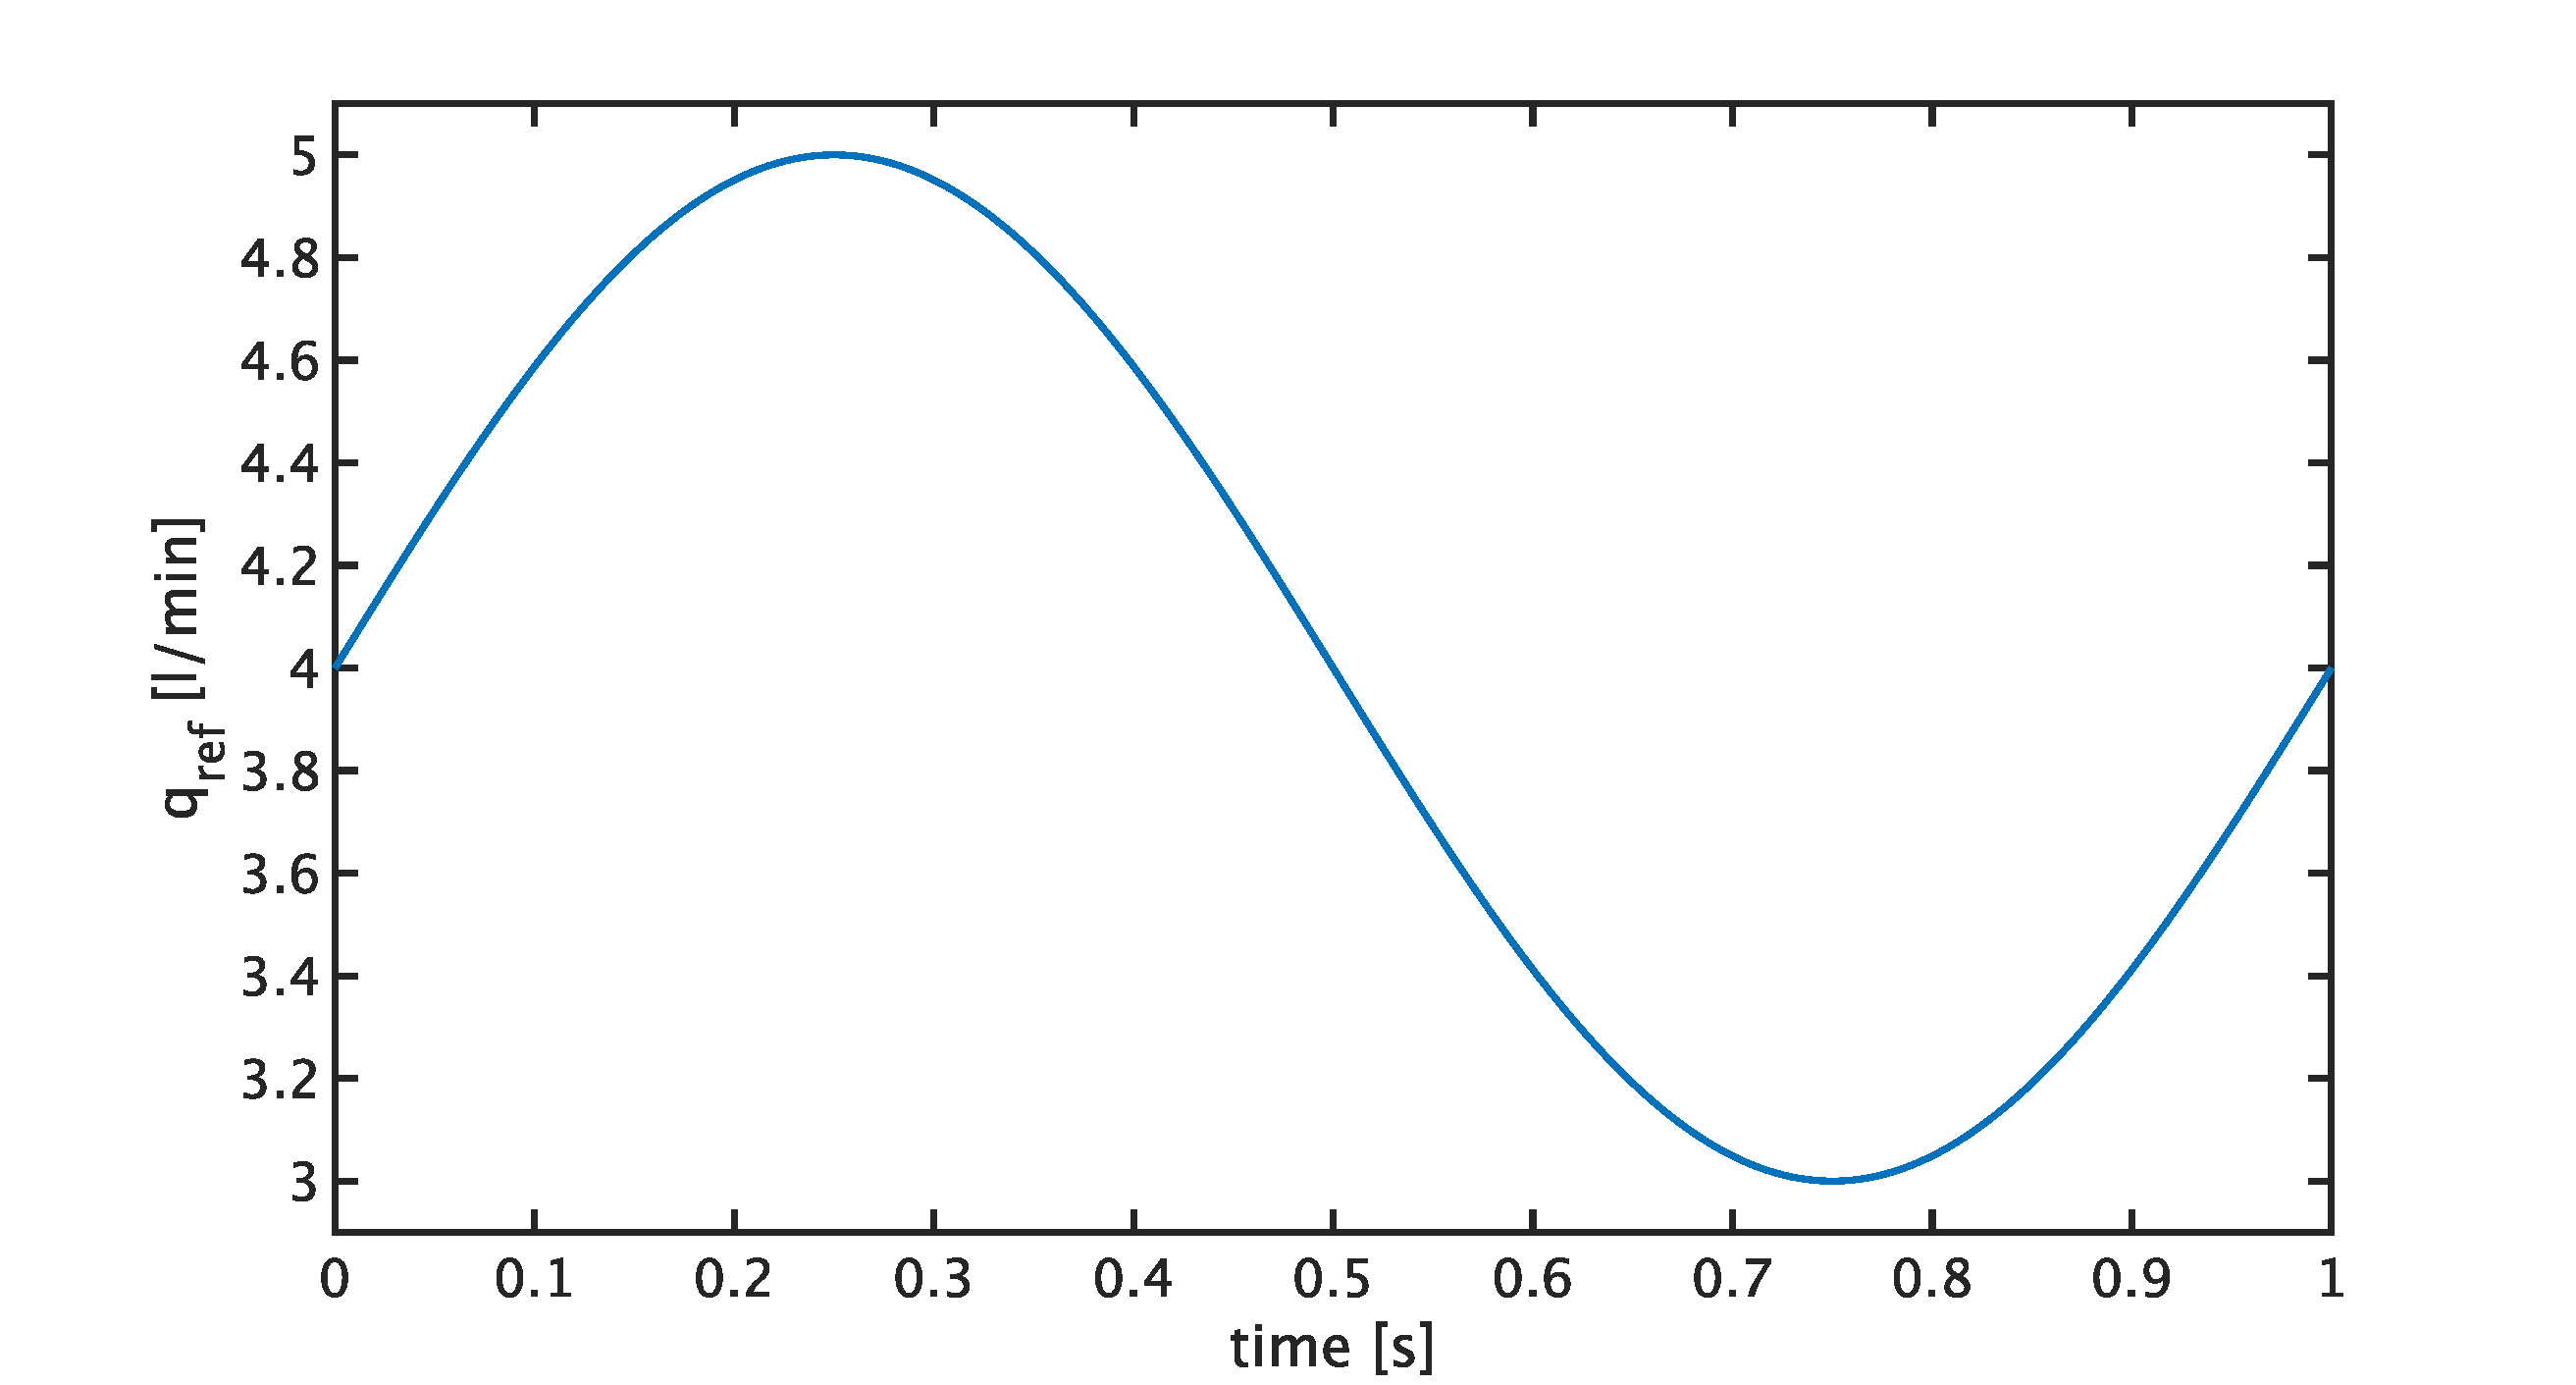
\includegraphics[width=0.95\textwidth]{images/chapt_5/ILC/ref_sine.pdf}
  \caption[Sinusoidal reference signal]{Sinusoidal reference signal.}
  \label{fig:ref_sine}
\end{figure}

% \begin{figure}[ht]
%   \centering
%   \subfloat[]
%   {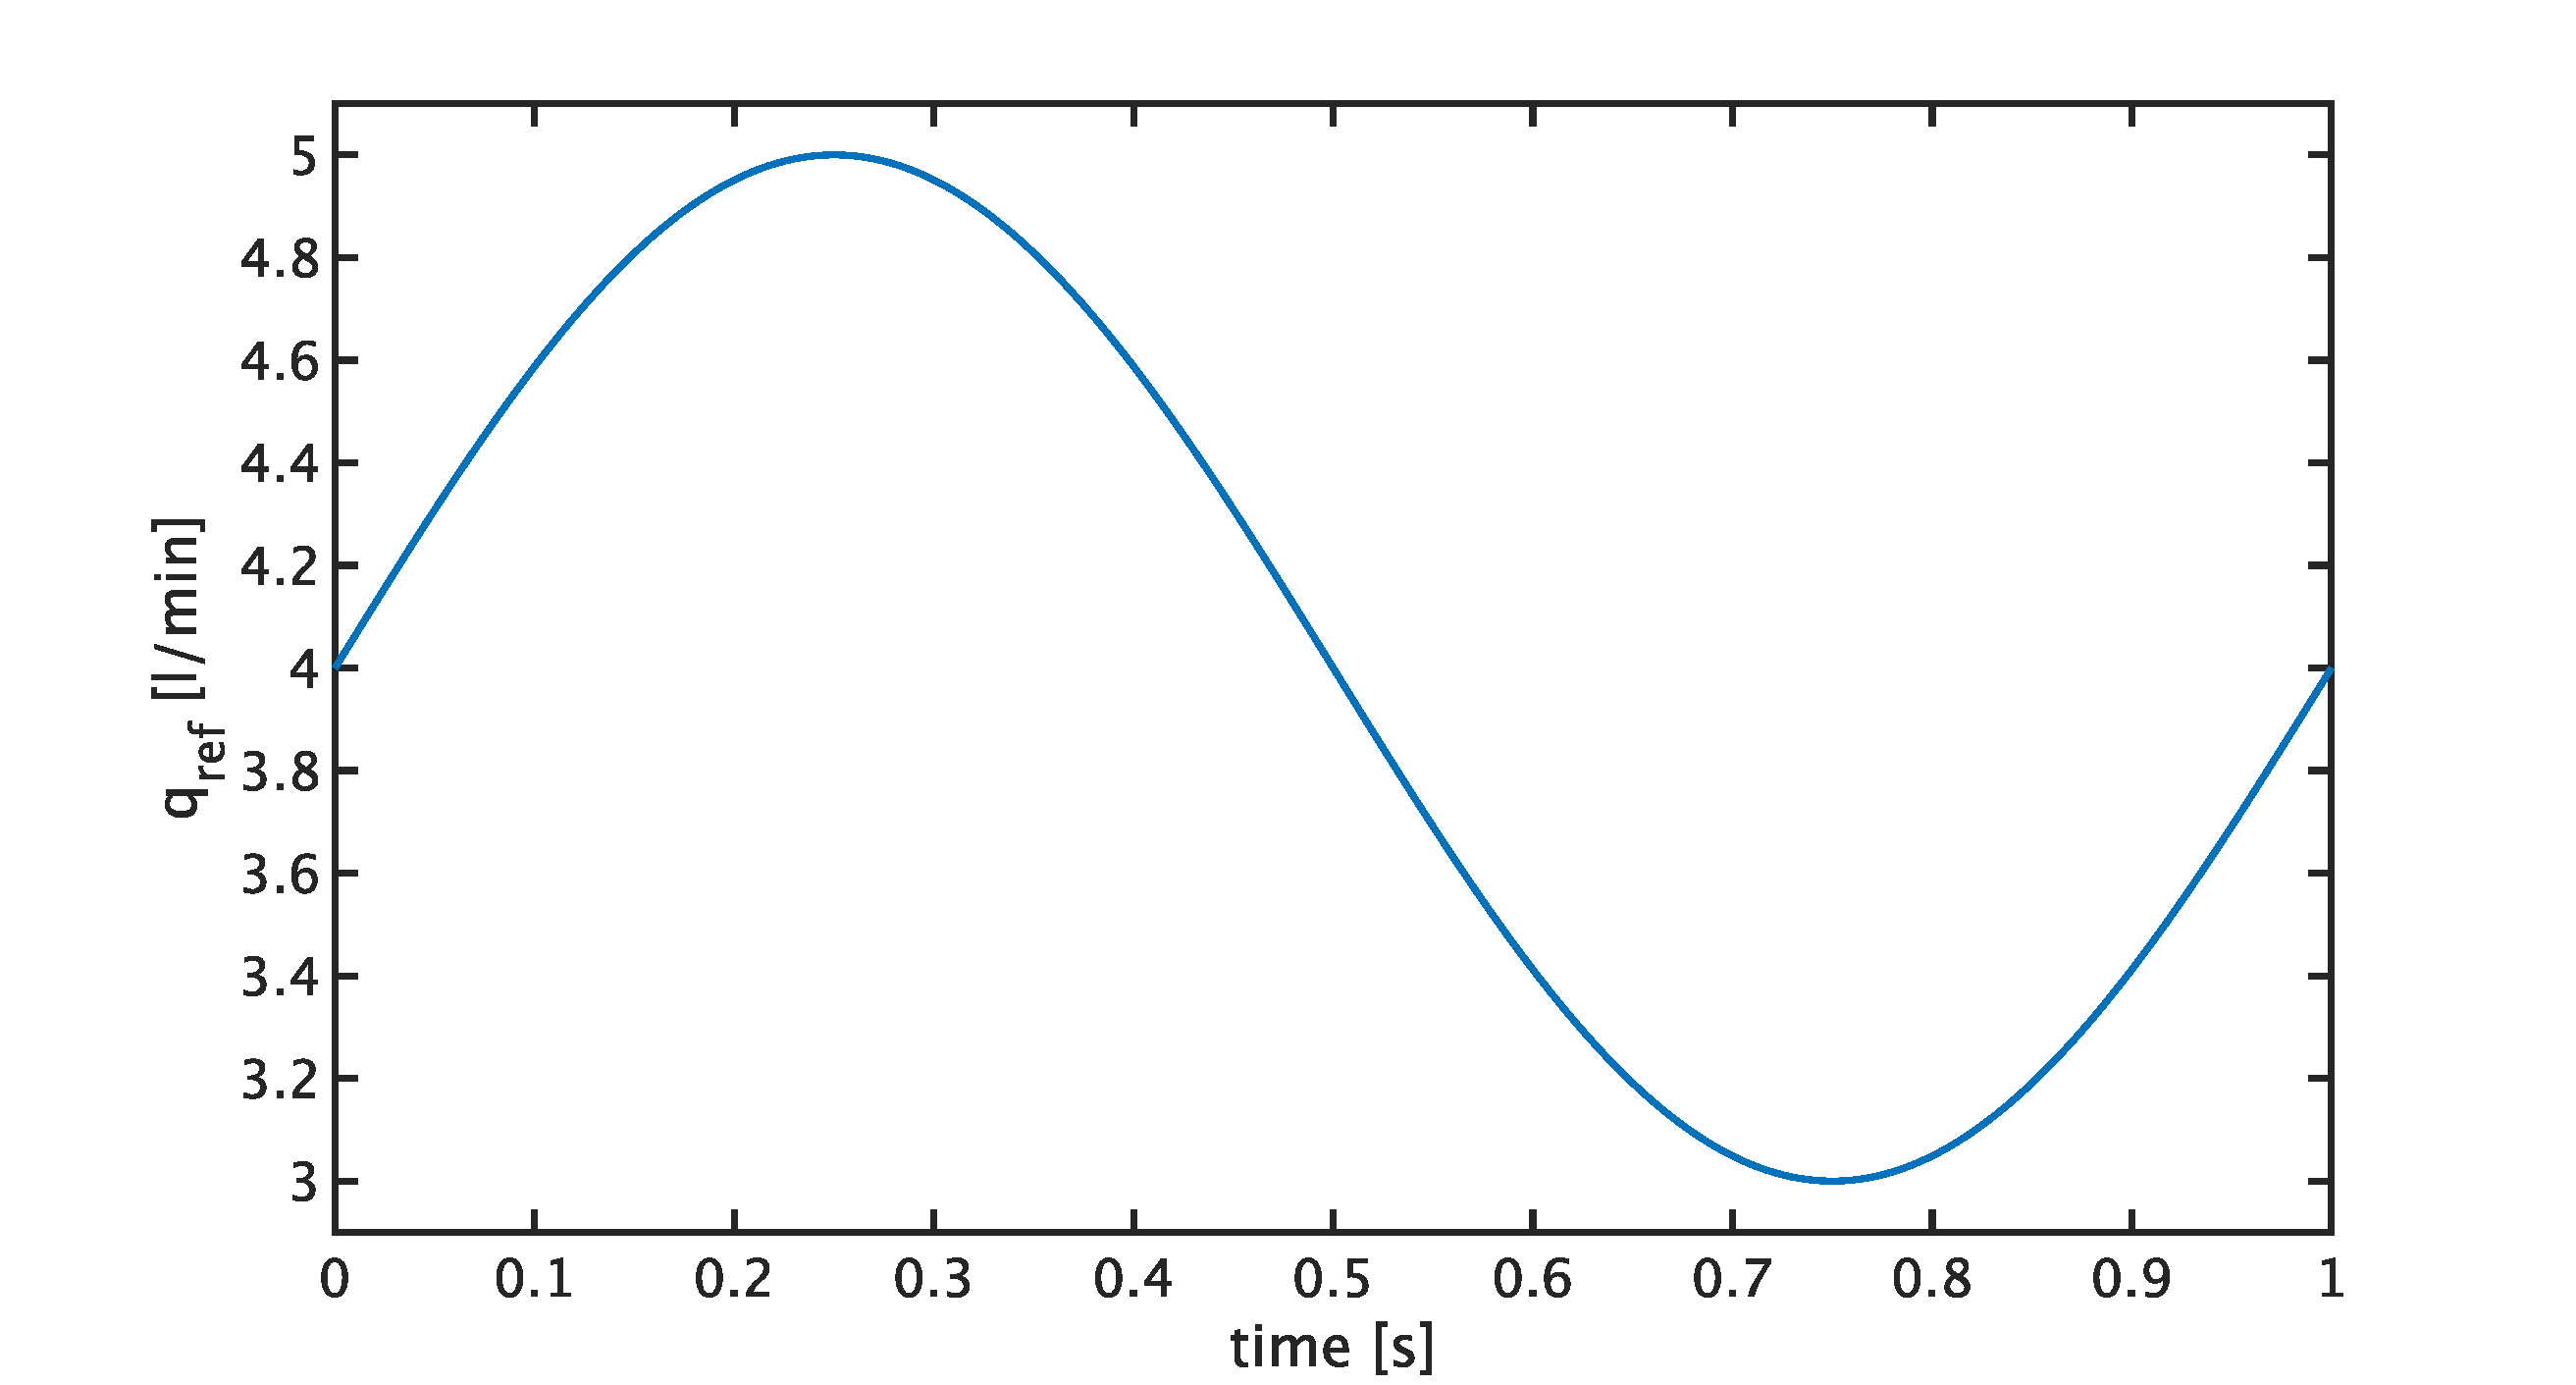
\includegraphics[width=0.5\textwidth]{images/chapt_5/ILC/ref_sine.pdf}\label{fig:ref_sine}}
%   \subfloat[]
%   {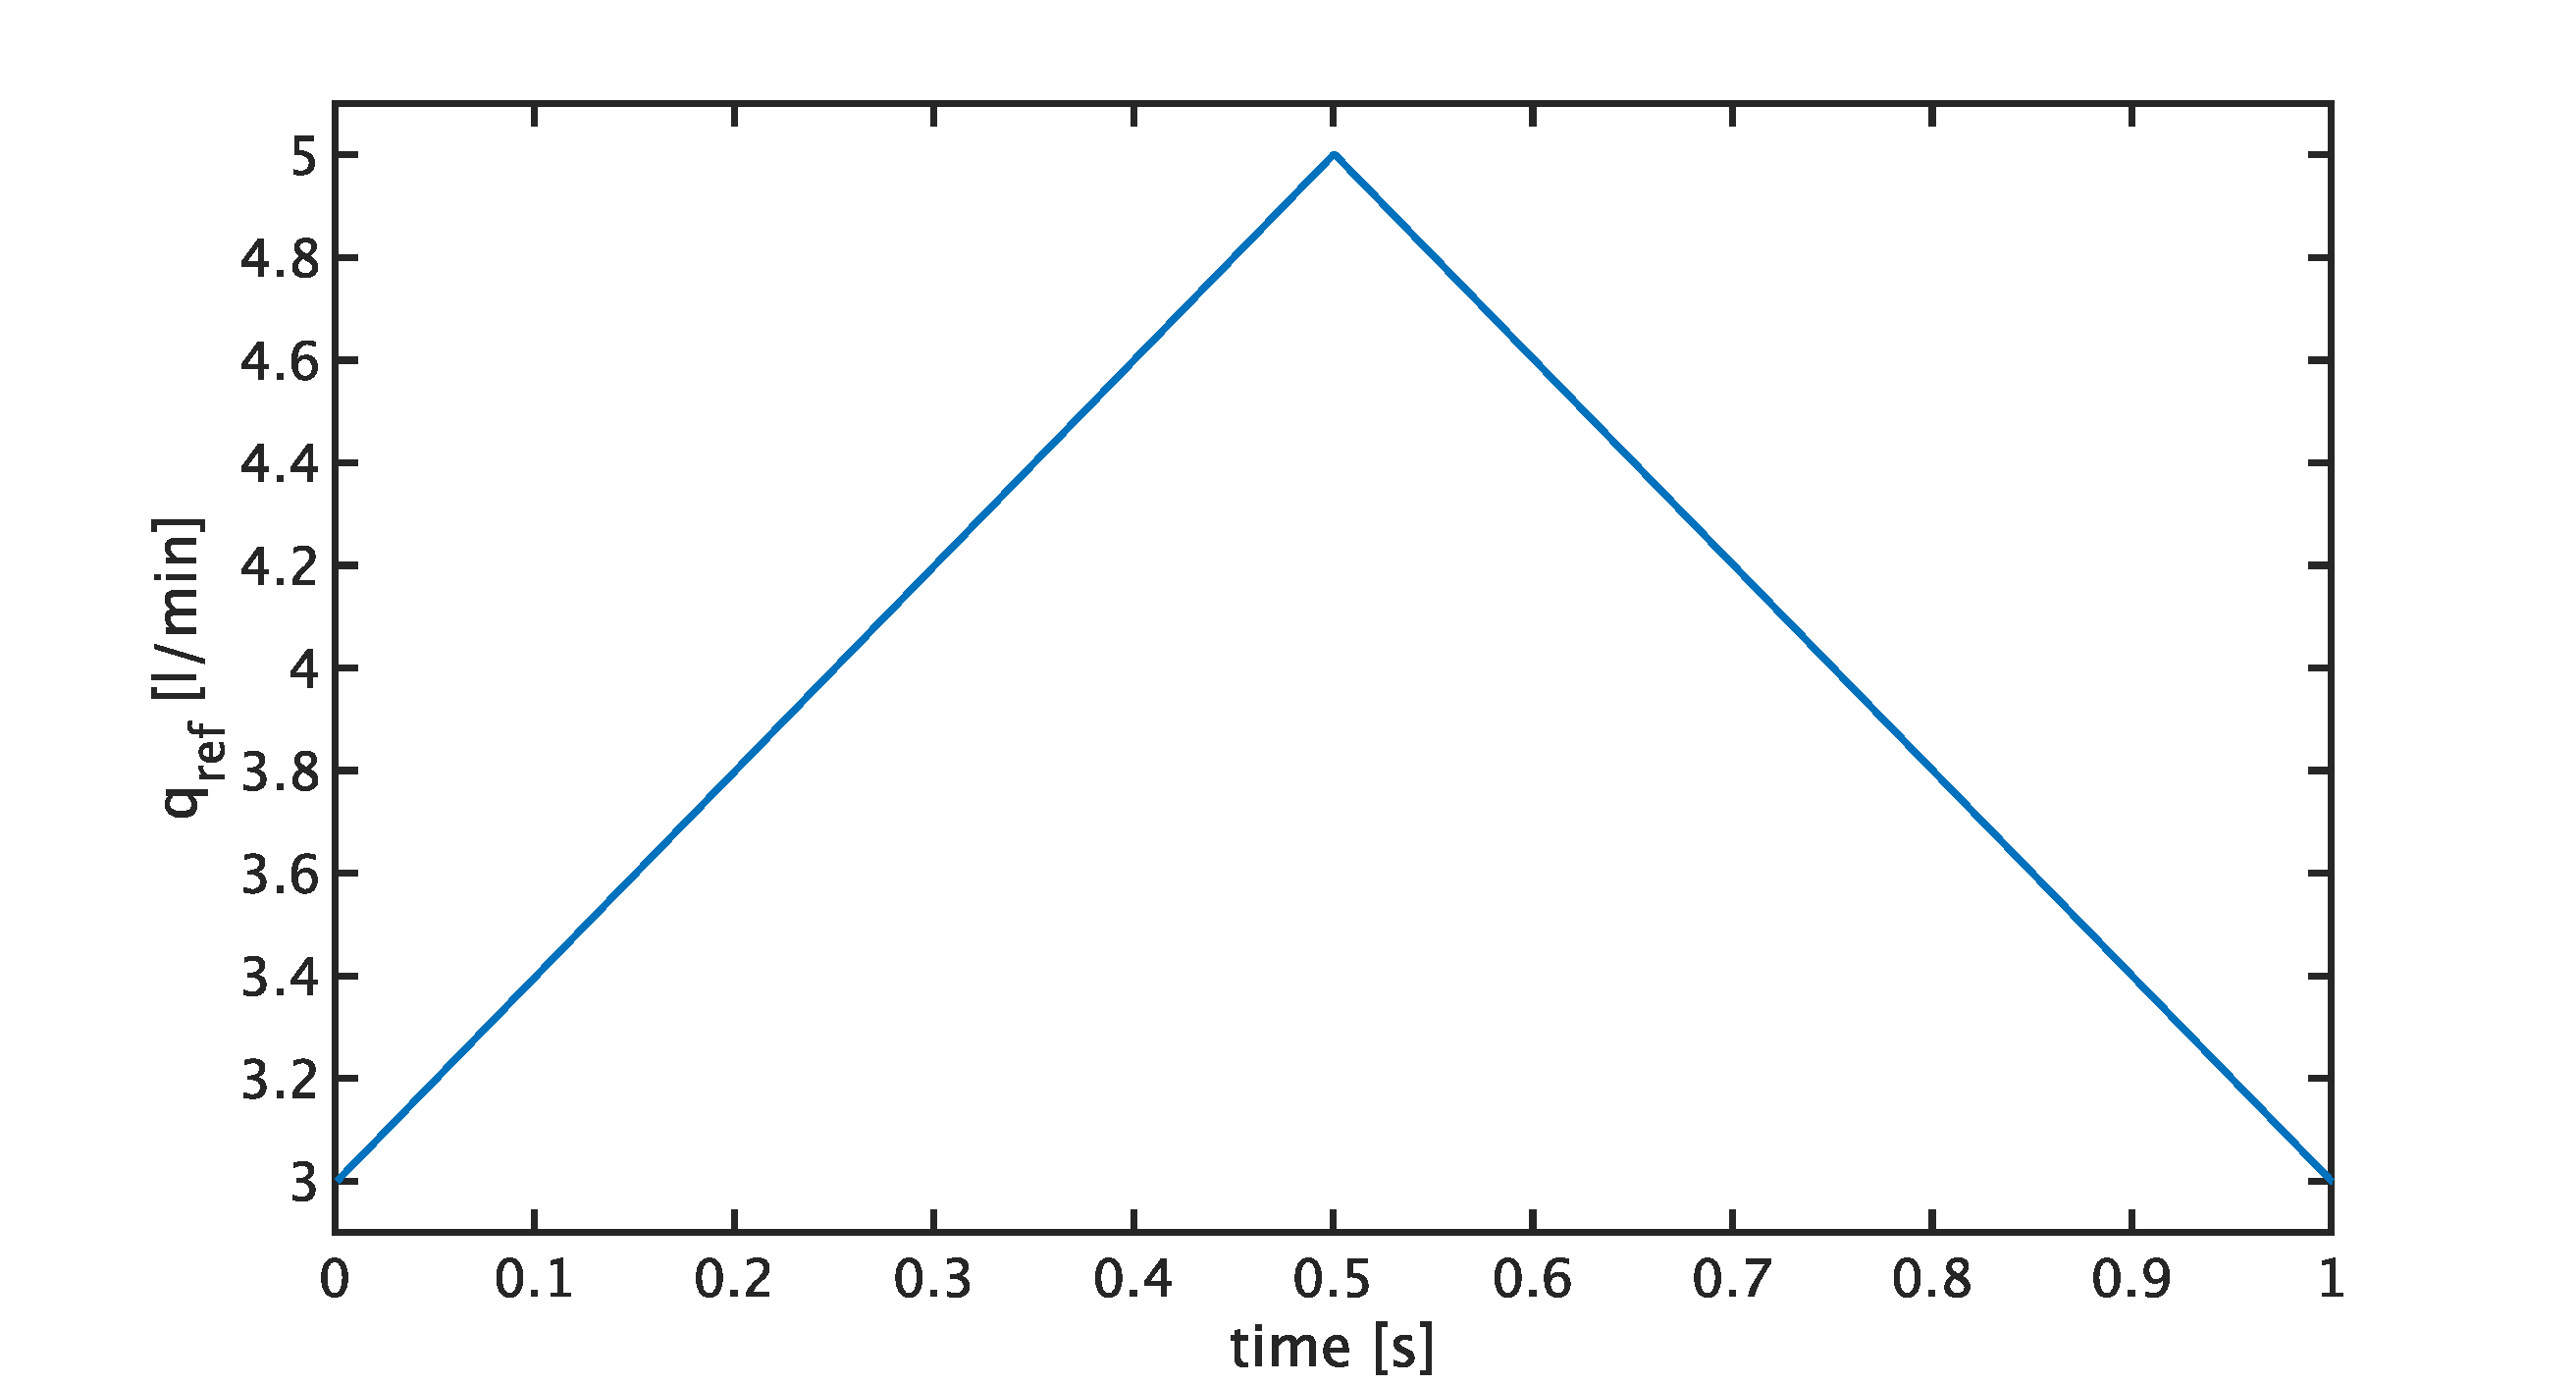
\includegraphics[width=0.5\textwidth]{images/chapt_5/ILC/ref_triang.pdf}\label{fig:ref_triang}}
%   \caption[Control error for PI Controllers]{Control error for PI controllers tuned according to (a) Ziegler Nichols, (b) Chien Hrones Reswick}
%   \label{fig:ref_signals}
% \end{figure}
The third reference trajectory is given in form of a triangular signal. As for the sinusoidal signal, the maximum value is set to $q_{\mathrm{ref}}=5\,l/min$ and the minimum to $3\, l/min$. Again the full signal length is set to $1\,s$ to match a $60\,bpm$ heart rate. \figurename~\ref{fig:ref_triang} depicts one iterations of the reference trajectory.
\begin{figure}[ht]
  \centering
  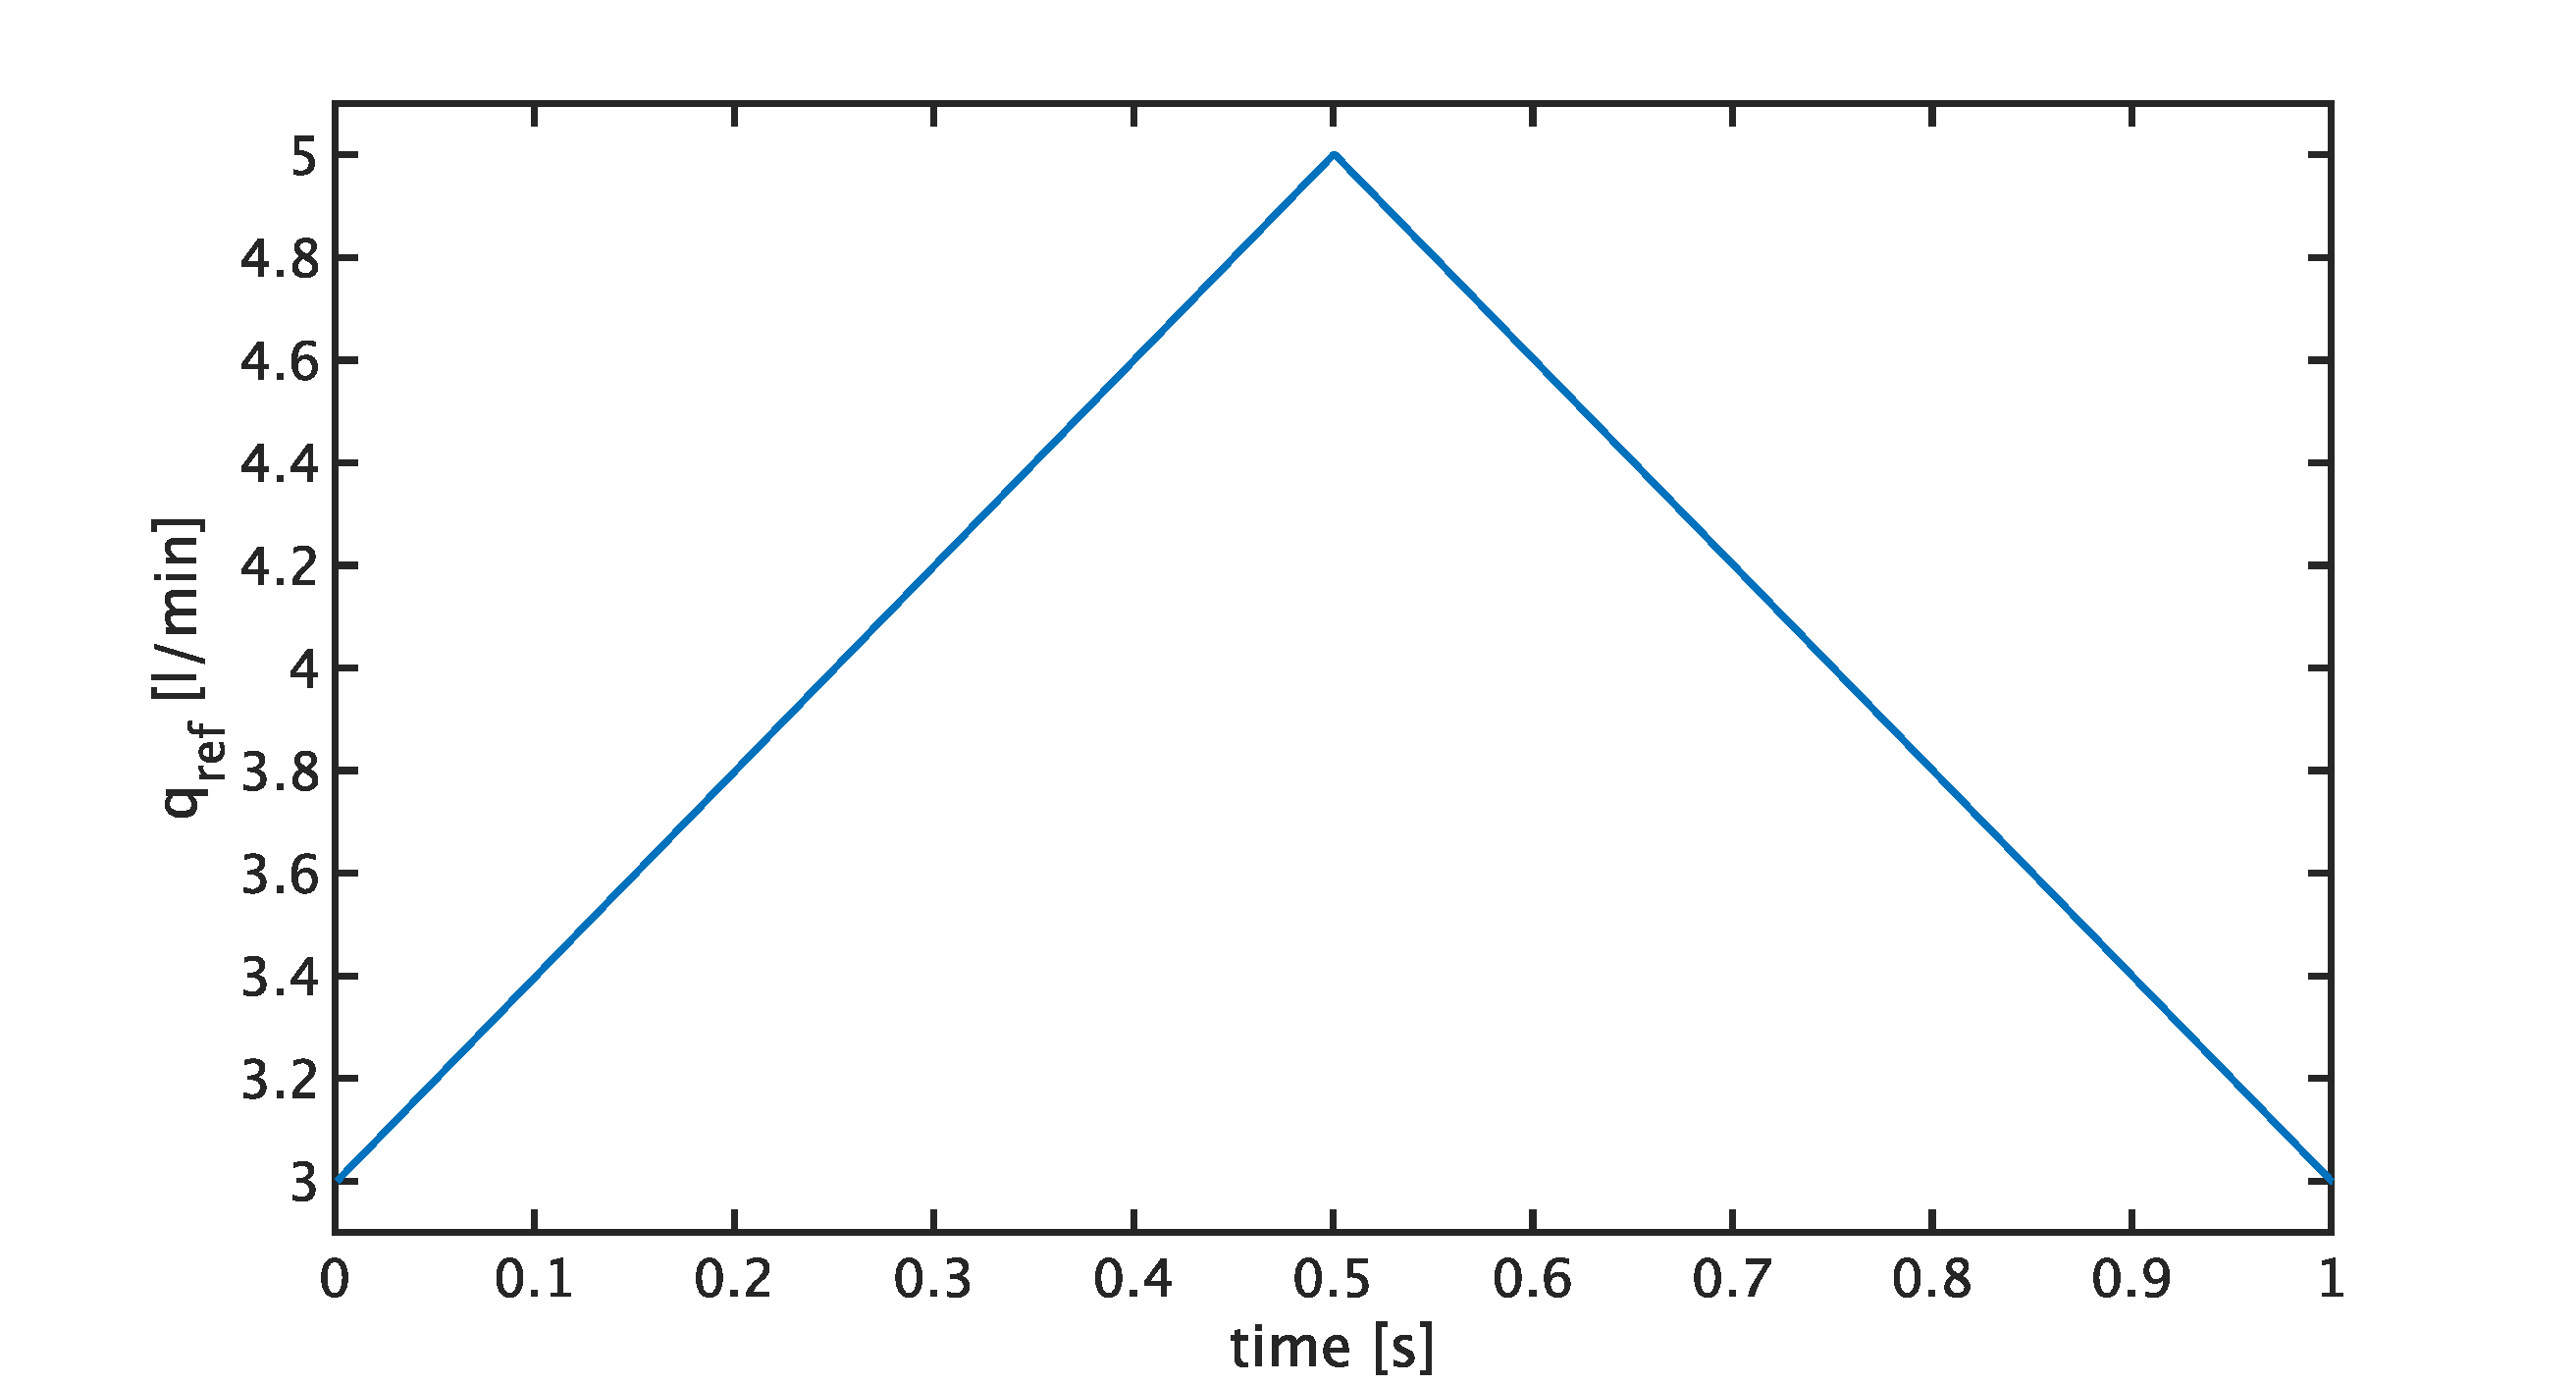
\includegraphics[width=0.95\textwidth]{images/chapt_5/ILC/ref_triang.pdf}
  \caption[Triangular reference signal]{Triangular reference signal.}
  \label{fig:ref_triang}
\end{figure}
\\As a last trajectory a rectangular signal similar to the one used in chapter \ref{ILC_1} is chosen. The upper step is set to $q_{\mathrm{ref}}=5\,l/min$ and the lower one to $q_{\mathrm{ref}}=3\,l/min$. Both are hold for $0.5\,s$. Again the signal is filtered using a $1^{st}$ order butterworth filter with cut off frequency $f_{\mathrm{c}}=20\,Hz$ and sampling frequency $f_{\mathrm{s}}=1000\,Hz$.
\\\figurename~\ref{fig:ref_square} depicts one iteration of the reference.
\begin{figure}[ht]
  \centering
  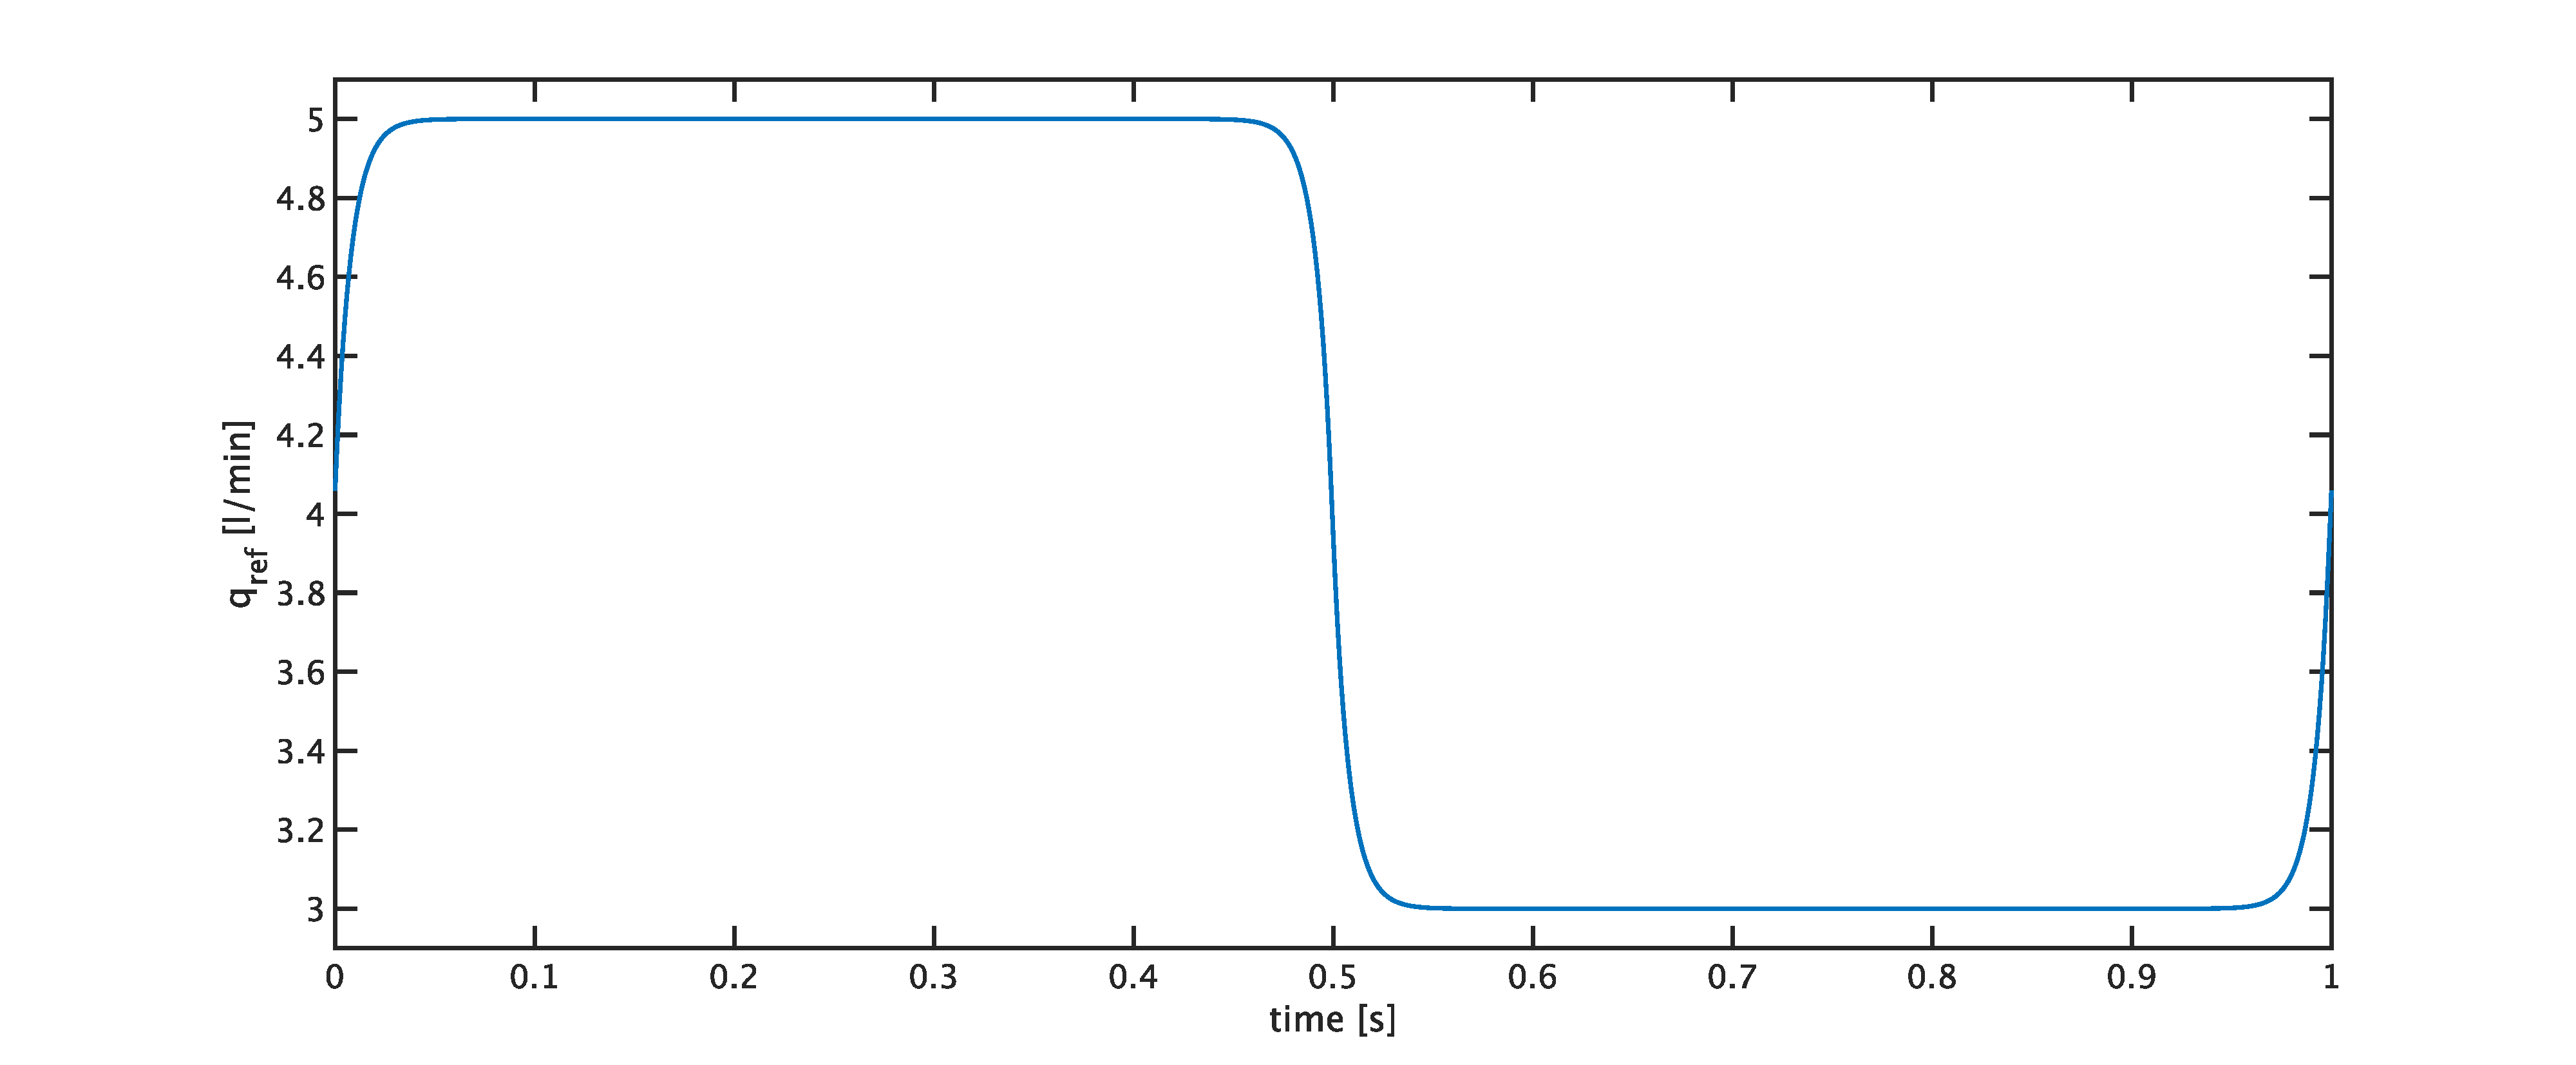
\includegraphics[width=\textwidth]{images/chapt_5/ILC/ref_square.pdf}
  \caption[Rectangular reference signal]{Rectangular reference signal.}
  \label{fig:ref_square}
\end{figure}
%


\subsection{Evaluation}
Using the reference trajectories described above, several measurements are performed and evaluated to determine performance of the ILC subjected to repeating disturbances. Measurements are performed for varying levels of contractility of the left ventricle for all reference trajectories. The performance results of the contractility levels are compared to each other. Contractility is decreased in steps of $0.25$ from $cf_{\mathrm{Lv}}=1$ representing contractility of a healthy heart to $cf_{\mathrm{LV}}=0.25$ correlating to a severe impairment of heart functionality.
\\During all measurements for the first $120\,s$, exclusively PI control is activated to ensure stable system behavior at the beginning of additional ILC control.

In a first step, measurements are performed using the constant reference flow of $q_{\mathrm{ref}}=5\,l/min$. \figurename~\ref{fig:pi_to_ilc_dist_const_cf1} depicts the transition from exclusive PI control \\($115 \-- 120\,s$) to use of the parallel control structure ($120\--130\,s$) for a contractility of $cf_{\mathrm{LV}}=1$. It is evident that the PI controller alone is not able to suppress the disturbance's influence on the flow. As soon as ILC control sets in the flow settles further towards the constant reference flow with each ILC iteration.
\begin{figure}[ht!]
  \centering
  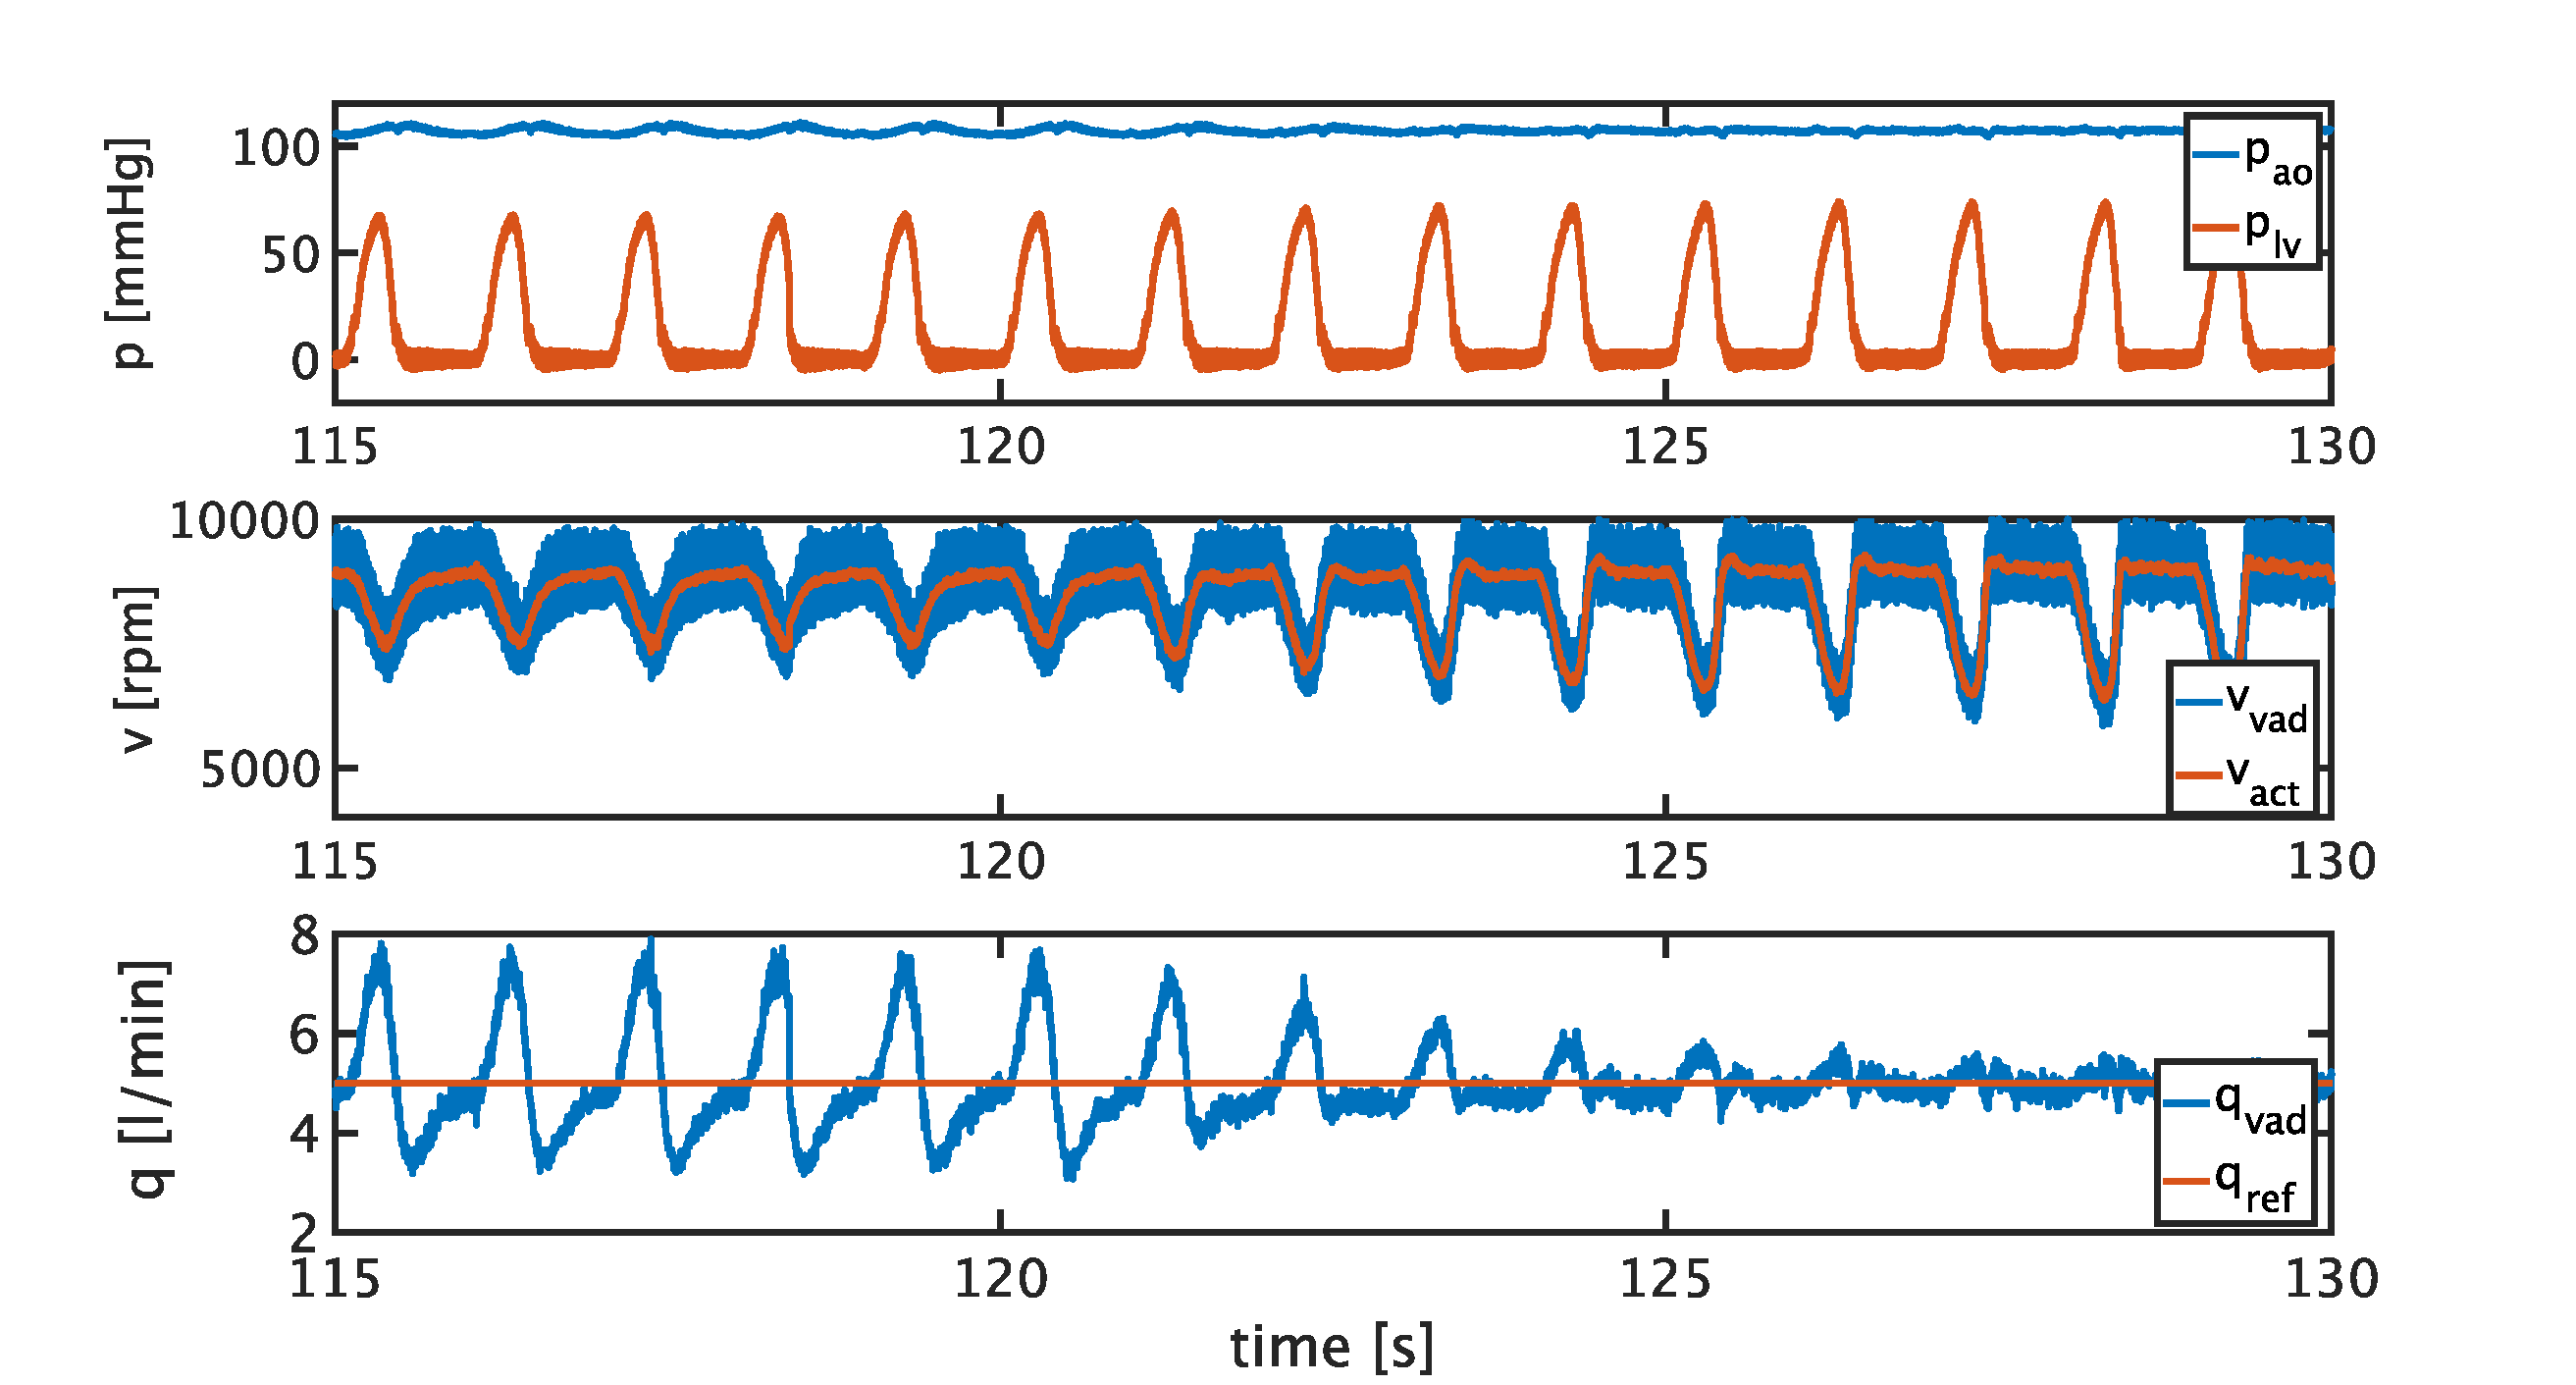
\includegraphics[width=0.95\textwidth]{images/chapt_5/ILC/pi_to_ilc_dist_const_cf1.pdf}
  \caption[Segment of measurement for ILC with disturbance of $HR=60\,bpm$ with $cf_{\mathrm{Lv}}=1$ for constant reference flow]{Segment of measurement for ILC with disturbance of $HR=60\,bpm$ with $cf_{\mathrm{Lv}}=1$ for constant reference flow. Top:  pressure values of the MCL. Middle: actuating variable and measured rotational speed of the VAD. Bottom: targeted flow trajectory and measured flow through the VAD.}
  \label{fig:pi_to_ilc_dist_const_cf1}
\end{figure}
\\Measurements for all contractility levels are running stable until the end of measurement time is reached at $600\,s$. A comparison of the RMSE values for each iteration is presented in \figurename~\ref{fig:RMSE_dist_const_5_var_cf}.
\begin{figure}[ht]
  \centering
  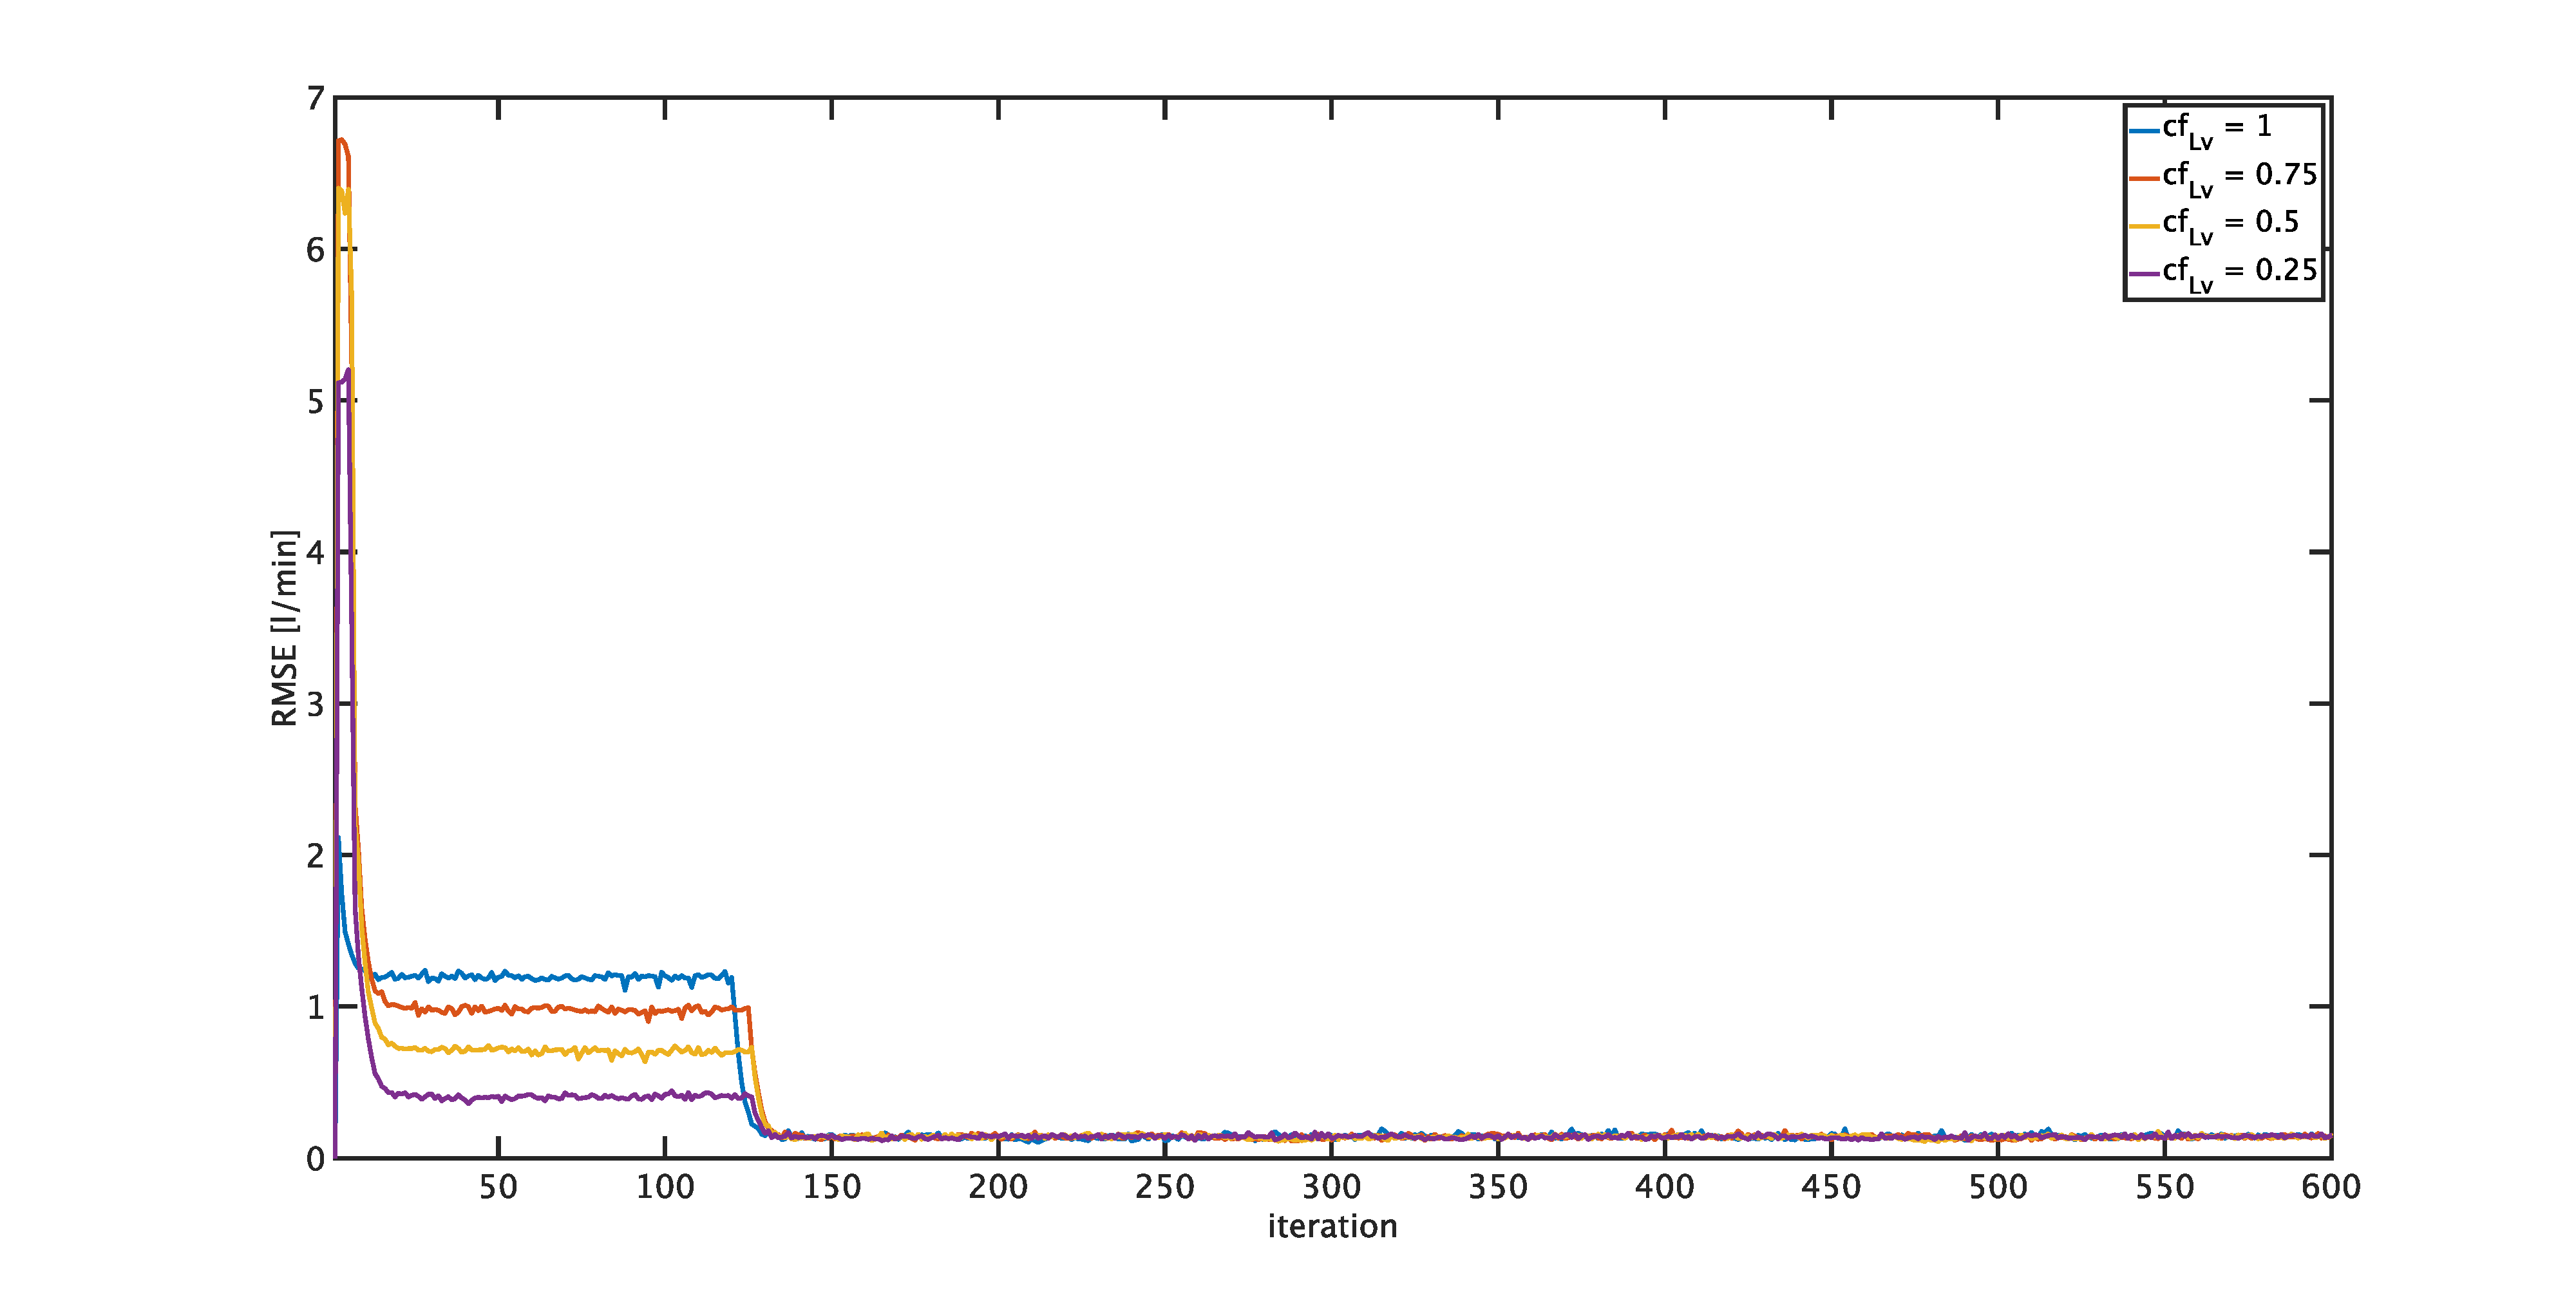
\includegraphics[width=0.9\textwidth]{images/chapt_5/ILC/RMSE_dist_const_5_var_cf.pdf}
  \caption[RMSE Comparison of ILC at constant reference flow for varying left ventricular contractilities]{Comparison of RMSE values of the ILC for constant reference flow with disturbance of $HR=60\,bpm$ for varying contractility values of the left ventricle.}
  \label{fig:RMSE_dist_const_5_var_cf}
\end{figure}


Up to iteration 120, the graph represents the RMSE of the PI controller. For this time, it is evident that with decreasing left ventricular contractility RMSE also decreases from $RMSE_{\mathrm{PI,const,cf_{Lv}=1}}\approx 1.2\, l/min$ to $RMSE_{\mathrm{PI,const,cf_{Lv}=0.25}}\approx 0.4\, l/min$. This can be explained with the lower influence of pressure changes due to weakened contractility. The RMSE values for all four contractility levels using combined PI and ILC control amount to
\begin{equation}
  RMSE_{\mathrm{ILC,const}}\approx0.14\,l/min.
\end{equation}
It is evident that using the combined control approach results in significantly higher performance in all contractility ranges for a constant reference flow.

The next measurements performed are the ones testing the controller's ability to follow the sinusoidal reference trajectory. The trajectory is placed synchronous to the heart beat. \figurename~\ref{fig:pi_to_ilc_dist_sine_cf1} illustrates the transition phase from PI to combined control for the sinusoidal reference at $cf_{\mathrm{Lv}}=1$.
\begin{figure}[ht!]
  \centering
  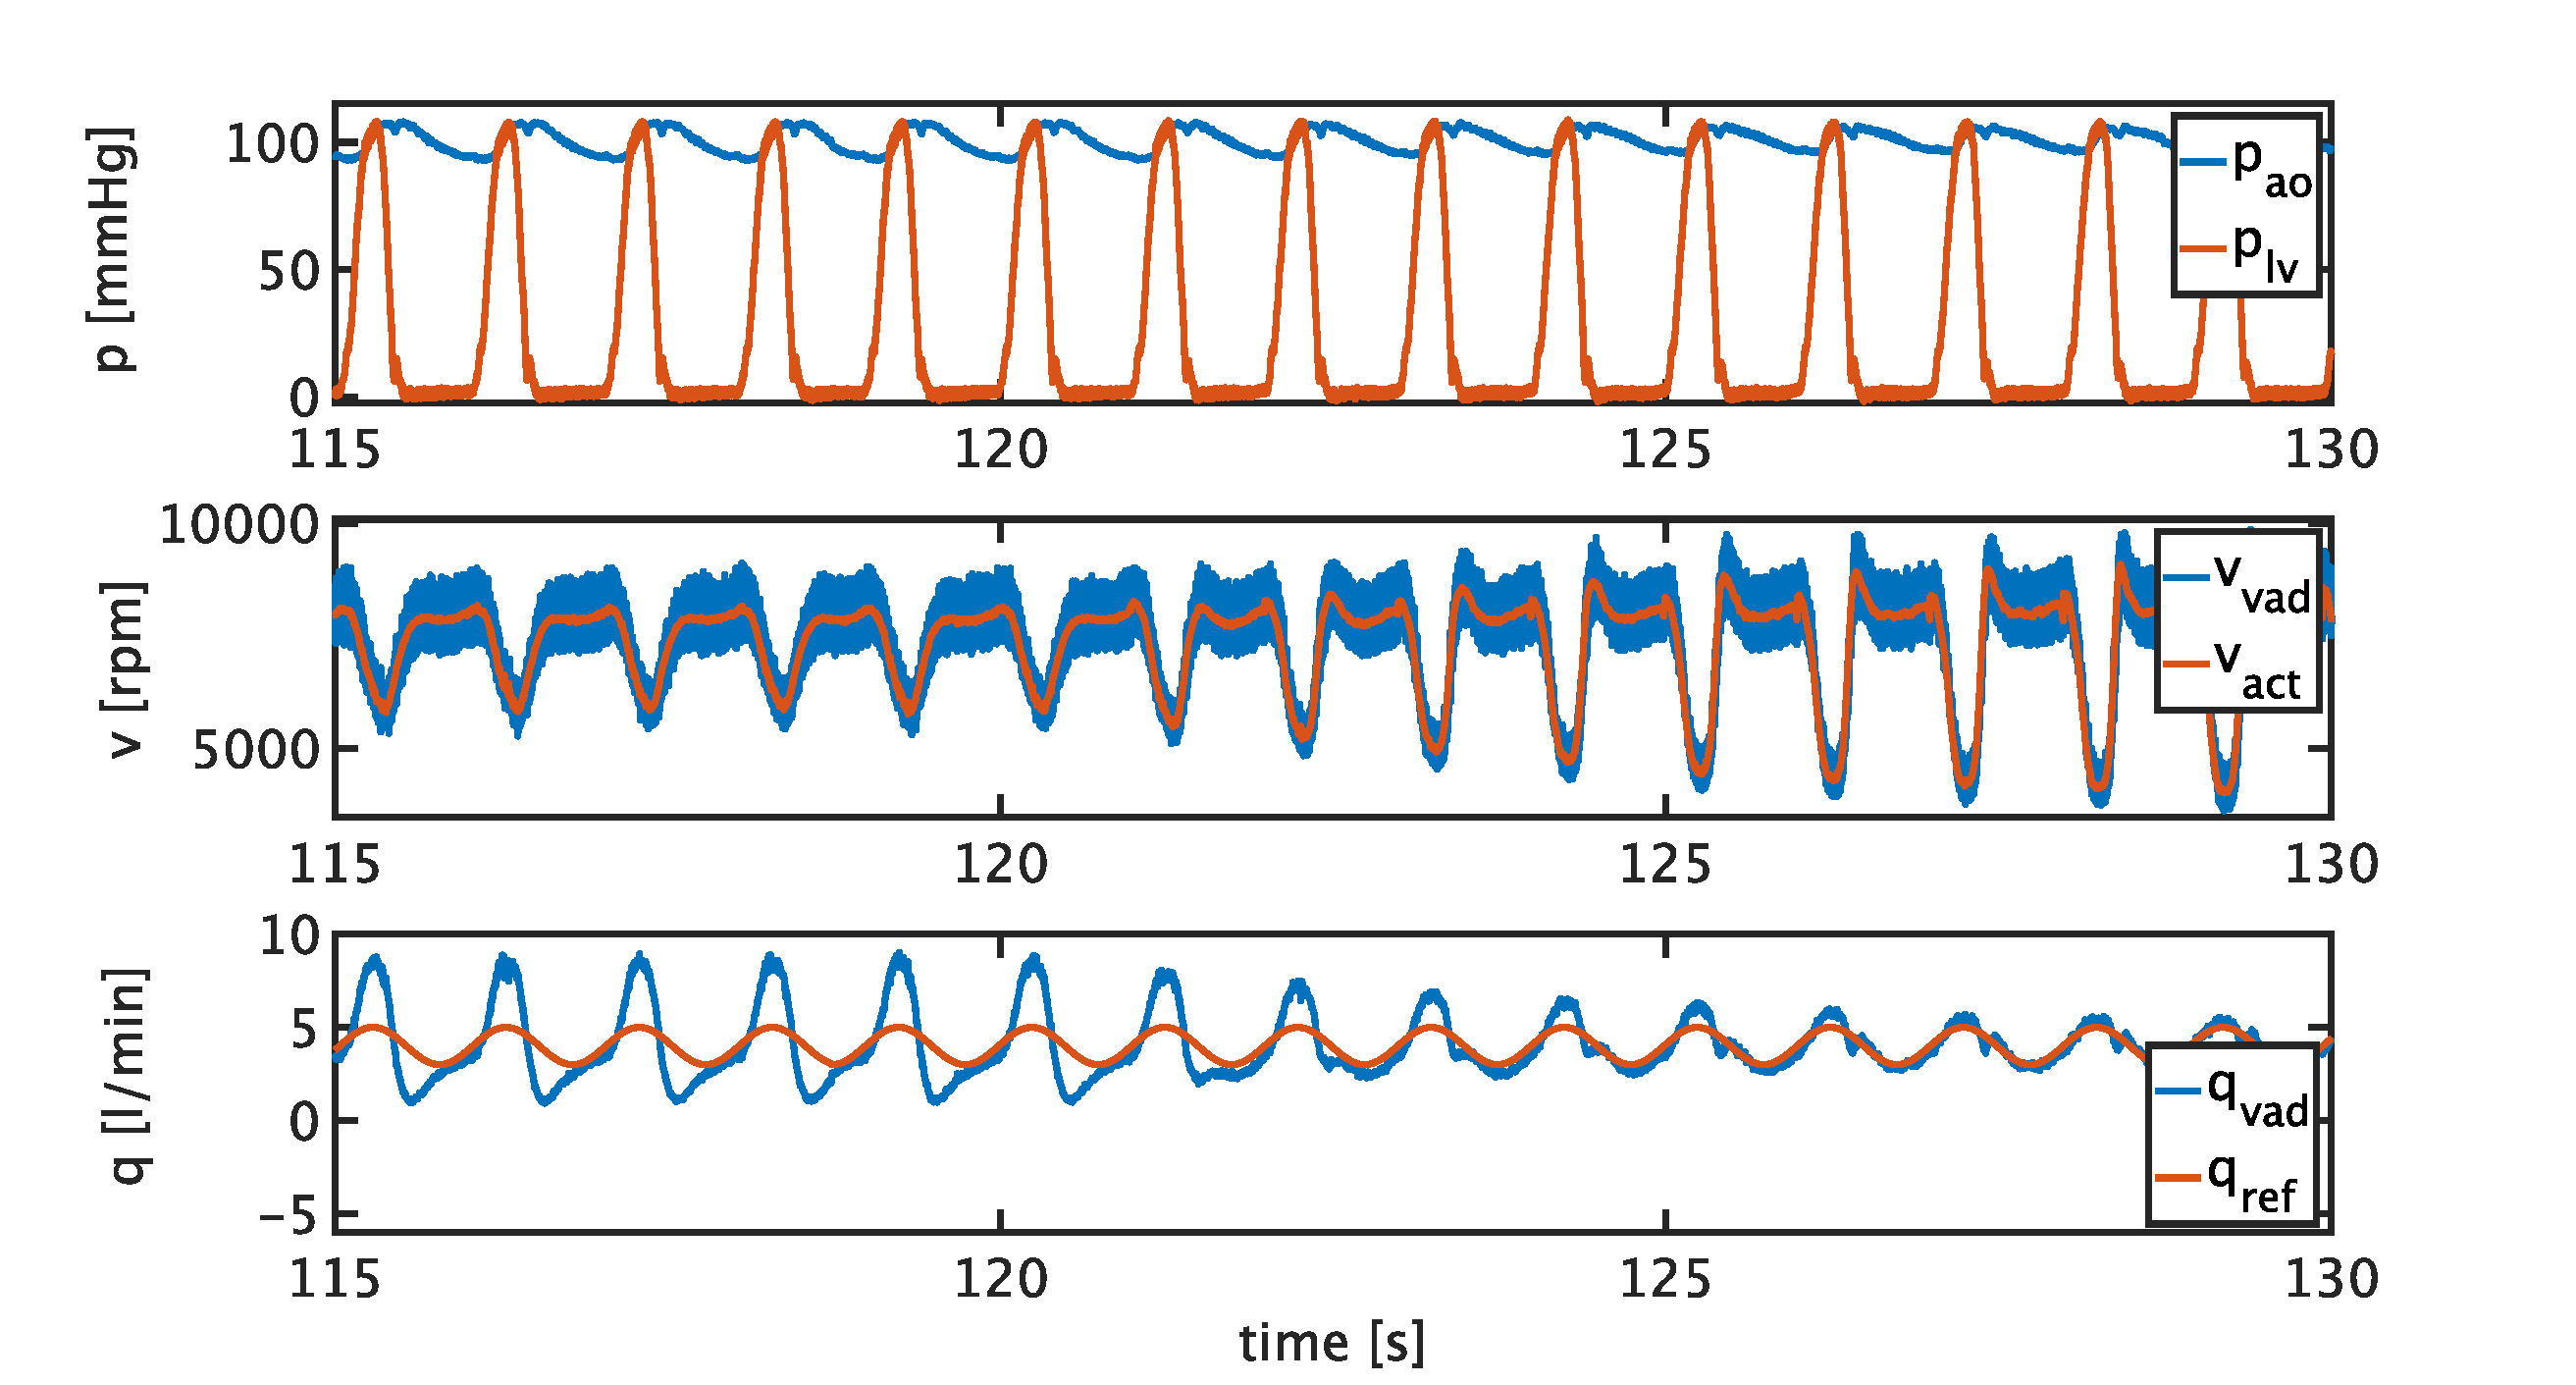
\includegraphics[width=0.95\textwidth]{images/chapt_5/ILC/pi_to_ilc_dist_sine_cf1.pdf}
  \caption[Segment of measurement for ILC with disturbance of $HR=60\,bpm$ with $cf_{\mathrm{Lv}}=1$ for sinusoidal reference flow]{Segment of measurement for ILC with disturbance of $HR=60\,bpm$ with $cf_{\mathrm{Lv}}=1$ for sinusoidal reference flow. Top:  pressure values of the MCL. Middle: actuating variable and measured rotational speed of the VAD. Bottom: targeted flow trajectory and measured flow through the VAD}
  \label{fig:pi_to_ilc_dist_sine_cf1}
\end{figure}
Similar to the constant reference flow, the PI controller alone is not able to follow the reference trajectory. The combination between PI controller and ILC, however, leads to a clearly recognizable improvement of the following behavior within some iterations.
The comparison of RMSE values (see \figurename~\ref{fig:RMSE_dist_sine_var_cf}) leads to similar conclusions as for the constant reference flow. During the first 120 iterations when only PI control is active RMSE decreases with decreasing contractility of the left ventricle. However, the decrease between contractility values from $cf_{\mathrm{LV}}=1$ to $cf_{\mathrm{LV}}=0.75$ and $cf_{\mathrm{LV}}=0.5$ with $RMSE_{\mathrm{PI,sine,cf_{\mathrm{Lv}}=1}}\approx 1.85\, l/min$, $RMSE_{\mathrm{PI,sine,cf_{\mathrm{Lv}}=0.75}}\approx 1.75\, l/min$ and $RMSE_{\mathrm{PI,sine,cf_{\mathrm{Lv}}=1}}\approx 1.85\, l/min$, are less significant than the reduction of contractility to $cf_{\mathrm{Lv}}=0.25$ with $RMSE_{\mathrm{PI,sine,cf_{\mathrm{Lv}}=0.25}}\approx 0.93\, l/min$.
\begin{figure}[ht!]
  \centering
  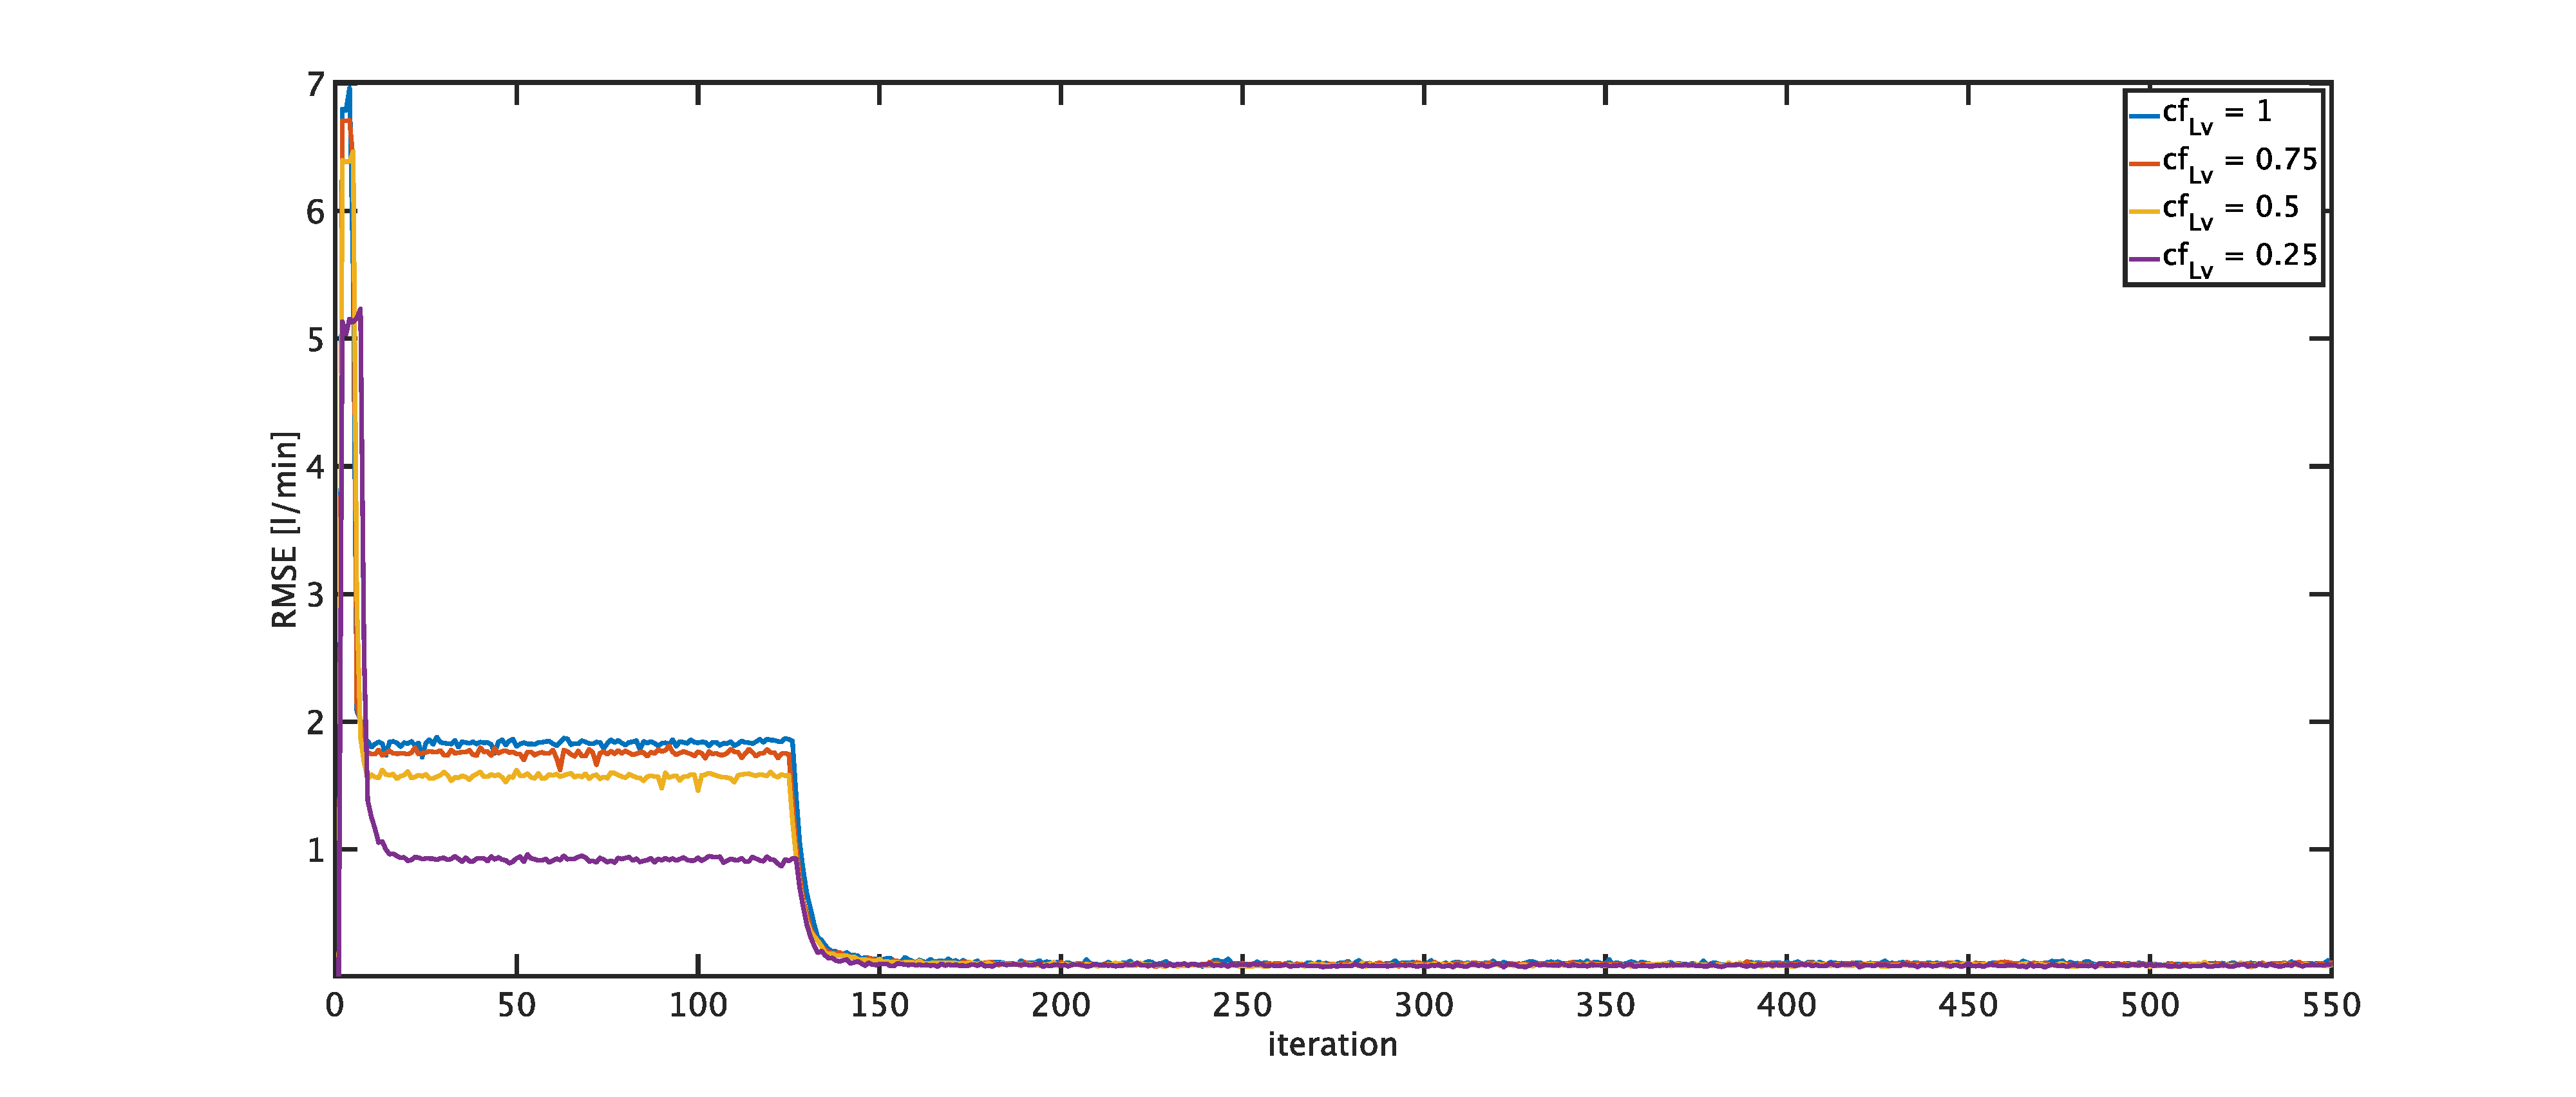
\includegraphics[width=0.9\textwidth]{images/chapt_5/ILC/RMSE_dist_sine_var_cf.pdf}
  \caption[RMSE Comparison of ILC at sinusoidal reference flow for varying left ventricular contractilities]{Comparison of RMSE values of the ILC for sinusoidal reference flow with disturbance of $HR=60\,bpm$ for varying contractility values of the left ventricle.}
  \label{fig:RMSE_dist_sine_var_cf}
\end{figure}
Performance for the combined control approach is almost equal for all contractility values with
\begin{equation}
  RMSE_{\mathrm{ILC,sine}}\approx 0.09\, l/min
\end{equation}
and RMSE indicates an increased performance in all cases.

Measurement for the triangular reference trajectory shows slowly oscillating behavior for left ventricular contractility at $cf_{\mathrm{Lv}}=1$ and $cf_{\mathrm{Lv}}=0.75$. \figurename~\ref{fig:pi_to_ilc_dist_triang_cf1}, representing the measurement at $cf_{\mathrm{Lv}}=1$, shows that from the onset of the ILC, initially, a clear approximation to the reference signal is achieved, but the actuating variable $v_{\mathrm{act}}$ (middle graph) continues to reach its saturation limits with each iteration. This ultimately leads to a stoppage of the pump.
\begin{figure}[ht!]
  \centering
  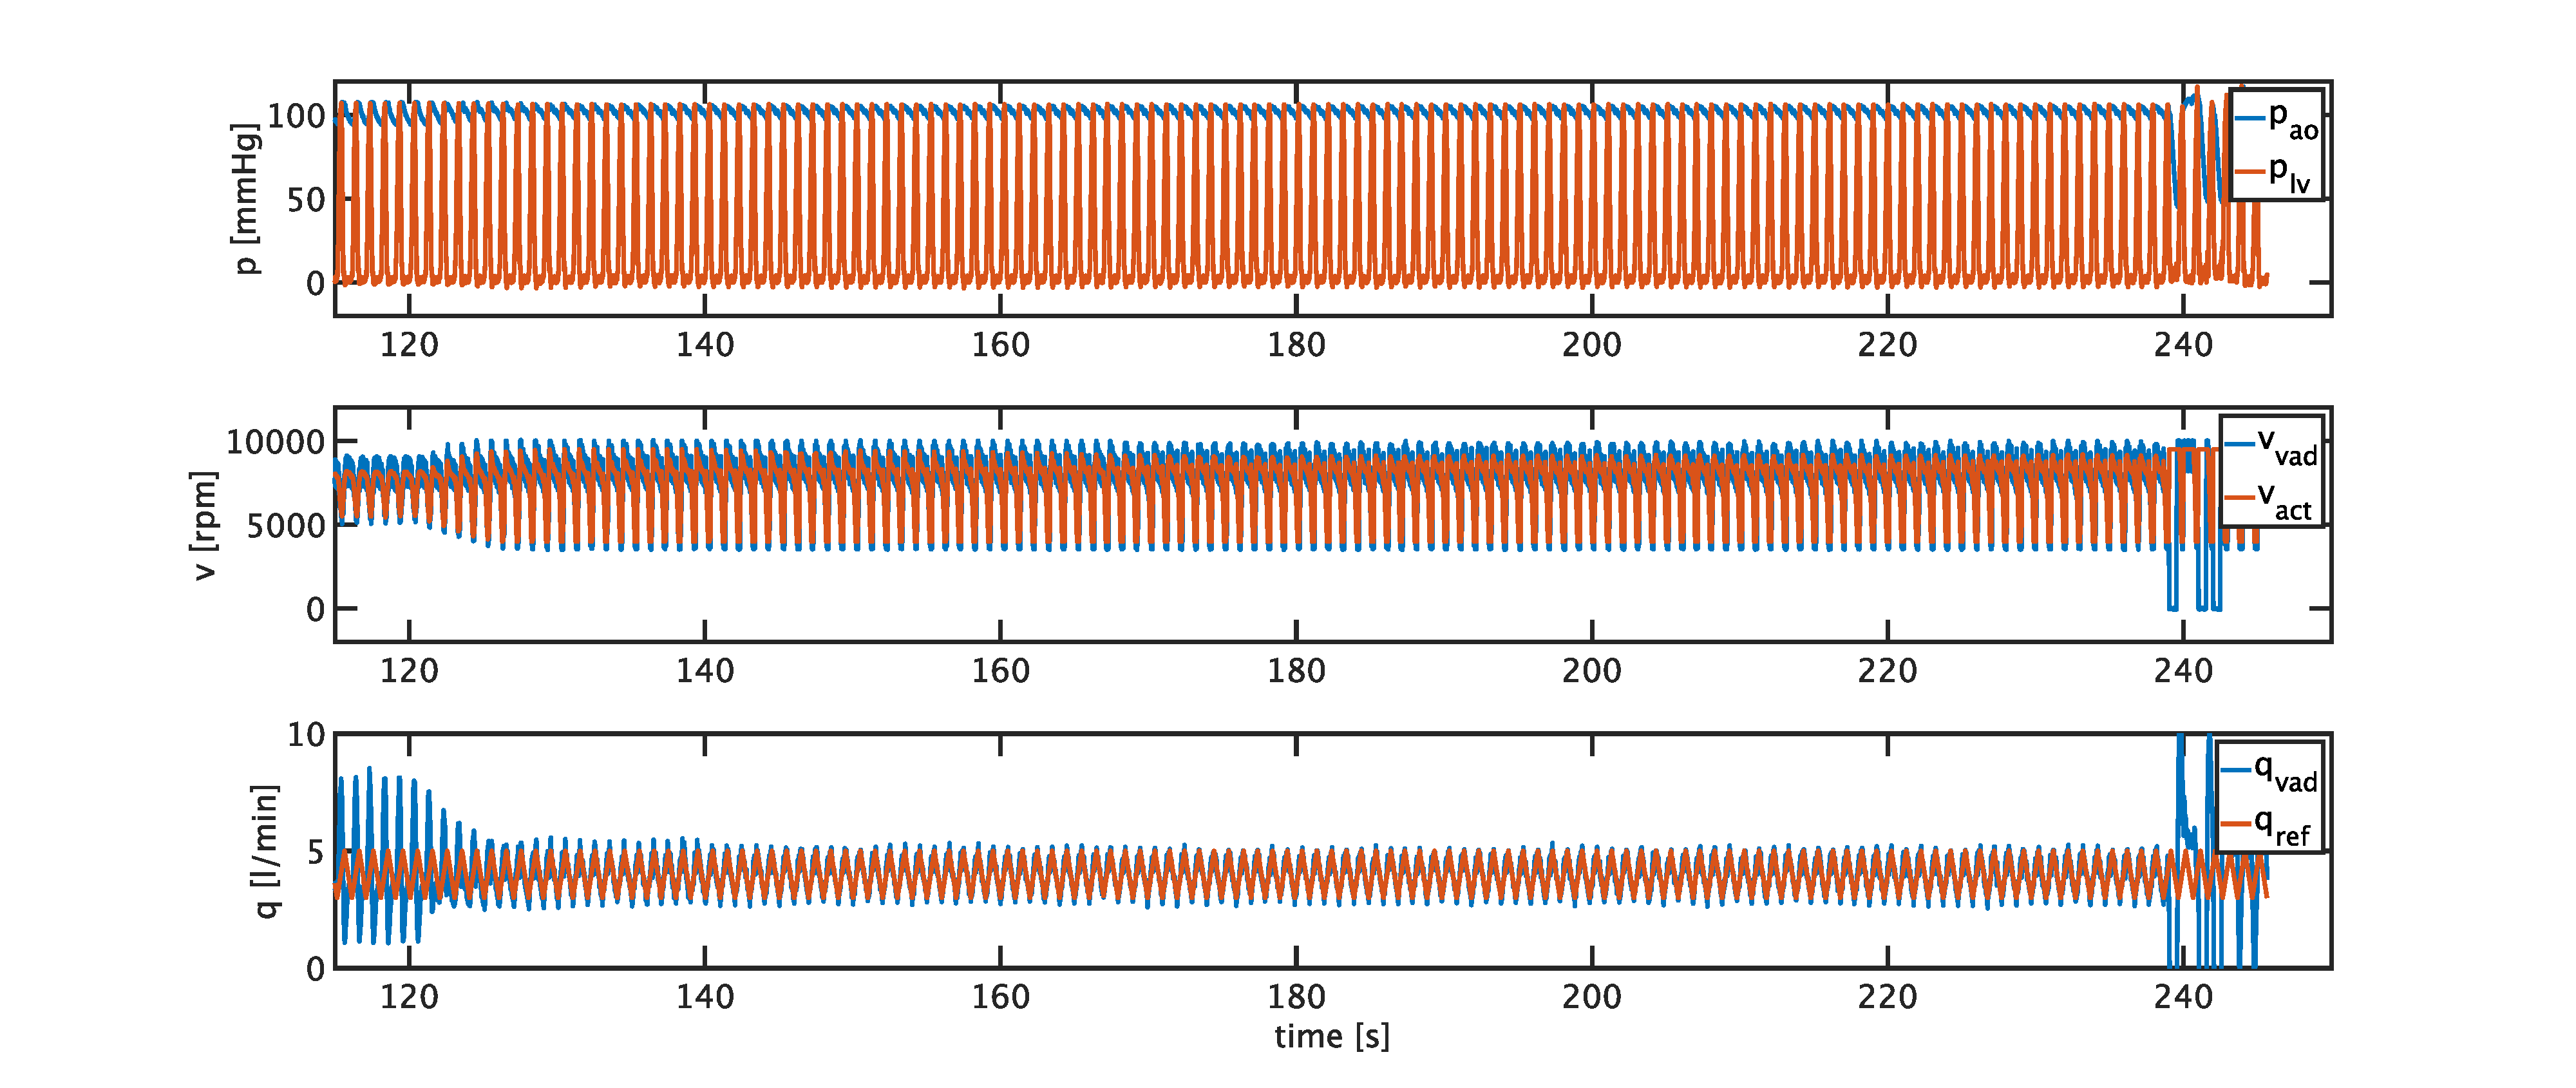
\includegraphics[width=0.95\textwidth]{images/chapt_5/ILC/pi_to_ilc_dist_triang_cf1.pdf}
  \caption[Measurement for ILC with disturbance of $HR=60\,bpm$ with $cf_{\mathrm{Lv}}=1$ for triangular reference flow]{Measurement for ILC with disturbance of $HR=60\,bpm$ with $cf_{\mathrm{Lv}}=1$ for triangular reference flow. Top:  pressure values of the MCL. Middle: actuating variable and measured rotational speed of the VAD. Bottom: targeted flow trajectory and measured flow through the VAD}
  \label{fig:pi_to_ilc_dist_triang_cf1}
\end{figure}
\\Measurements for contractility values $cf_{\mathrm{Lv}}=0.5$ and $cf_{\mathrm{Lv}}=0.25$ show stable behavior over the complete measurement time of $600\,s$. The transition segment for the measurement at $cf_{\mathrm{Lv}}=0.5$ shown in \figurename~\ref{fig:pi_to_ilc_dist_triang_cf50} again indicates an improved performance for the ILC.
\begin{figure}[ht!]
  \centering
  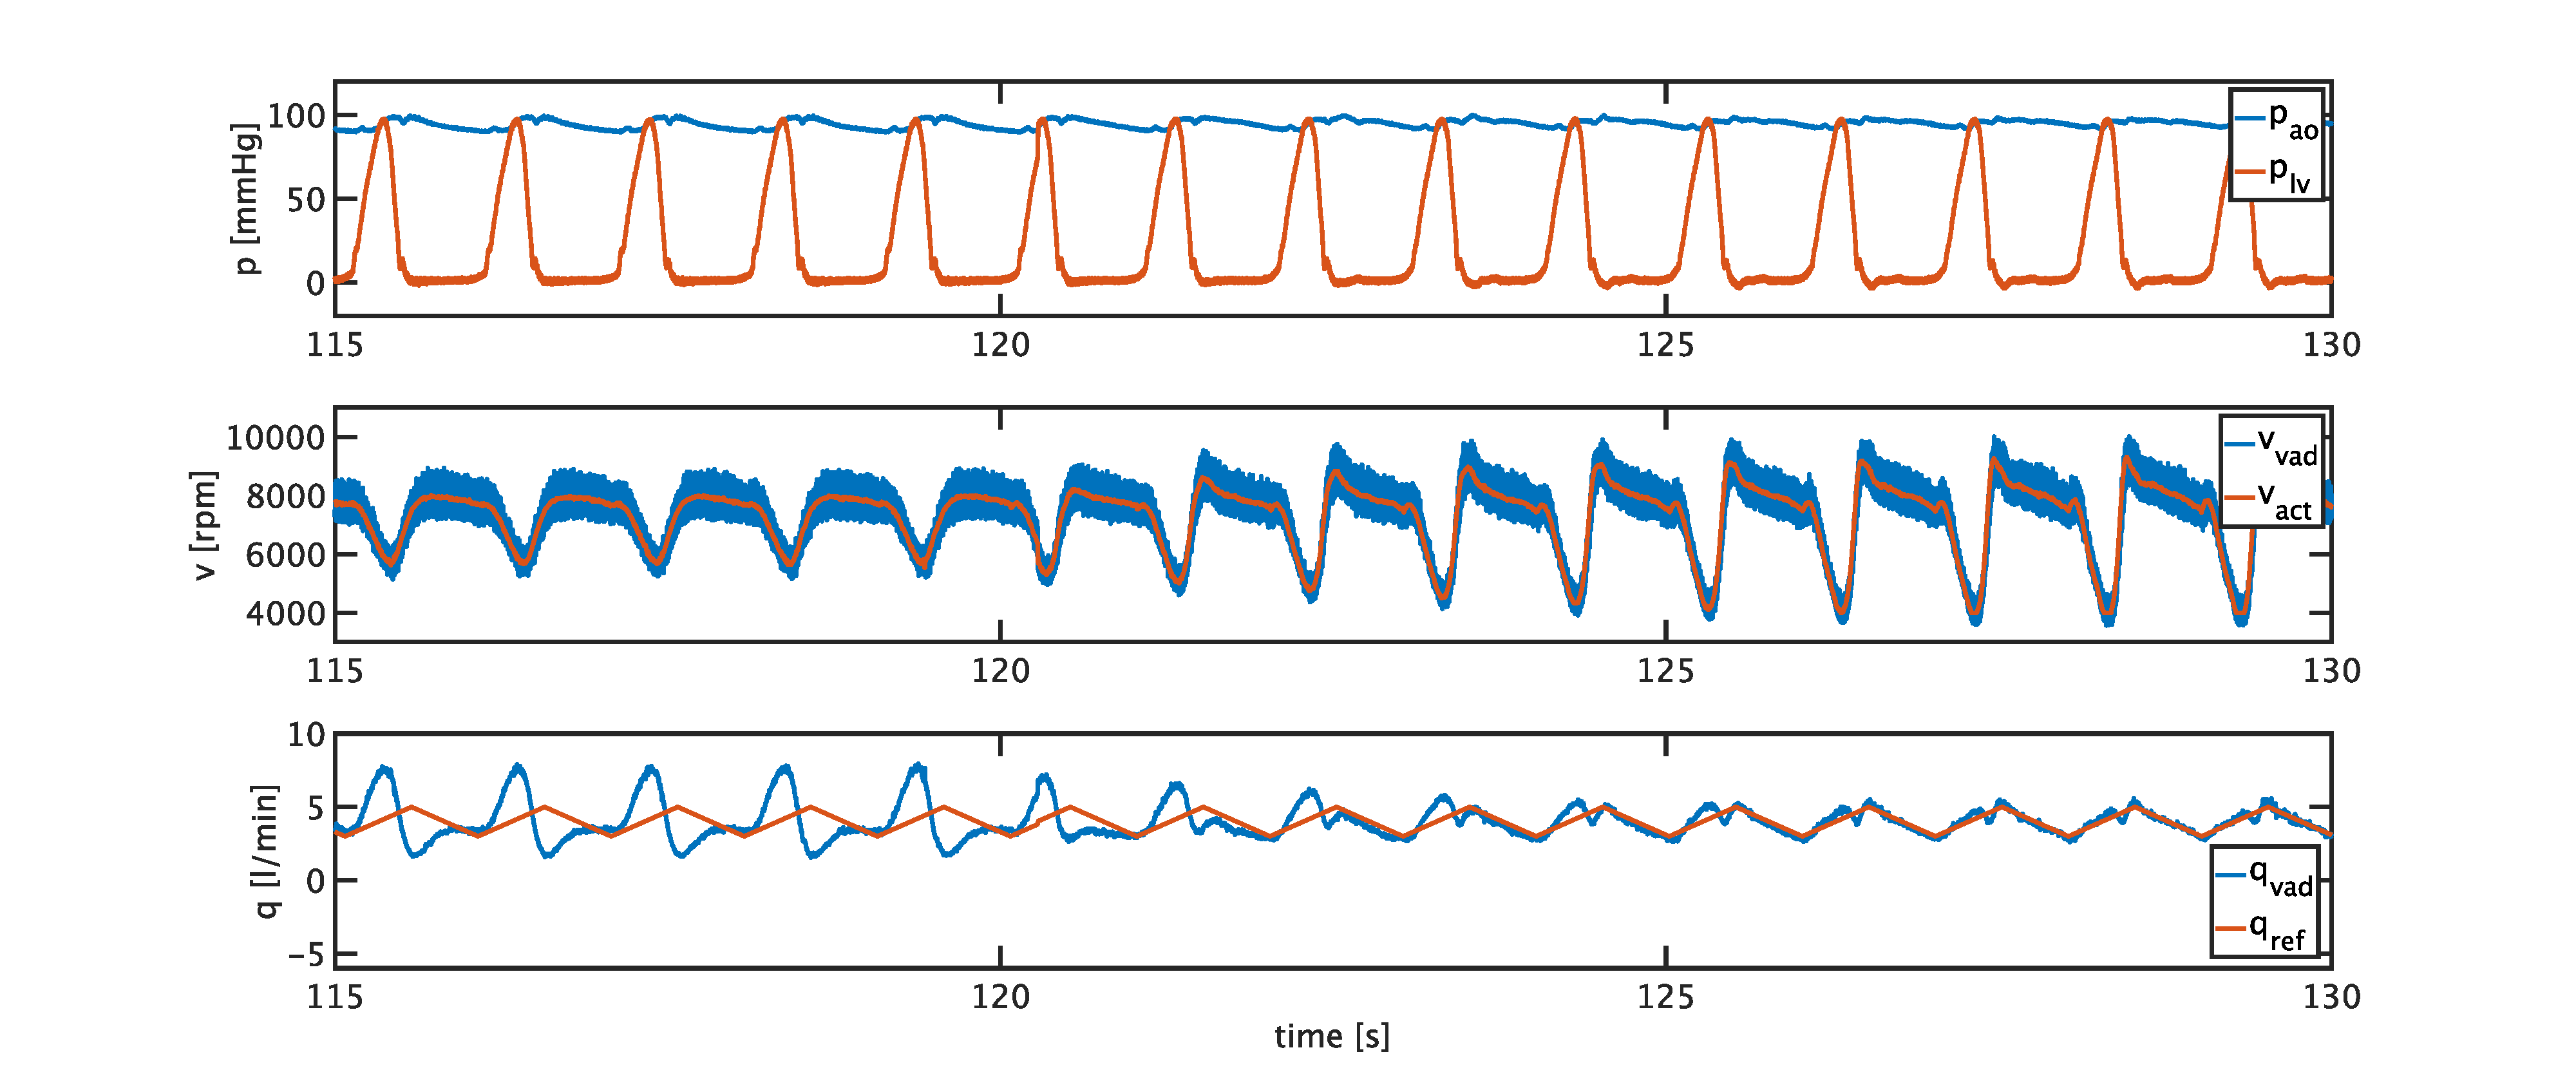
\includegraphics[width=0.95\textwidth]{images/chapt_5/ILC/pi_to_ilc_dist_triang_cf50.pdf}
  \caption[]{Segment of measurement for ILC with disturbance of $HR=60\,bpm$ with $cf_{\mathrm{Lv}}=0.5$ for triangular reference flow. Top:  pressure values of the MCL. Middle: actuating variable and measured rotational speed of the VAD. Bottom: targeted flow trajectory and measured flow through the VAD}
  \label{fig:pi_to_ilc_dist_triang_cf50}
\end{figure}
This is endorsed by comparison of the RMSE values as shown in \figurename~\ref{fig:RMSE_dist_triang_var_cf}. While RMSE for the PI controller segments lie at $RMSE_{\mathrm{PI,triang,cf_{\mathrm{Lv}}=0.5}}\approx 1.9\, l/min$ and $RMSE_{\mathrm{PI,triang,cf_{\mathrm{Lv}}=0.25}}\approx 1.2\, l/min$, the RMSE for the combined control structure amounts to
\begin{equation}
  RMSE_{\mathrm{ILC,triang}}\approx 0.11\, l/min.
\end{equation}
\begin{figure}[ht!]
  \centering
  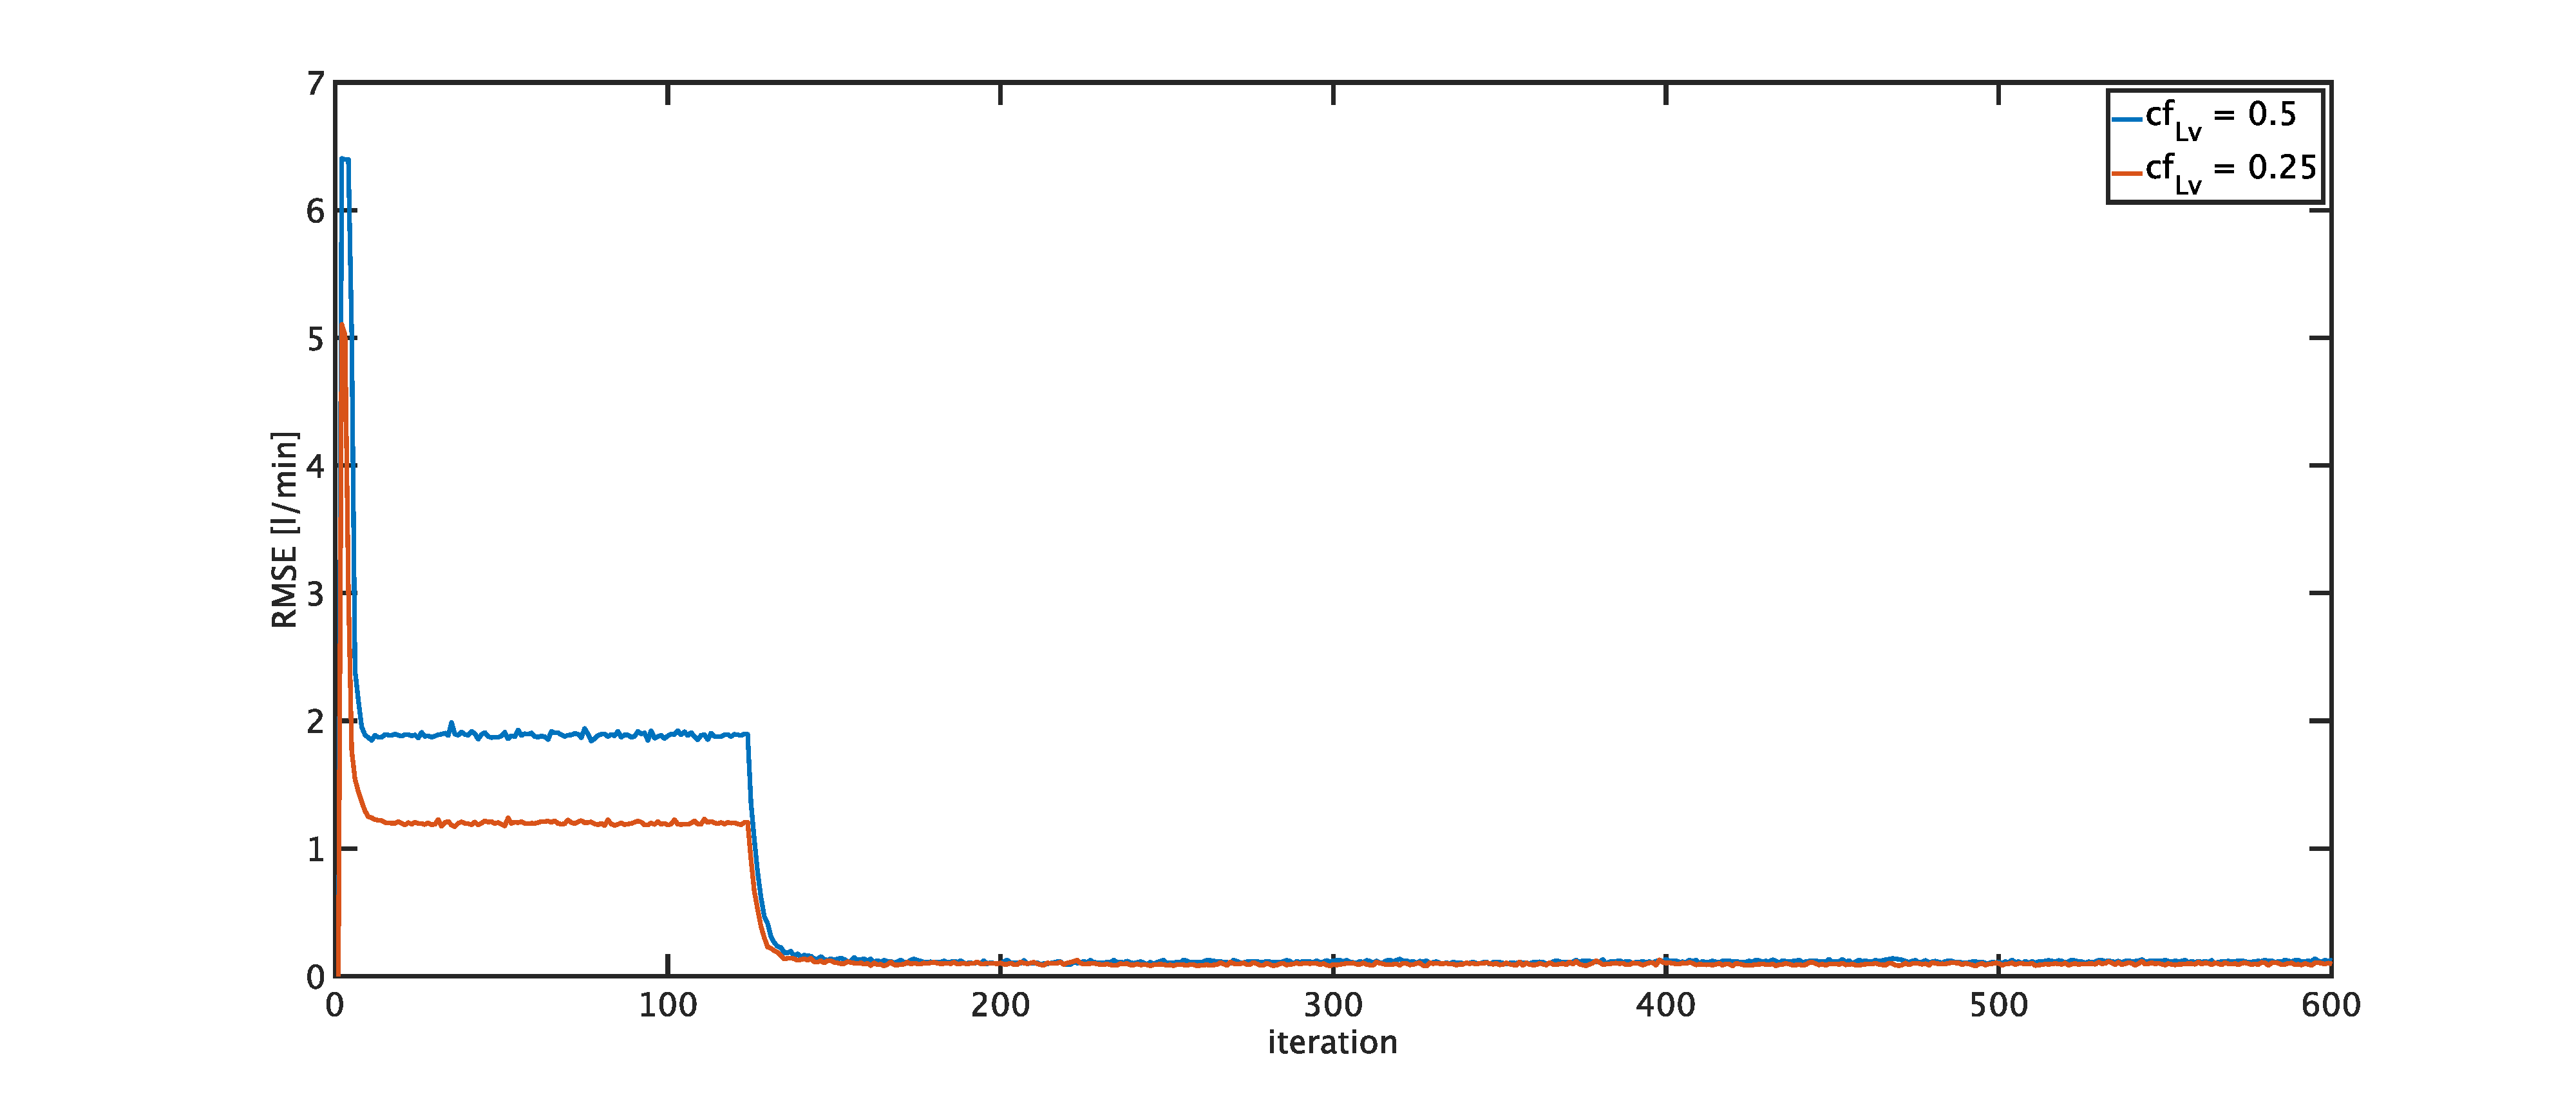
\includegraphics[width=0.95\textwidth]{images/chapt_5/ILC/RMSE_dist_triang_var_cf.pdf}
  \caption[RMSE Comparison of ILC at triangular reference flow for varying left ventricular contractilities]{Comparison of RMSE values of the ILC for triangular reference flow with disturbance of $HR=60\,bpm$ for varying contractility values of the left ventricle.}
  \label{fig:RMSE_dist_triang_var_cf}
\end{figure}

The last measurements for analysis of controller performance of the ILC subjected to a repeating disturbance are performed using the rectangular reference trajectory. As in all previous measurements, the exclusive use of the PI controller is not suitable to track the reference. Combined control however, once more shows adjustment to the reference in a few iterations. \figurename~\ref{fig:pi_to_ilc_dist_square_60_cf1} depicts the course of pressure in the aorta and left ventricle, the actuating variable and the rotational speed of the VAD as well as the reference trajectory and the actually achieve flow through the VAD for the transitional segment of the measurement at $cf_{\mathrm{Lv}}=1$.
\begin{figure}[ht!]
  \centering
  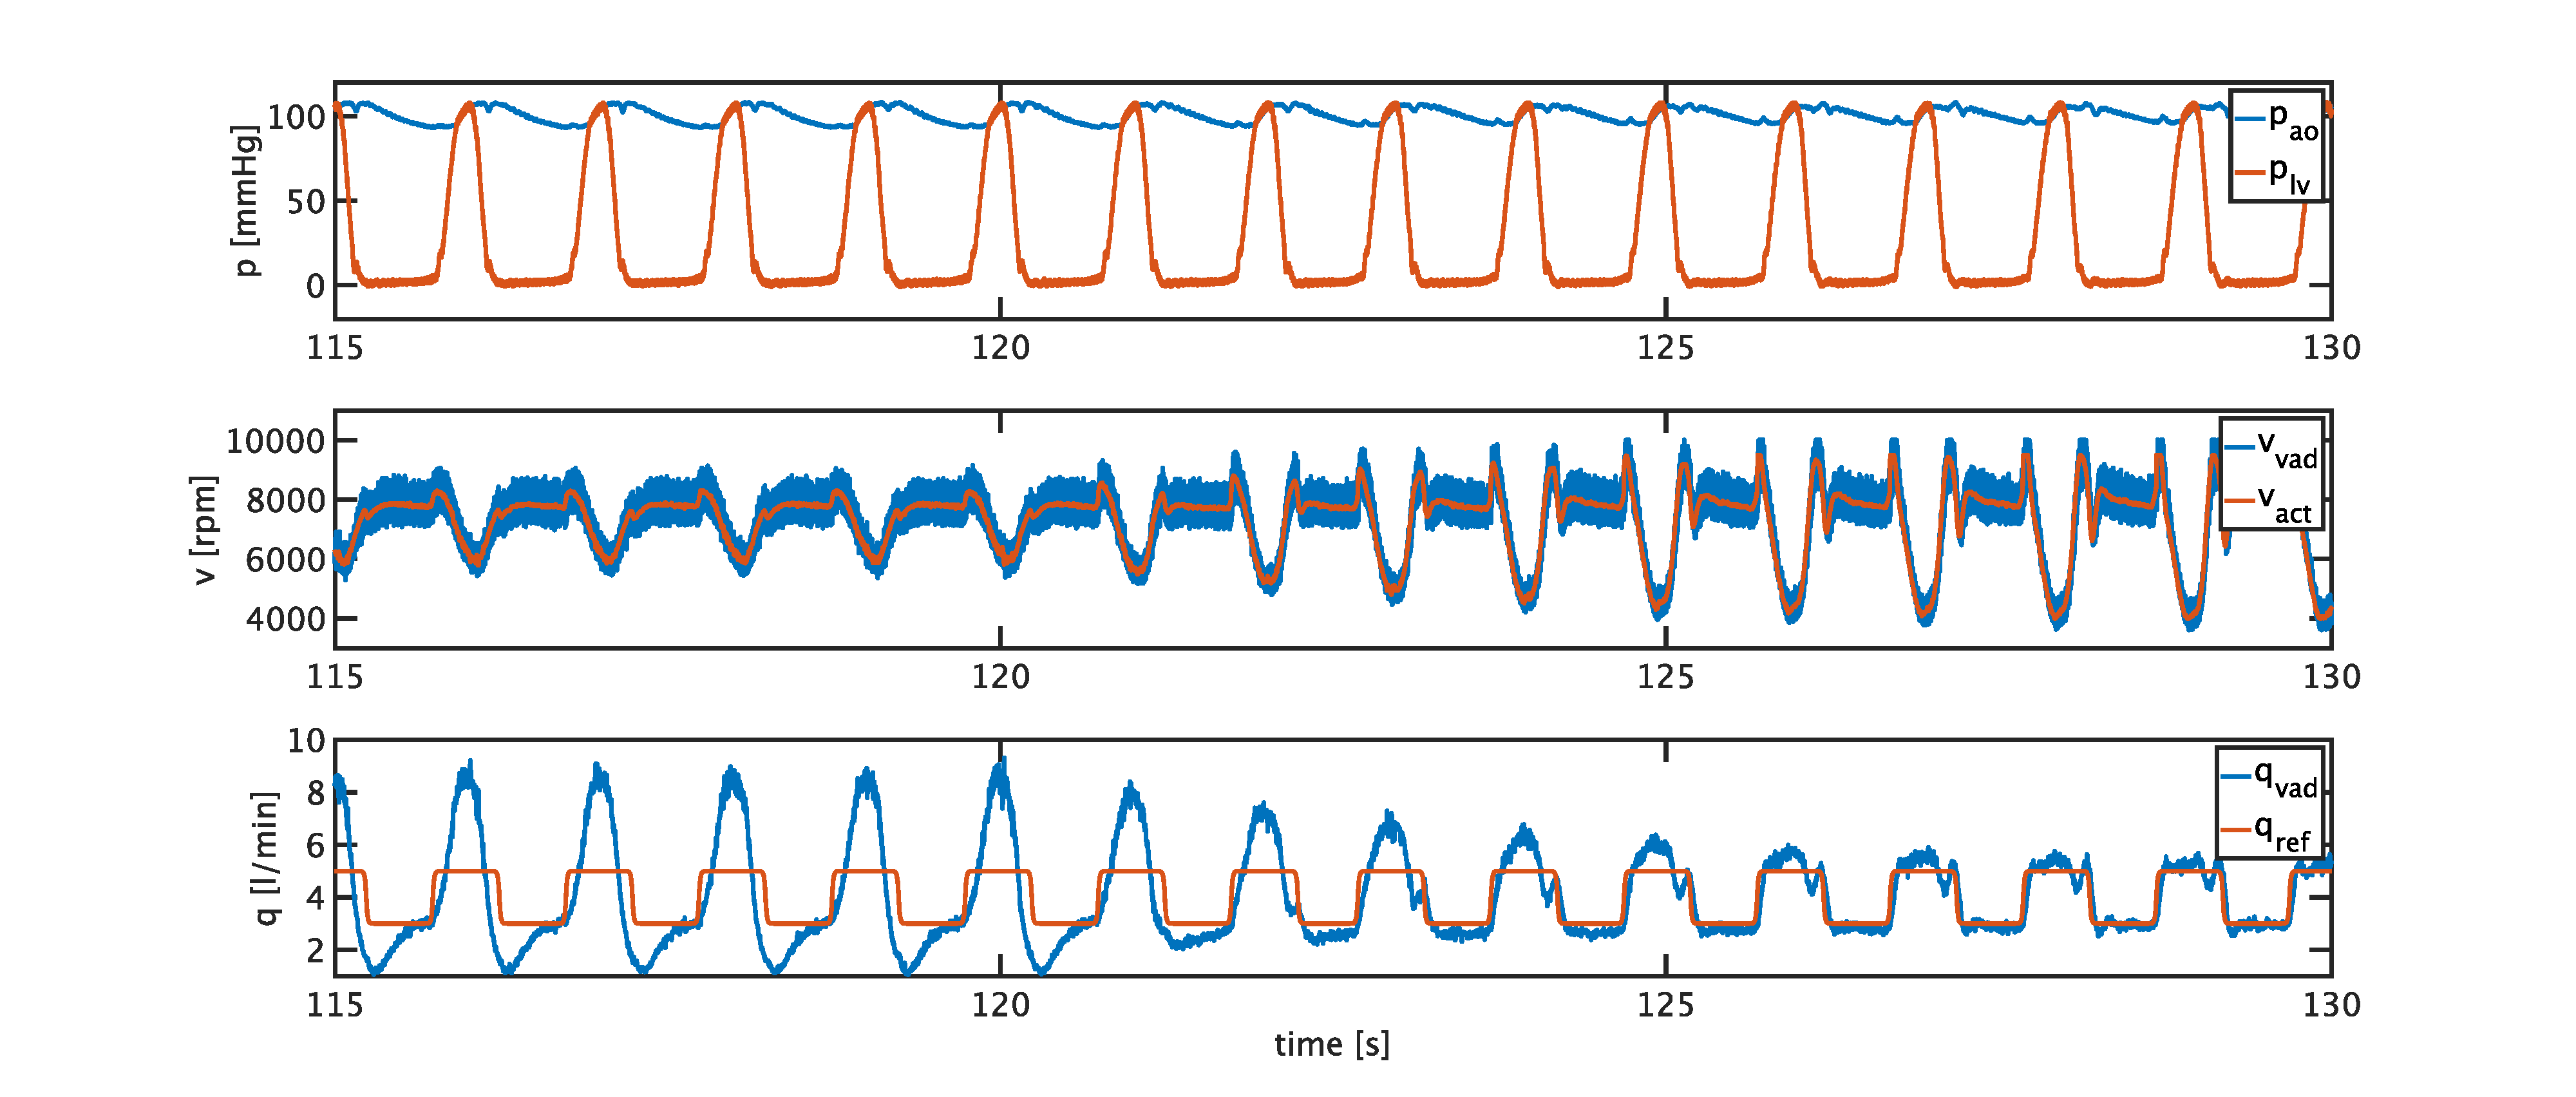
\includegraphics[width=0.95\textwidth]{images/chapt_5/ILC/pi_to_ilc_dist_square_60_cf1.pdf}
  \caption[Segment of measurement for ILC with disturbance of $HR=60\,bpm$ with $cf_{\mathrm{Lv}}=1$ for rectangular reference flow]{Segment of measurement for ILC with disturbance of $HR=60\,bpm$ with $cf_{\mathrm{Lv}}=1$ for rectangular reference flow. Top:  pressure values of the MCL. Middle: actuating variable and measured rotational speed of the VAD. Bottom: targeted flow trajectory and measured flow through the VAD}
  \label{fig:pi_to_ilc_dist_square_60_cf1}
\end{figure}
\\The comparison of RMSE courses for all four left ventricular contractility levels is depicted in \figurename~\ref{fig:RMSE_dist_square_60_var_cf}. Once more, contractility decrease directly influences the performance of the PI controller while the end value for RMSE of the ILC for all contractility levels amounts to
\begin{equation}
  RMSE_{\mathrm{ILC,rect}}\approx 0.22\,l/min.
\end{equation}
\begin{figure}[ht!]
  \centering
  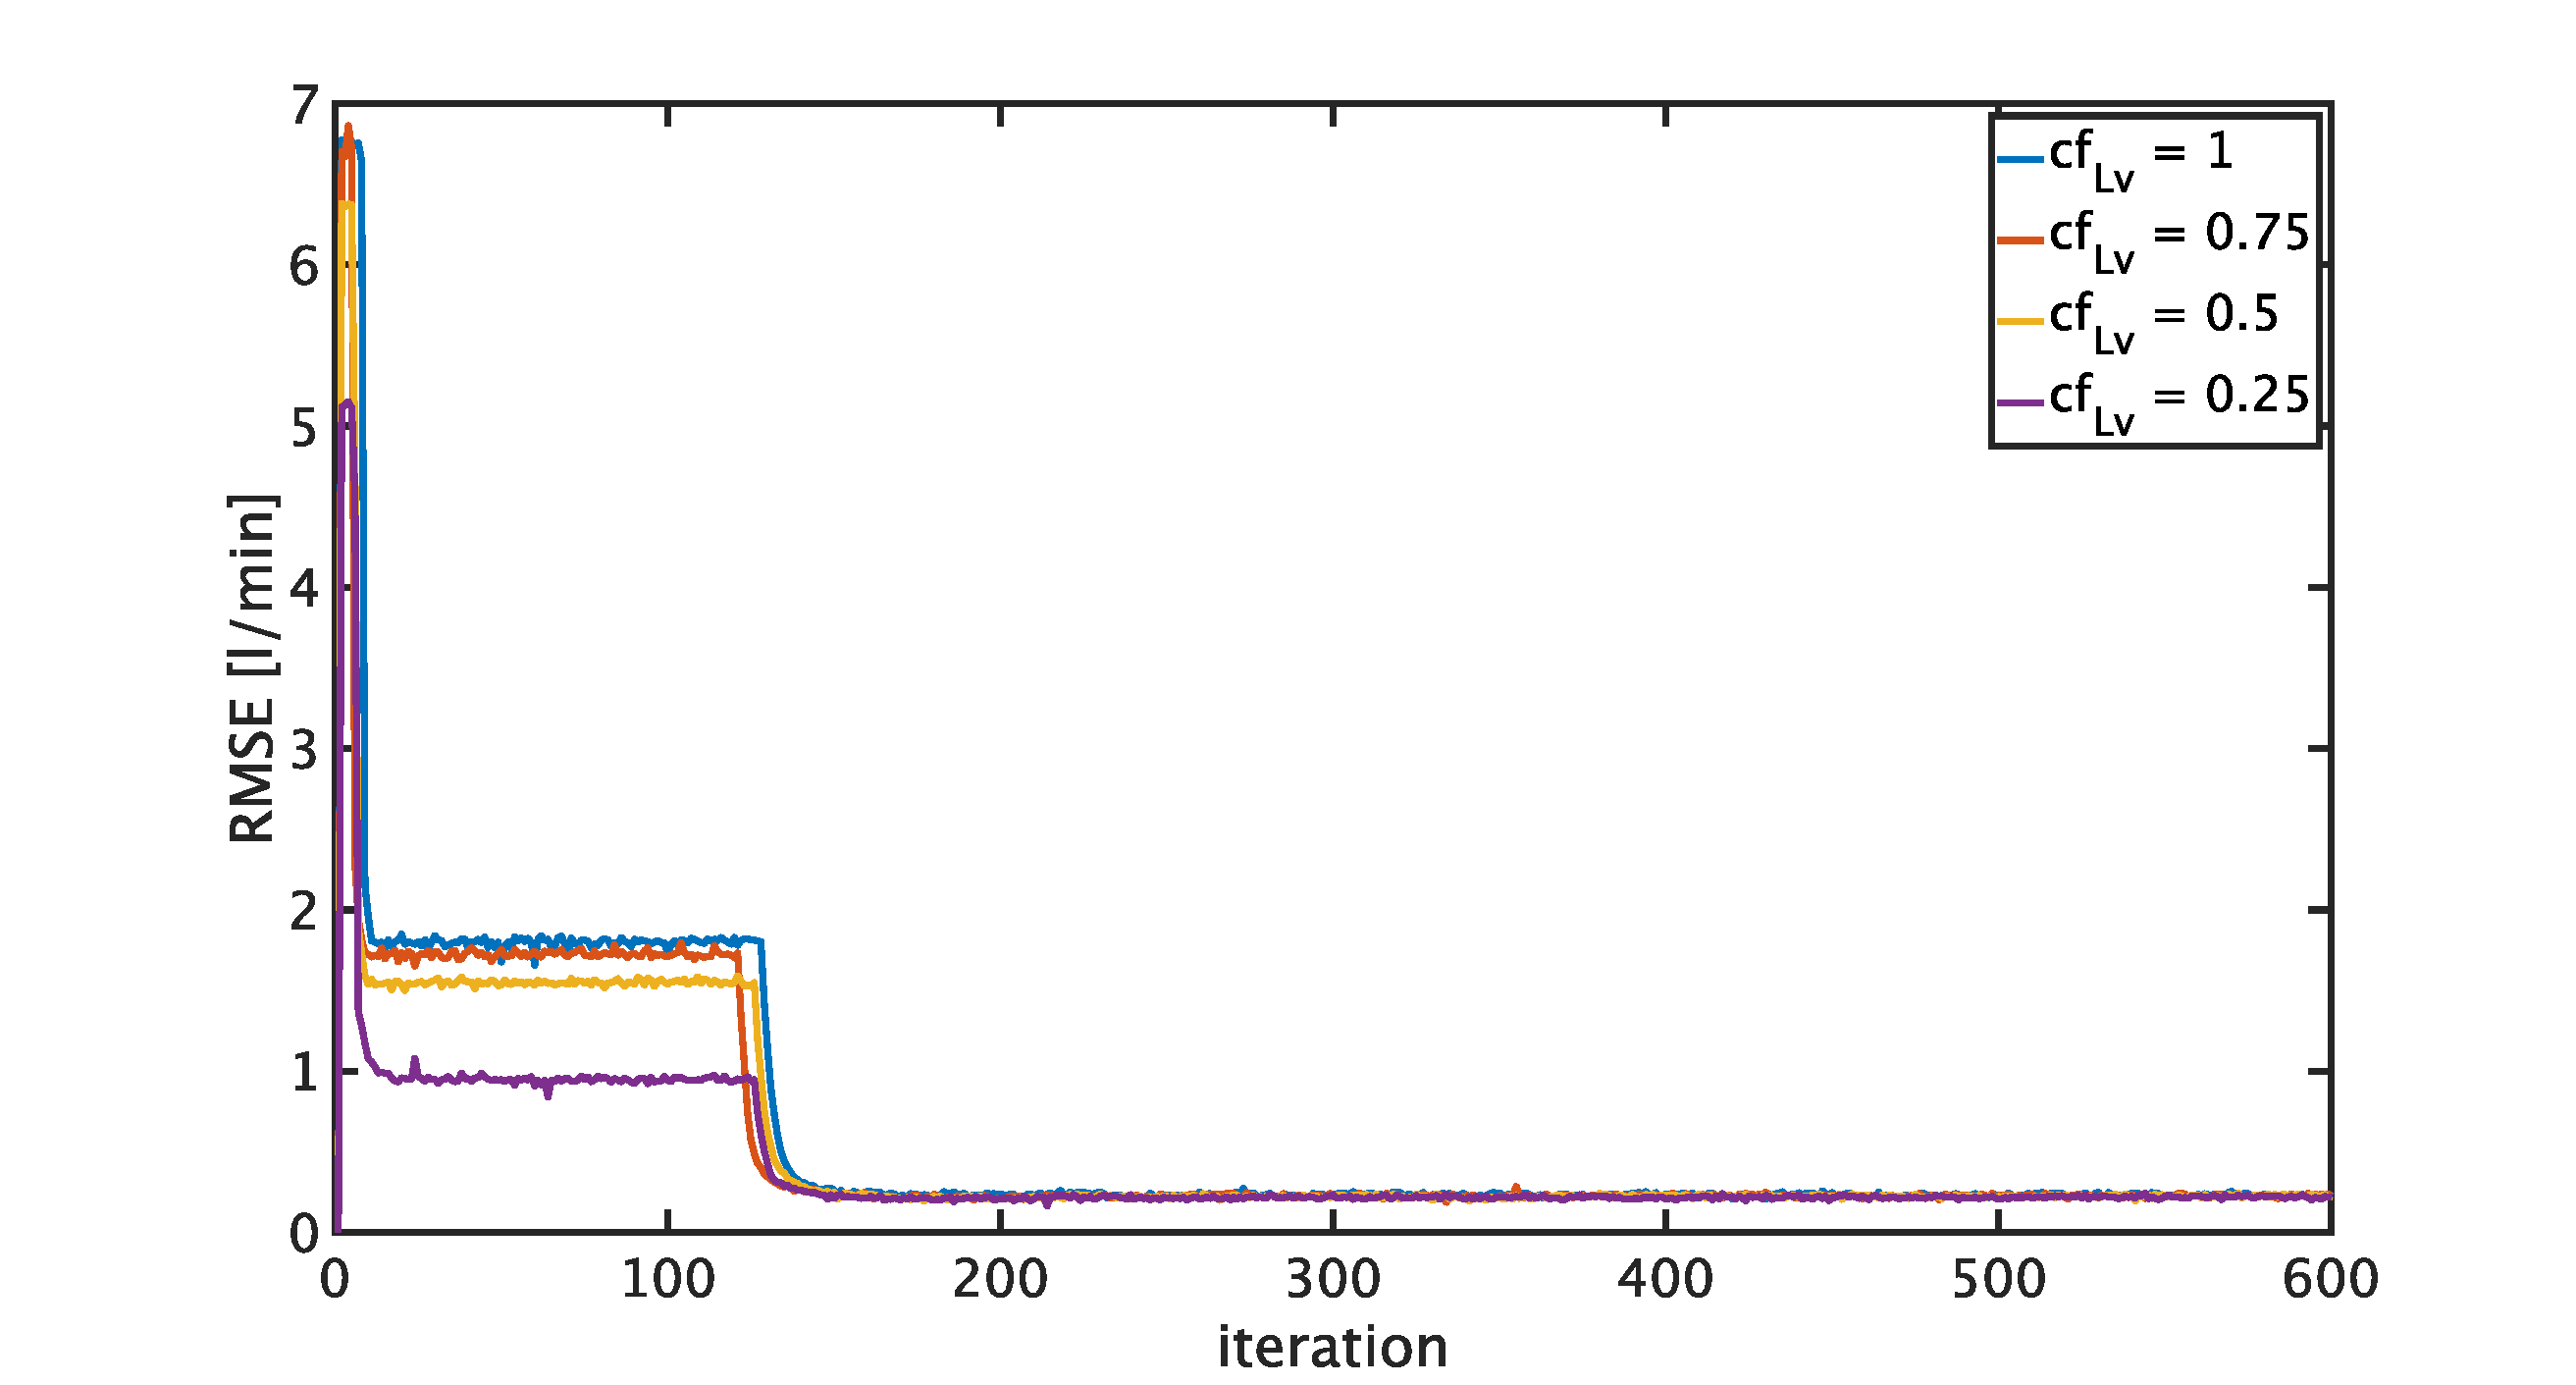
\includegraphics[width=0.95\textwidth]{images/chapt_5/ILC/RMSE_dist_square_60_var_cf.pdf}
  \caption[RMSE Comparison of ILC for a rectangular reference flow for varying left ventricular contractilities]{Comparison of RMSE values of the ILC for rectangular reference flow with disturbance of $HR=60\,bpm$ for varying contractility values of the left ventricle.}
  \label{fig:RMSE_dist_square_60_var_cf}
\end{figure}
\\To prepare measurements considering different disturbances, in addition to measurements considering different contractility values for the left ventricle, measurements are performed at several heart rates for the rectangular reference. Heart rate is defined in four steps of $20\,bpm$ from $HR=40\,bpm$ to $HR=100\,bpm$. All of these measurements show stable behavior throughout the complete measurement time of $500\,s$.
Looking at \figurename~\ref{fig:RMSE_dist_square_const_var_hr}, it can be concluded that the performance of the PI controller improves only for the slowest heart rate of $HR=40\,bpm$ compared to the rest. Also the results for the RMSE of the ILC control show that the control for a disturbance with $HR=40\,bpm$ with
\begin{equation}
  RMSE_{\mathrm{ILC,40bpm}}\approx 0.16\,l/min
\end{equation}
succeeds the results for the other three heart rates with
\begin{equation}
  RMSE_{\mathrm{ILC,60/80/100bpm}}\approx 0.22\,l/min.
\end{equation}
\begin{figure}[ht!]
  \centering
  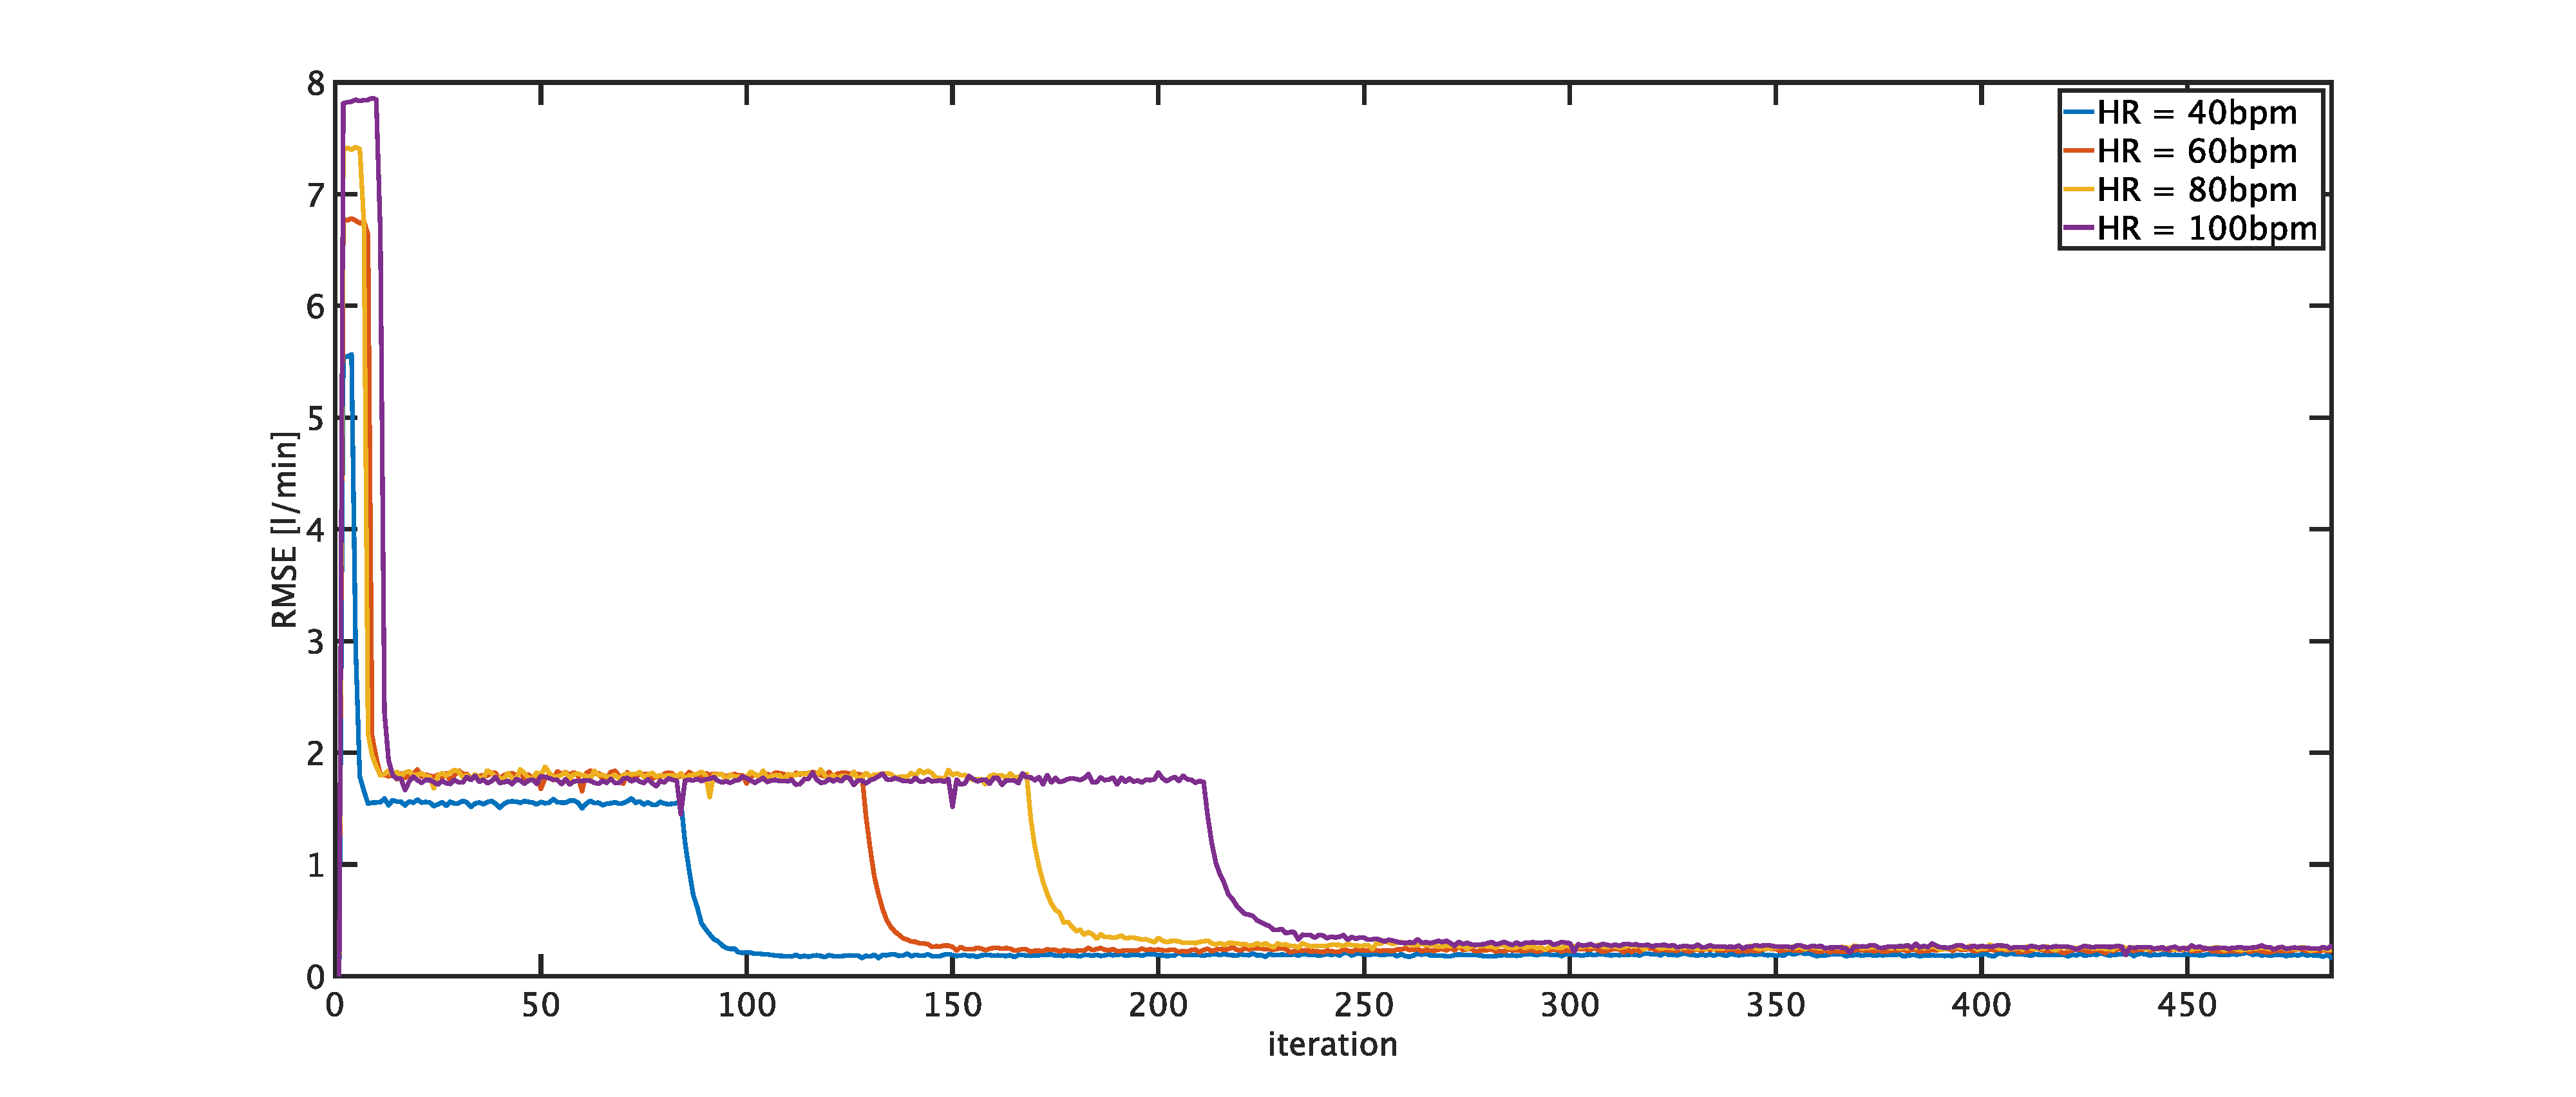
\includegraphics[width=0.95\textwidth]{images/chapt_5/ILC/RMSE_dist_square_const_var_hr.pdf}
  \caption[RMSE Comparison of ILC at rectangular reference flow for varying heart rates]{Comparison of RMSE values of the ILC for rectangular reference flow with $cf_{\mathrm{Lv}}=1$ for varying heart rates.}
  \label{fig:RMSE_dist_square_const_var_hr}
\end{figure}
\\However, the results indicate that using ILC control is a suitable option for all of these heart rates.
\section{Iterative Learning Control with varying disturbance}
Due to the fact that a person's heartbeat does not always occur at a uniform heart rate, but is subject to fluctuations, the ILC is tested for use in suppressing varying disturbances.

\subsection{Design and Implementation}
As the standard P-type ILC is not set up for use under the influence of non repeating disturbances some changes have to be implemented.
\\To perform the tests under the influence of changing disturbances, an additional function programmed in Matlab is added to the Simulink model. This allows a constant variation of the heart rate. The function is designed in such a way that by receiving the trigger signal of a new heartbeat, a new heart rate is determined and passed on to the mock circulatory loop and the ILC. In addition to the trigger signal, the function has three more inputs in the form of an upper and lower limit of the heart rate and a step size for a variation of the heart rate. These variables can be set via ControlDesk before starting the measurement.
Starting at the lower limit, the heart rate is increased by the defined step size with each heartbeat until the upper limit of the heart rate is reached. Then, with each heartbeat, the heart rate is decreased by the step size until the lower limit is reached. This is repeated until the measurement is stopped. An example of this sequence with a lower limit of $60\, bpm$, a step size of $1\, bpm$ and an upper limit of $100\, bpm$ is shown in \figurename~\ref{fig:hr_increase}.
\begin{figure}[ht!]
  \centering
  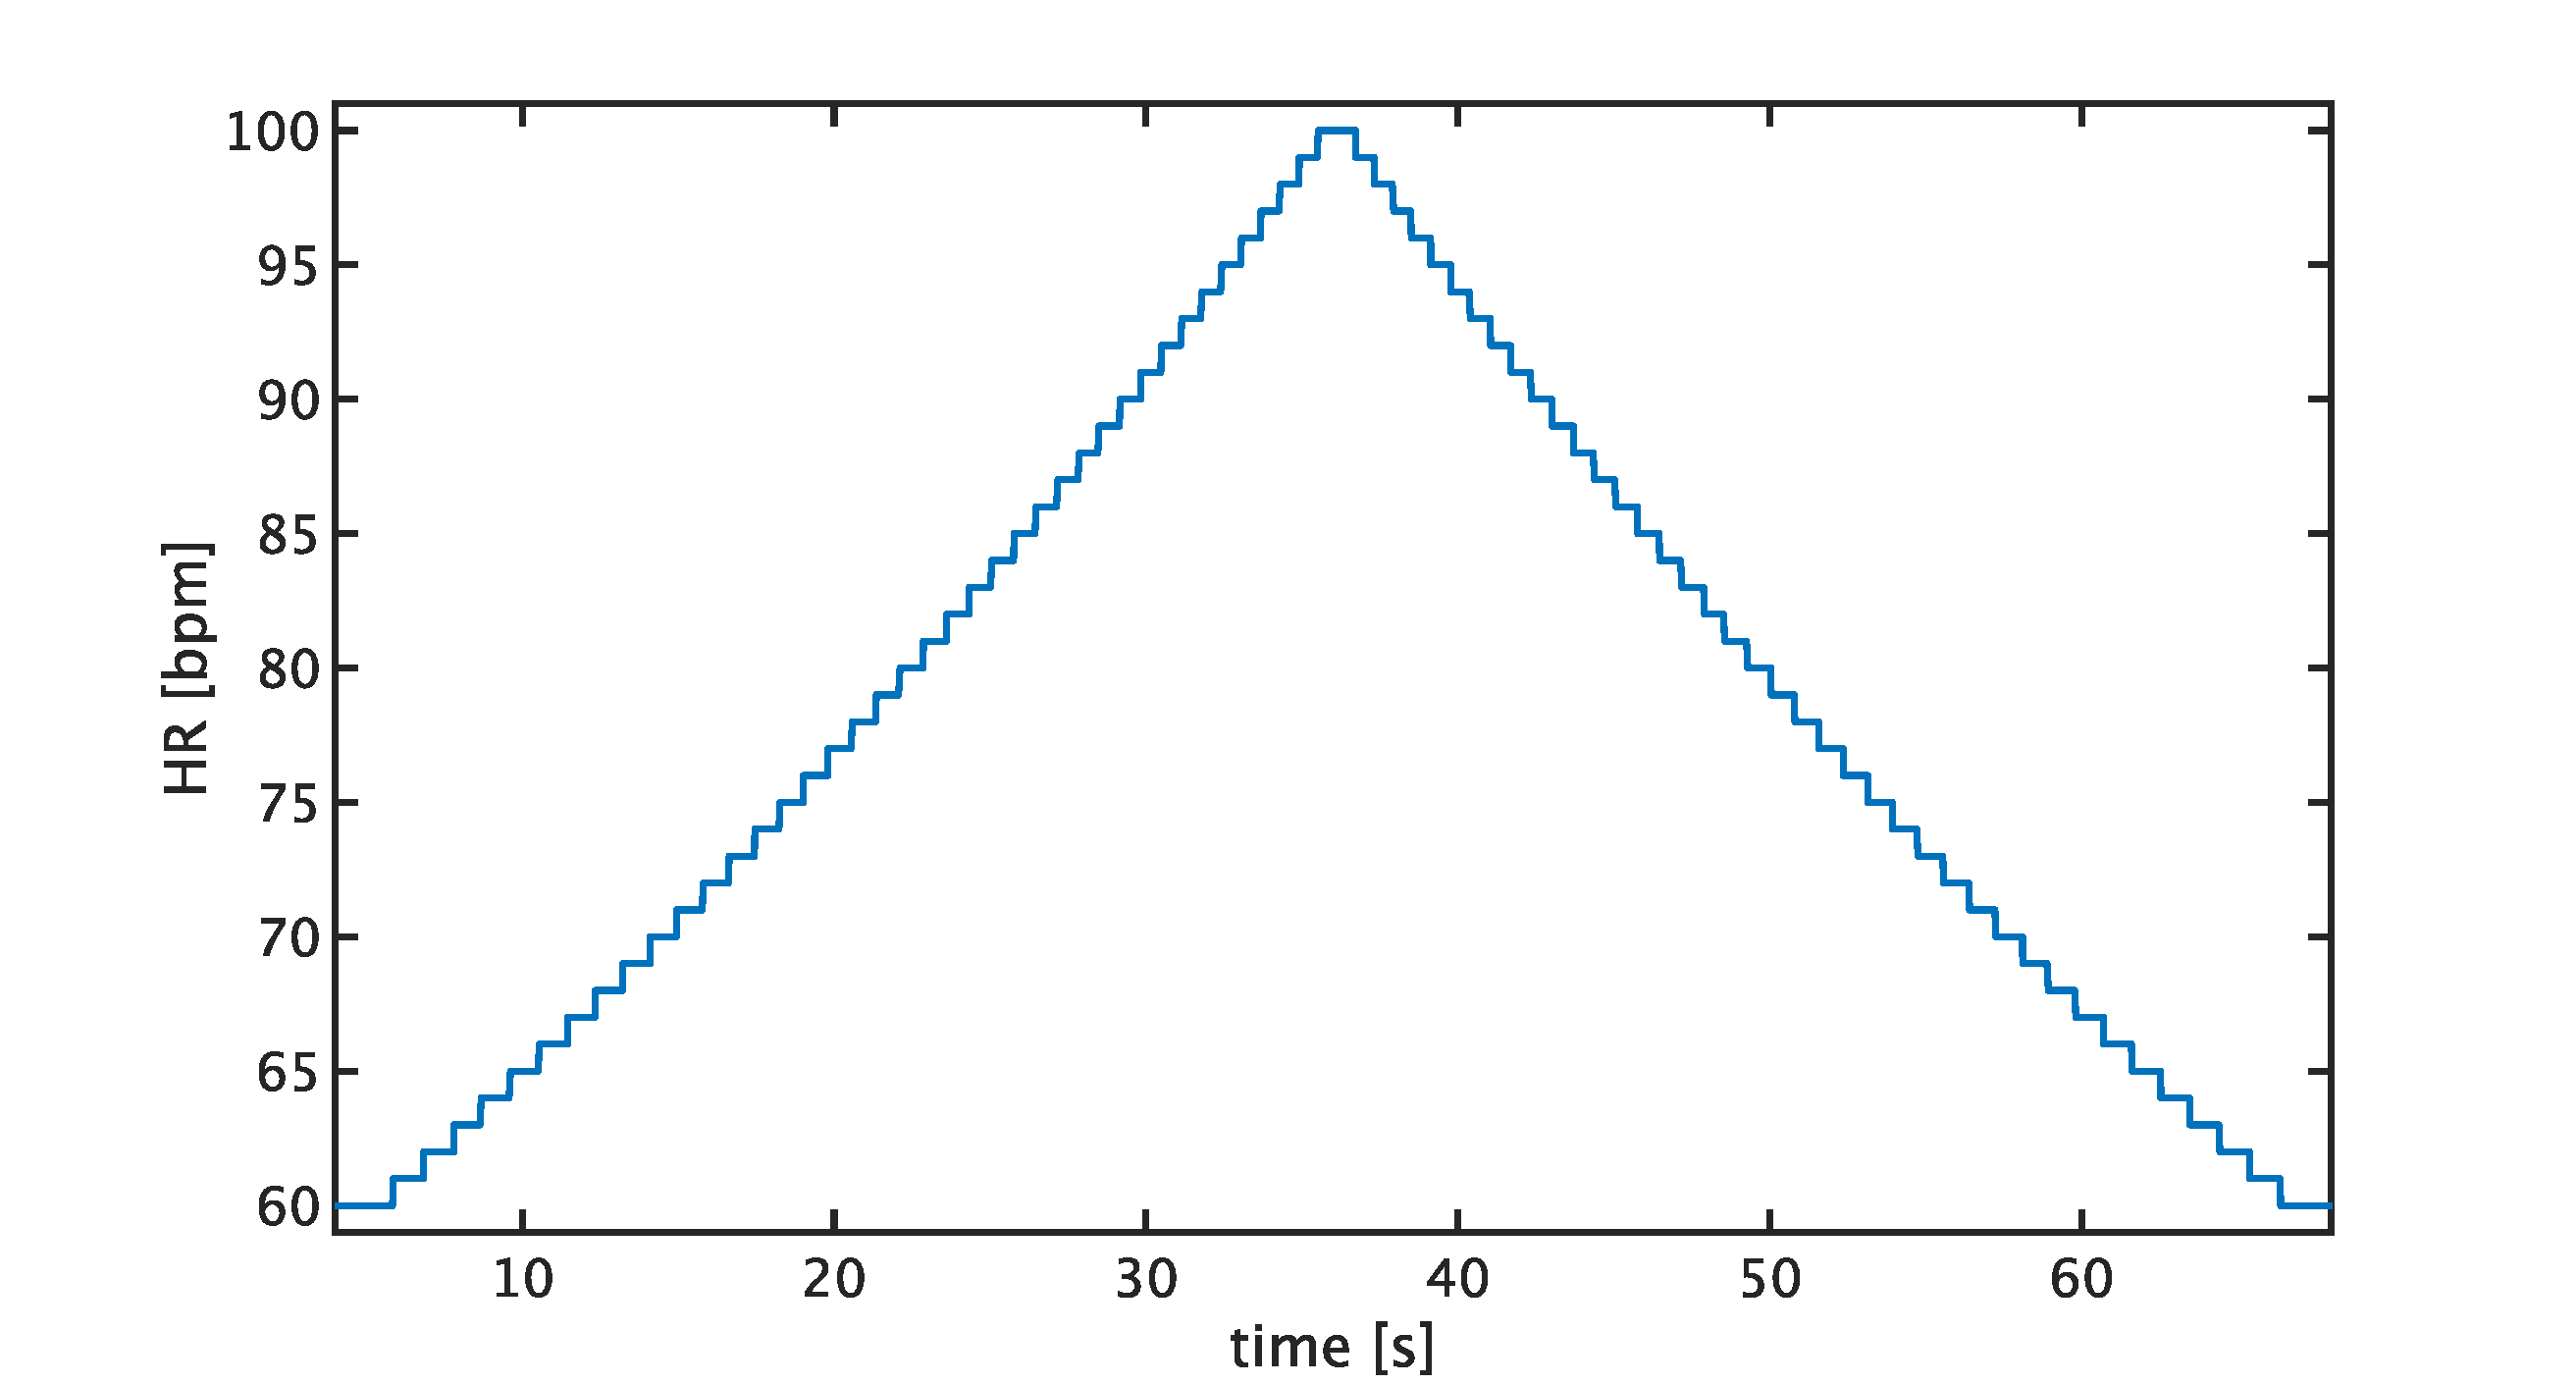
\includegraphics[width=0.95\textwidth]{images/chapt_5/ILC/hr_increase.pdf}
  \caption[Illustration of HR change]{Illustration of HR change.}
  \label{fig:hr_increase}
\end{figure}


Since the variation of the heart rate leads to changing iteration duration an additional preprocessing step is implemented within the ILC function. This introduces a functionality which allows to resample the stored data of the previous iteration and adapt it to the duration of the current iteration. This process is performed after the data filtering step of the ILC, before the data is output to the control loop.
\\To adjust resampling of the data to the length of the , knowledge of the heart rates is required. Within the tests at the MCL this requirement is fulfilled. For an application on the patient, an additional use of an ECG would be necessary.
The resampling function calculates the iteration length according to
\begin{equation}
  it\_len = \lfloor\frac{60}{HR}\cdot1000\rfloor
\end{equation}
with $HR$ being the heart rate. The duration of the last iteration is stored in the variable $it\_len\_prev$. Using this variable and the current iteration length an index factor is calculated to
\begin{equation}
  idx = \frac{it\_len\_prev}{it\_len}.
\end{equation}
This factor is required to determine the indices of the stored actuating variable values which are to be used to calculate the new values.
In the next step, the lengths of the last and current iteration are compared. In case the iteration times correspond to each other, the stored data are used unchanged for the output to the control loop
\begin{equation}
  \mathbf{u}_{\mathrm{j,ILC}}(i) = \mathbf{u}_{\mathrm{j,ILC,prev}}(i)
\end{equation} for all entries $i$. $\mathbf{u}_{\mathrm{j,ILC,prev}}$ corresponds to the filtered data stored the actuating variable memory during the last iteration while $\mathbf{u}_{\mathrm{j,ILC}}$ represents the data output during the current iteration.
\\Calculation steps for different iteration durations differ only for the first entry. In case the current iteration length is shorter than the last ($it\_len<it\_len\_prev$)
\begin{equation}
  \mathbf{u}_{\mathrm{j,ILC}}(1) = \mathbf{u}_{\mathrm{j,ILC,prev}}(1)
\end{equation} is always valid for the first entry of the actuating variable.
A weighting factor is required for all other entries $i$ of the actuating variable vector to determine resampled data. This is calculated as
\begin{equation}
  weight= i \cdot idx - \lfloor i \cdot idx\rfloor.
\end{equation}
The value for the current entry $i$ is than determined as
\begin{equation}
  \mathbf{u}_{\mathrm{j,ILC}}(i) = (1-weight) \cdot \mathbf{u}_{\mathrm{j,ILC,prev}}(\lfloor i \cdot idx\rfloor) + weight\cdot \mathbf{u}_{\mathrm{j,ILC,prev}}(\lceil i \cdot idx\rceil).
\end{equation}
By using this calculation, the data from the previous iteration is compressed or stretched to the current iteration length accordingly.

\subsection{Evaluation}
In order to determine whether resampling of data improves the ILC performance under varying disturbances, two sets of tests are performed. One without resampling the data under variable disturbances and one using the resampling function described above. The results of the tests are compared with each other.
The reference trajectories described in section \ref{ref_traject} are used to perform the measurements. All measurements considered here are performed assuming a left ventricular contractility of $cf_{\mathrm{Lv}}=1$.


At first, a constant reference flow of $4\,l/min$ is presented to the system. \figurename~\ref{fig:ilc_var_dist_unfix_const} depicts a segment of the measurement without resampling of the actuating variable data representing the transition from exclusive PI control to the combined control approach at $120\,s$. At about $152\,s$ the pump stops due to the steadily oscillating behavior of the actuating variable.
\begin{figure}[ht!]
  \centering
  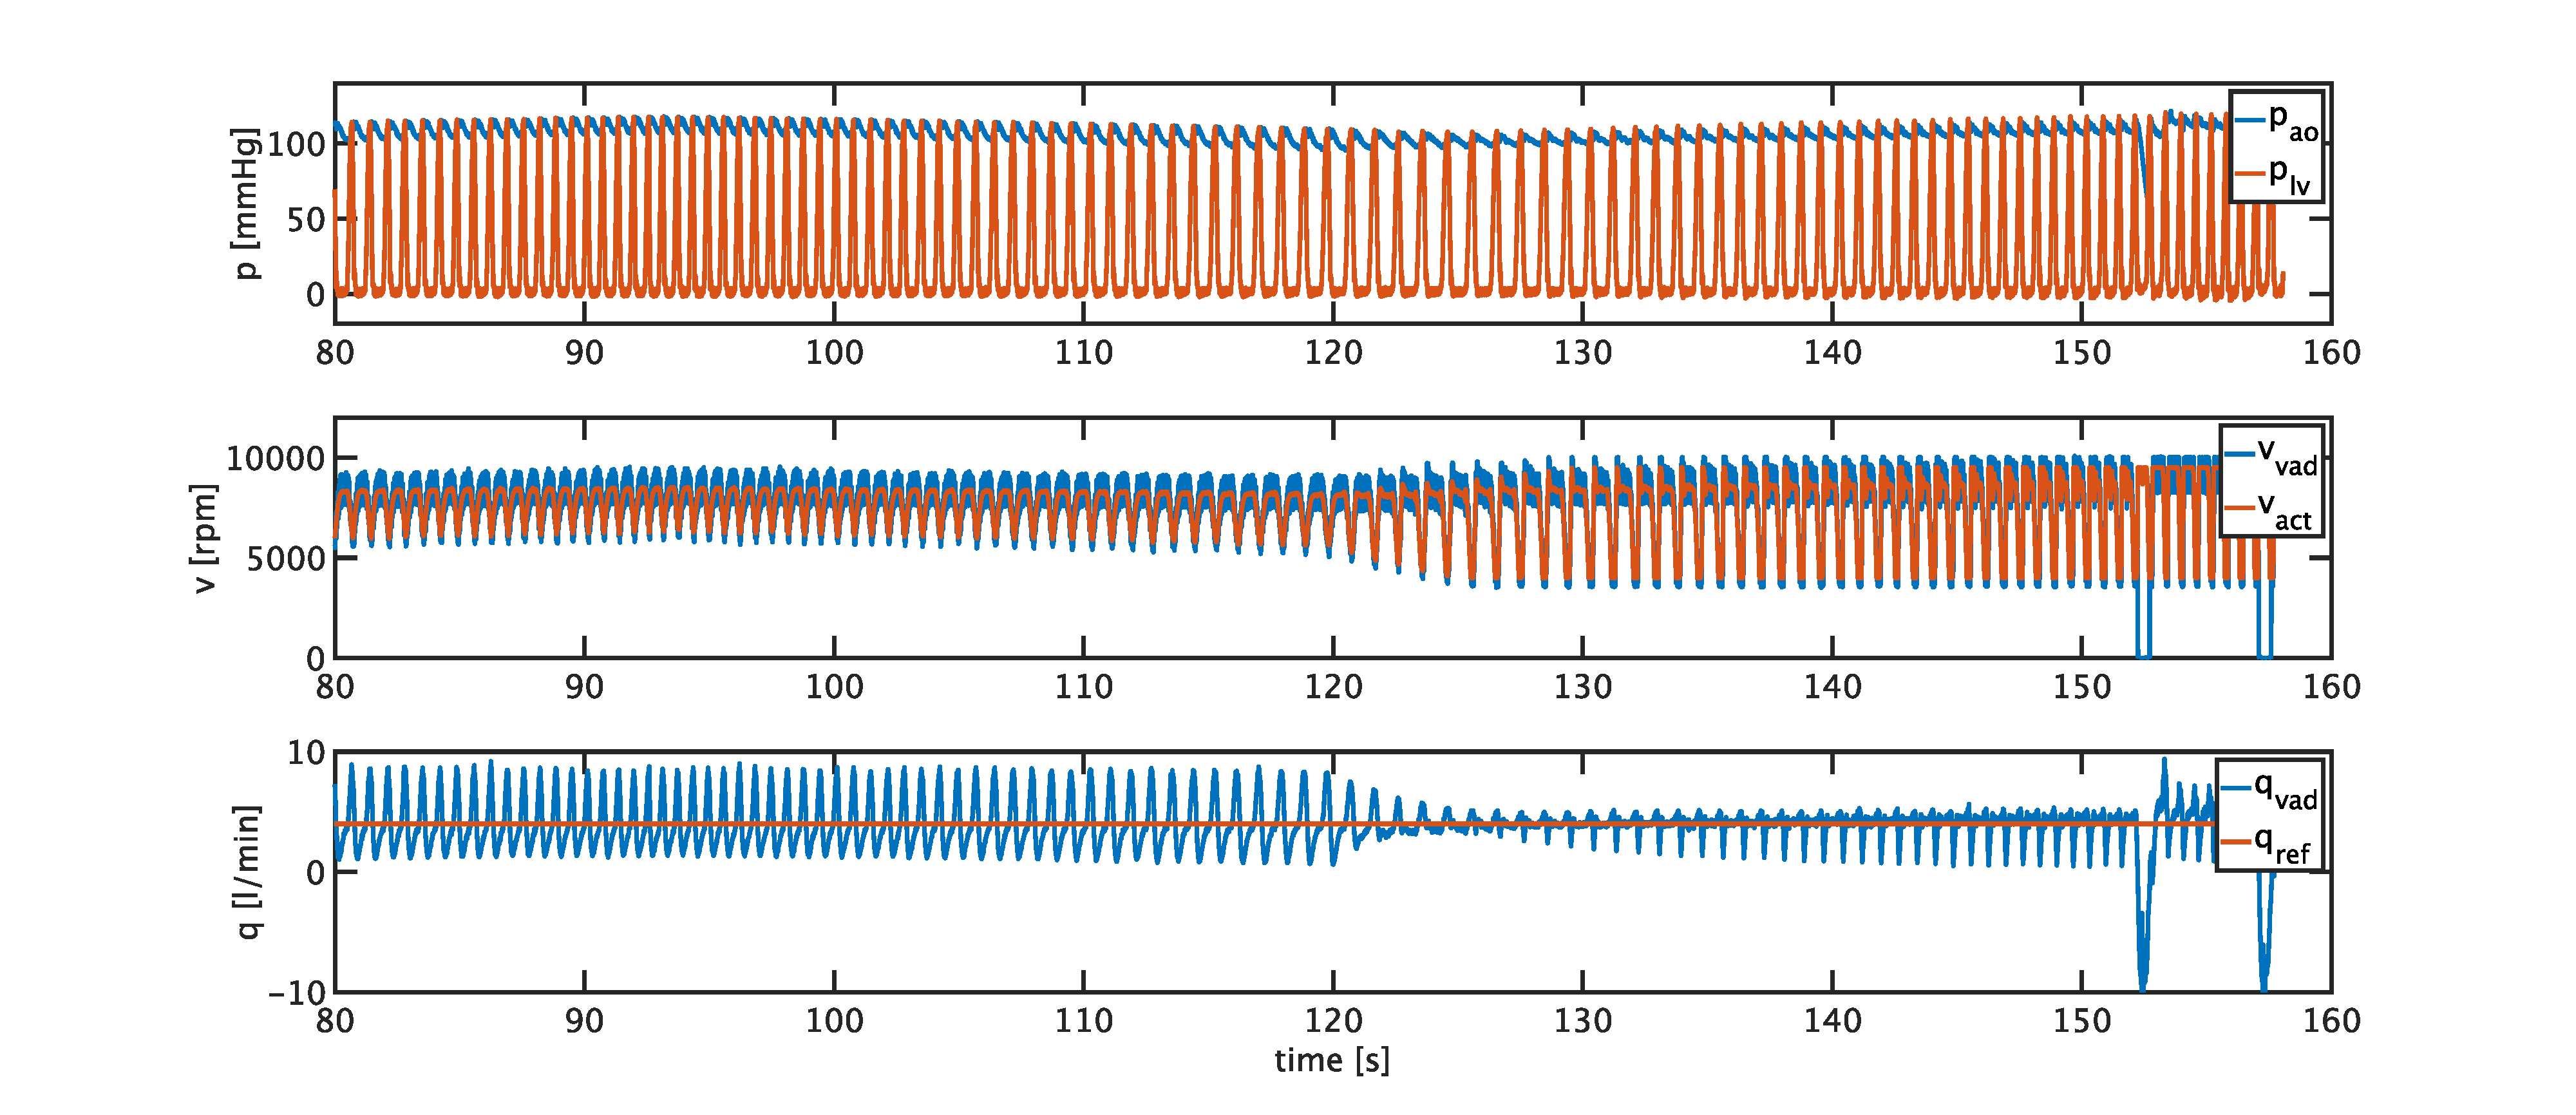
\includegraphics[width=0.95\textwidth]{images/chapt_5/ILC/ilc_var_dist_unfix_const.pdf}
  \caption[Segment of measurement for ILC with varying disturbance with $cf_{\mathrm{Lv}}=1$ for constant reference flow without data resampling]{Segment of measurement for ILC with varying disturbance with $cf_{\mathrm{Lv}}=1$ for constant reference flow without data resampling. Top:  pressure values of the MCL. Middle: actuating variable and measured rotational speed of the VAD. Bottom: targeted flow trajectory and measured flow through the VAD}
  \label{fig:ilc_var_dist_unfix_const}
\end{figure}
As can be seen in \figurename~\ref{fig:ilc_var_dist_fix_const}, similar behavior is observed for the measurement with the resampled actuating variable data.
However, looking at the lower graphs of the two figures, it can be seen that for the unchanged actuating variable data in \figurename~\ref{fig:ilc_var_dist_unfix_const} the measured flow $q_{\mathrm{vad}}$ first approaches the reference, but then moves further away from it again, while the flow through the VAD for the measurement with resampling of the actuating variable data in \figurename~\ref{fig:ilc_var_dist_fix_const} continuously approaches the reference.
\\This suggests a higher performance of the ILC using the resampling functionality.
\begin{figure}[ht!]
  \centering
  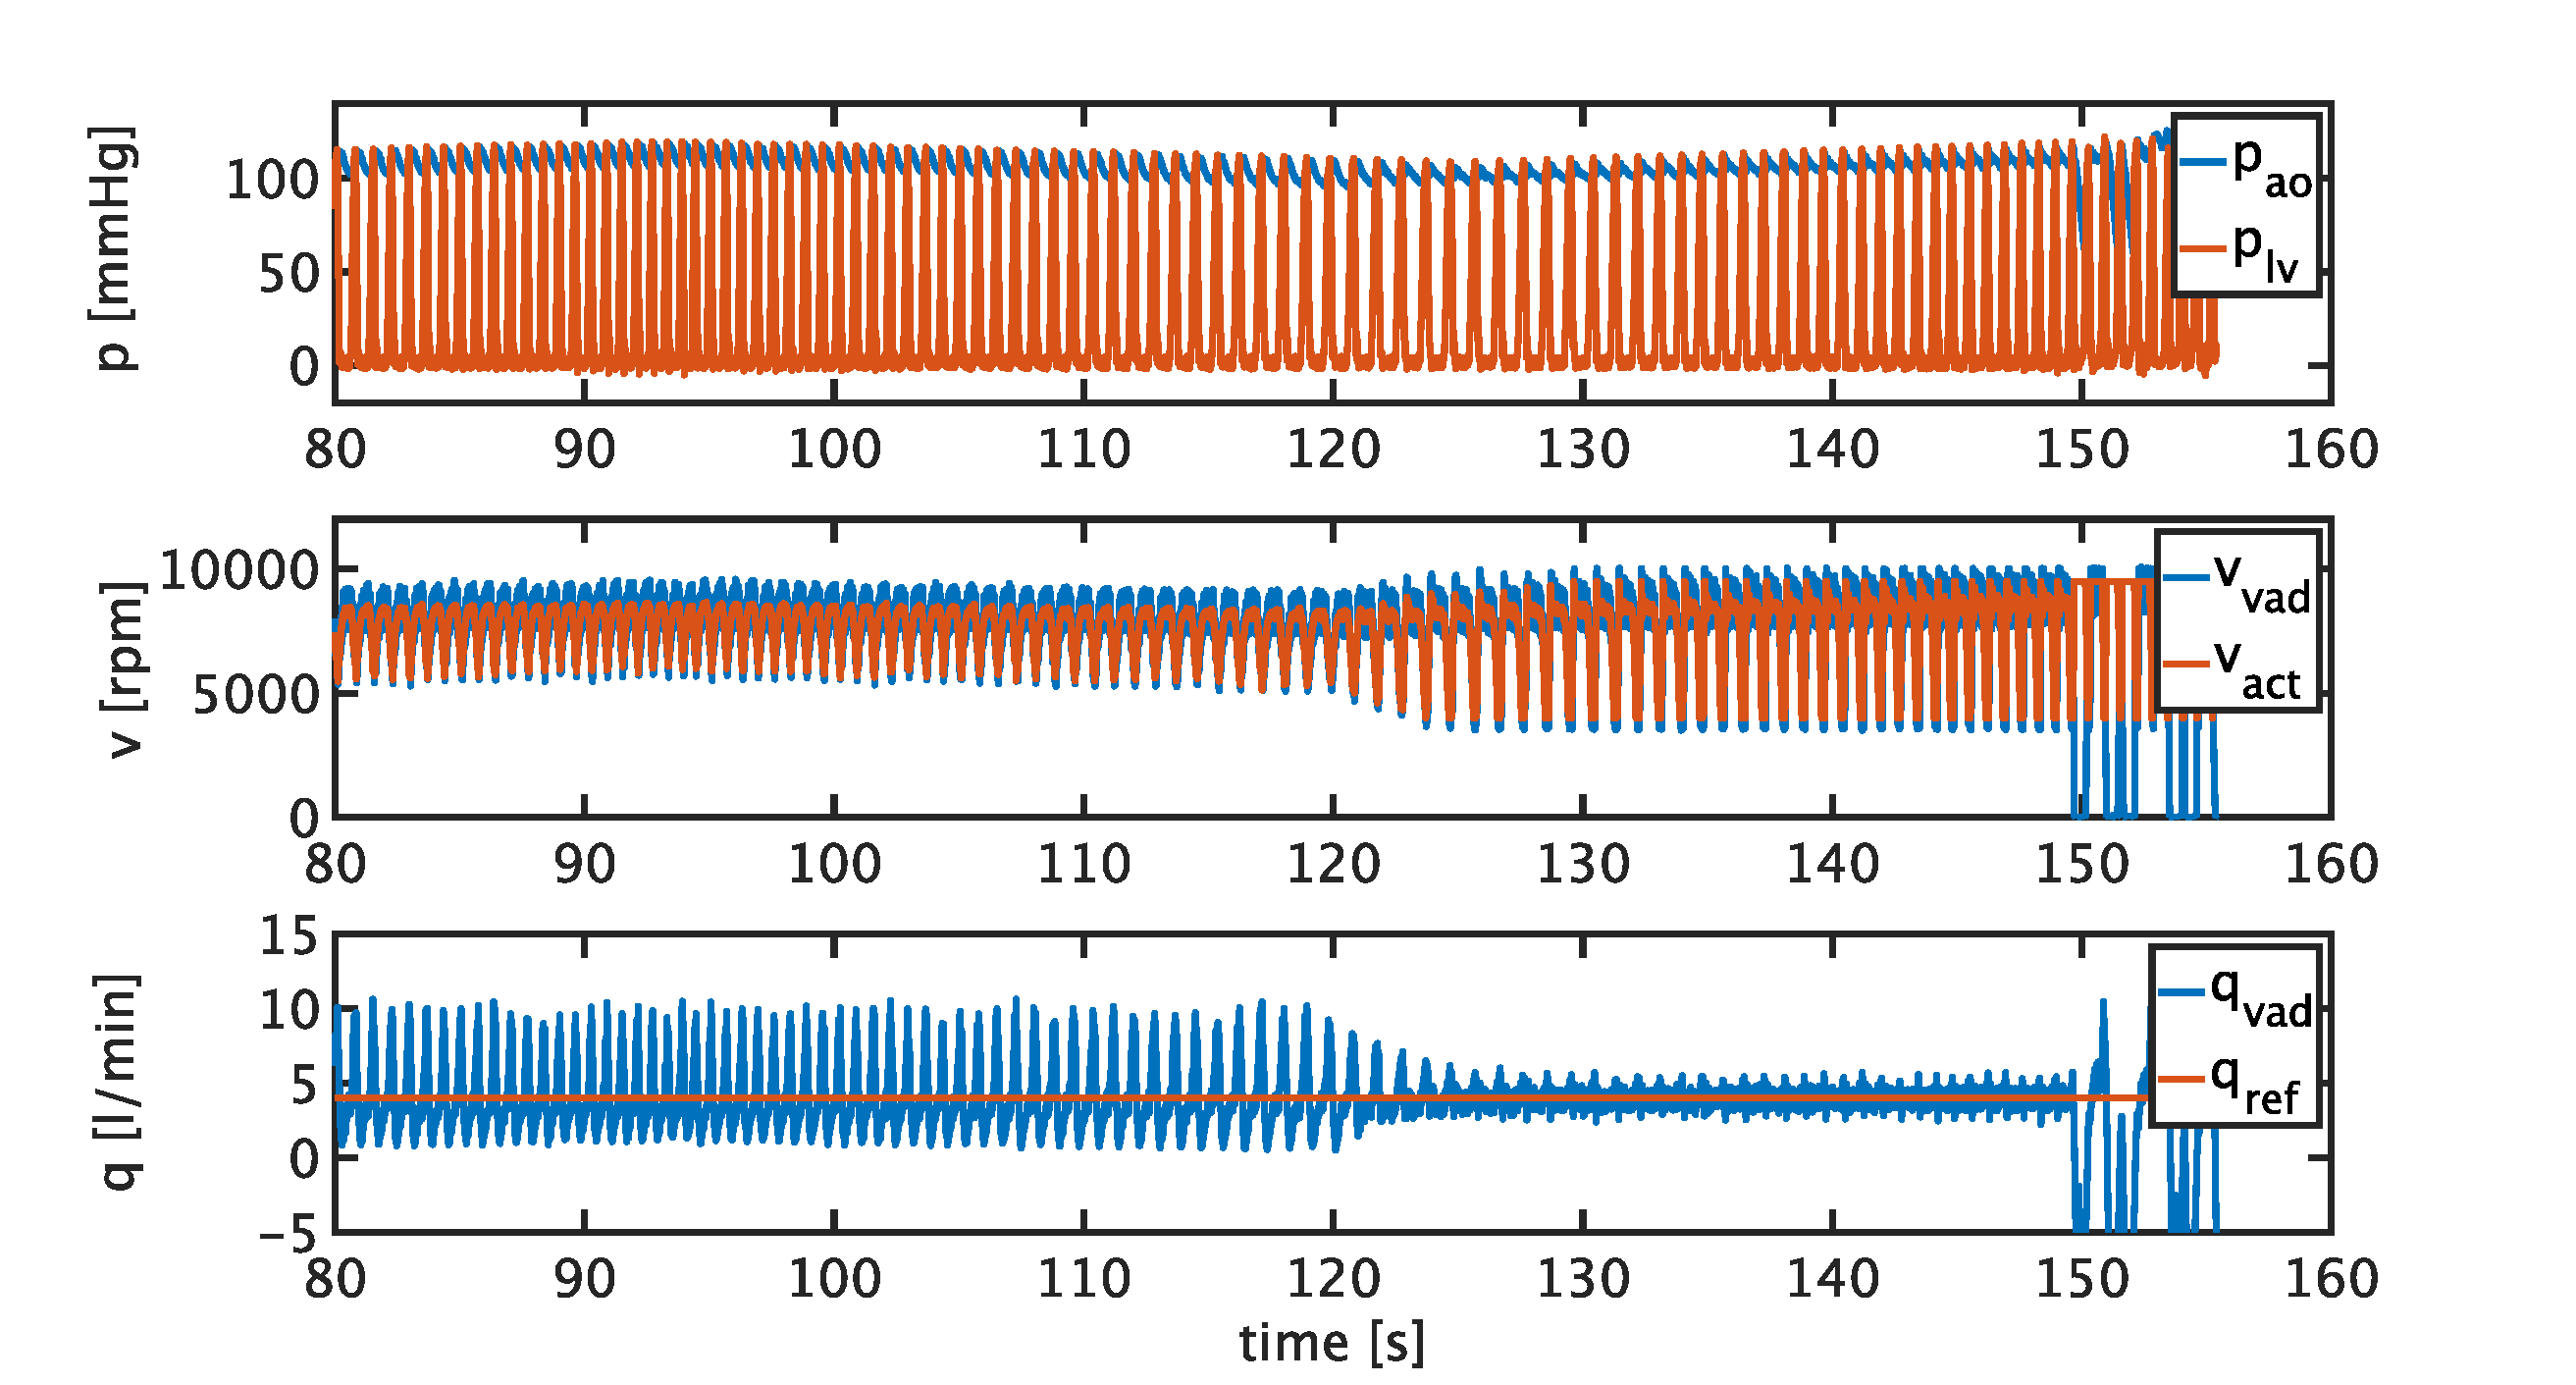
\includegraphics[width=0.95\textwidth]{images/chapt_5/ILC/ilc_var_dist_fix_const.pdf}
  \caption[Segment of measurement for ILC with varying disturbance with $cf_{\mathrm{Lv}}=1$ for constant reference flow with data resampling]{Segment of measurement for ILC with varying disturbance with $cf_{\mathrm{Lv}}=1$ for constant reference flow with data resampling. Top:  pressure values of the MCL. Middle: actuating variable and measured rotational speed of the VAD. Bottom: targeted flow trajectory and measured flow through the VAD}
  \label{fig:ilc_var_dist_fix_const}
\end{figure}
This assumption can be confirmed when comparing the RMSE values of the two measurements.
While at the beginning of combined control both measurements decrease to an average error value of
\begin{equation}
  RMSE_{\mathrm{const,low}}=RMSE_{\mathrm{resampled,const}}\approx0.05\,l/min
\end{equation}
 the value of the measurement without resampling the data afterwards increases continuously to a value of
\begin{equation}
  RMSE_{\mathrm{const,high}}\approx1.13\,l/min.
\end{equation}
The value of the measurement with resampled data remains at about $0.05\,l/min$. Thus, for a constant reference flow, a significant improvement in performance can be achieved by resampling the data of the actuating variable before the output to the control loop.
\figurename~\ref{fig:RMSE_ilc_var_dist_comp_const} depicts a graphical comparison of the RMSE courses of the two measurements.
\begin{figure}[ht!]
  \centering
  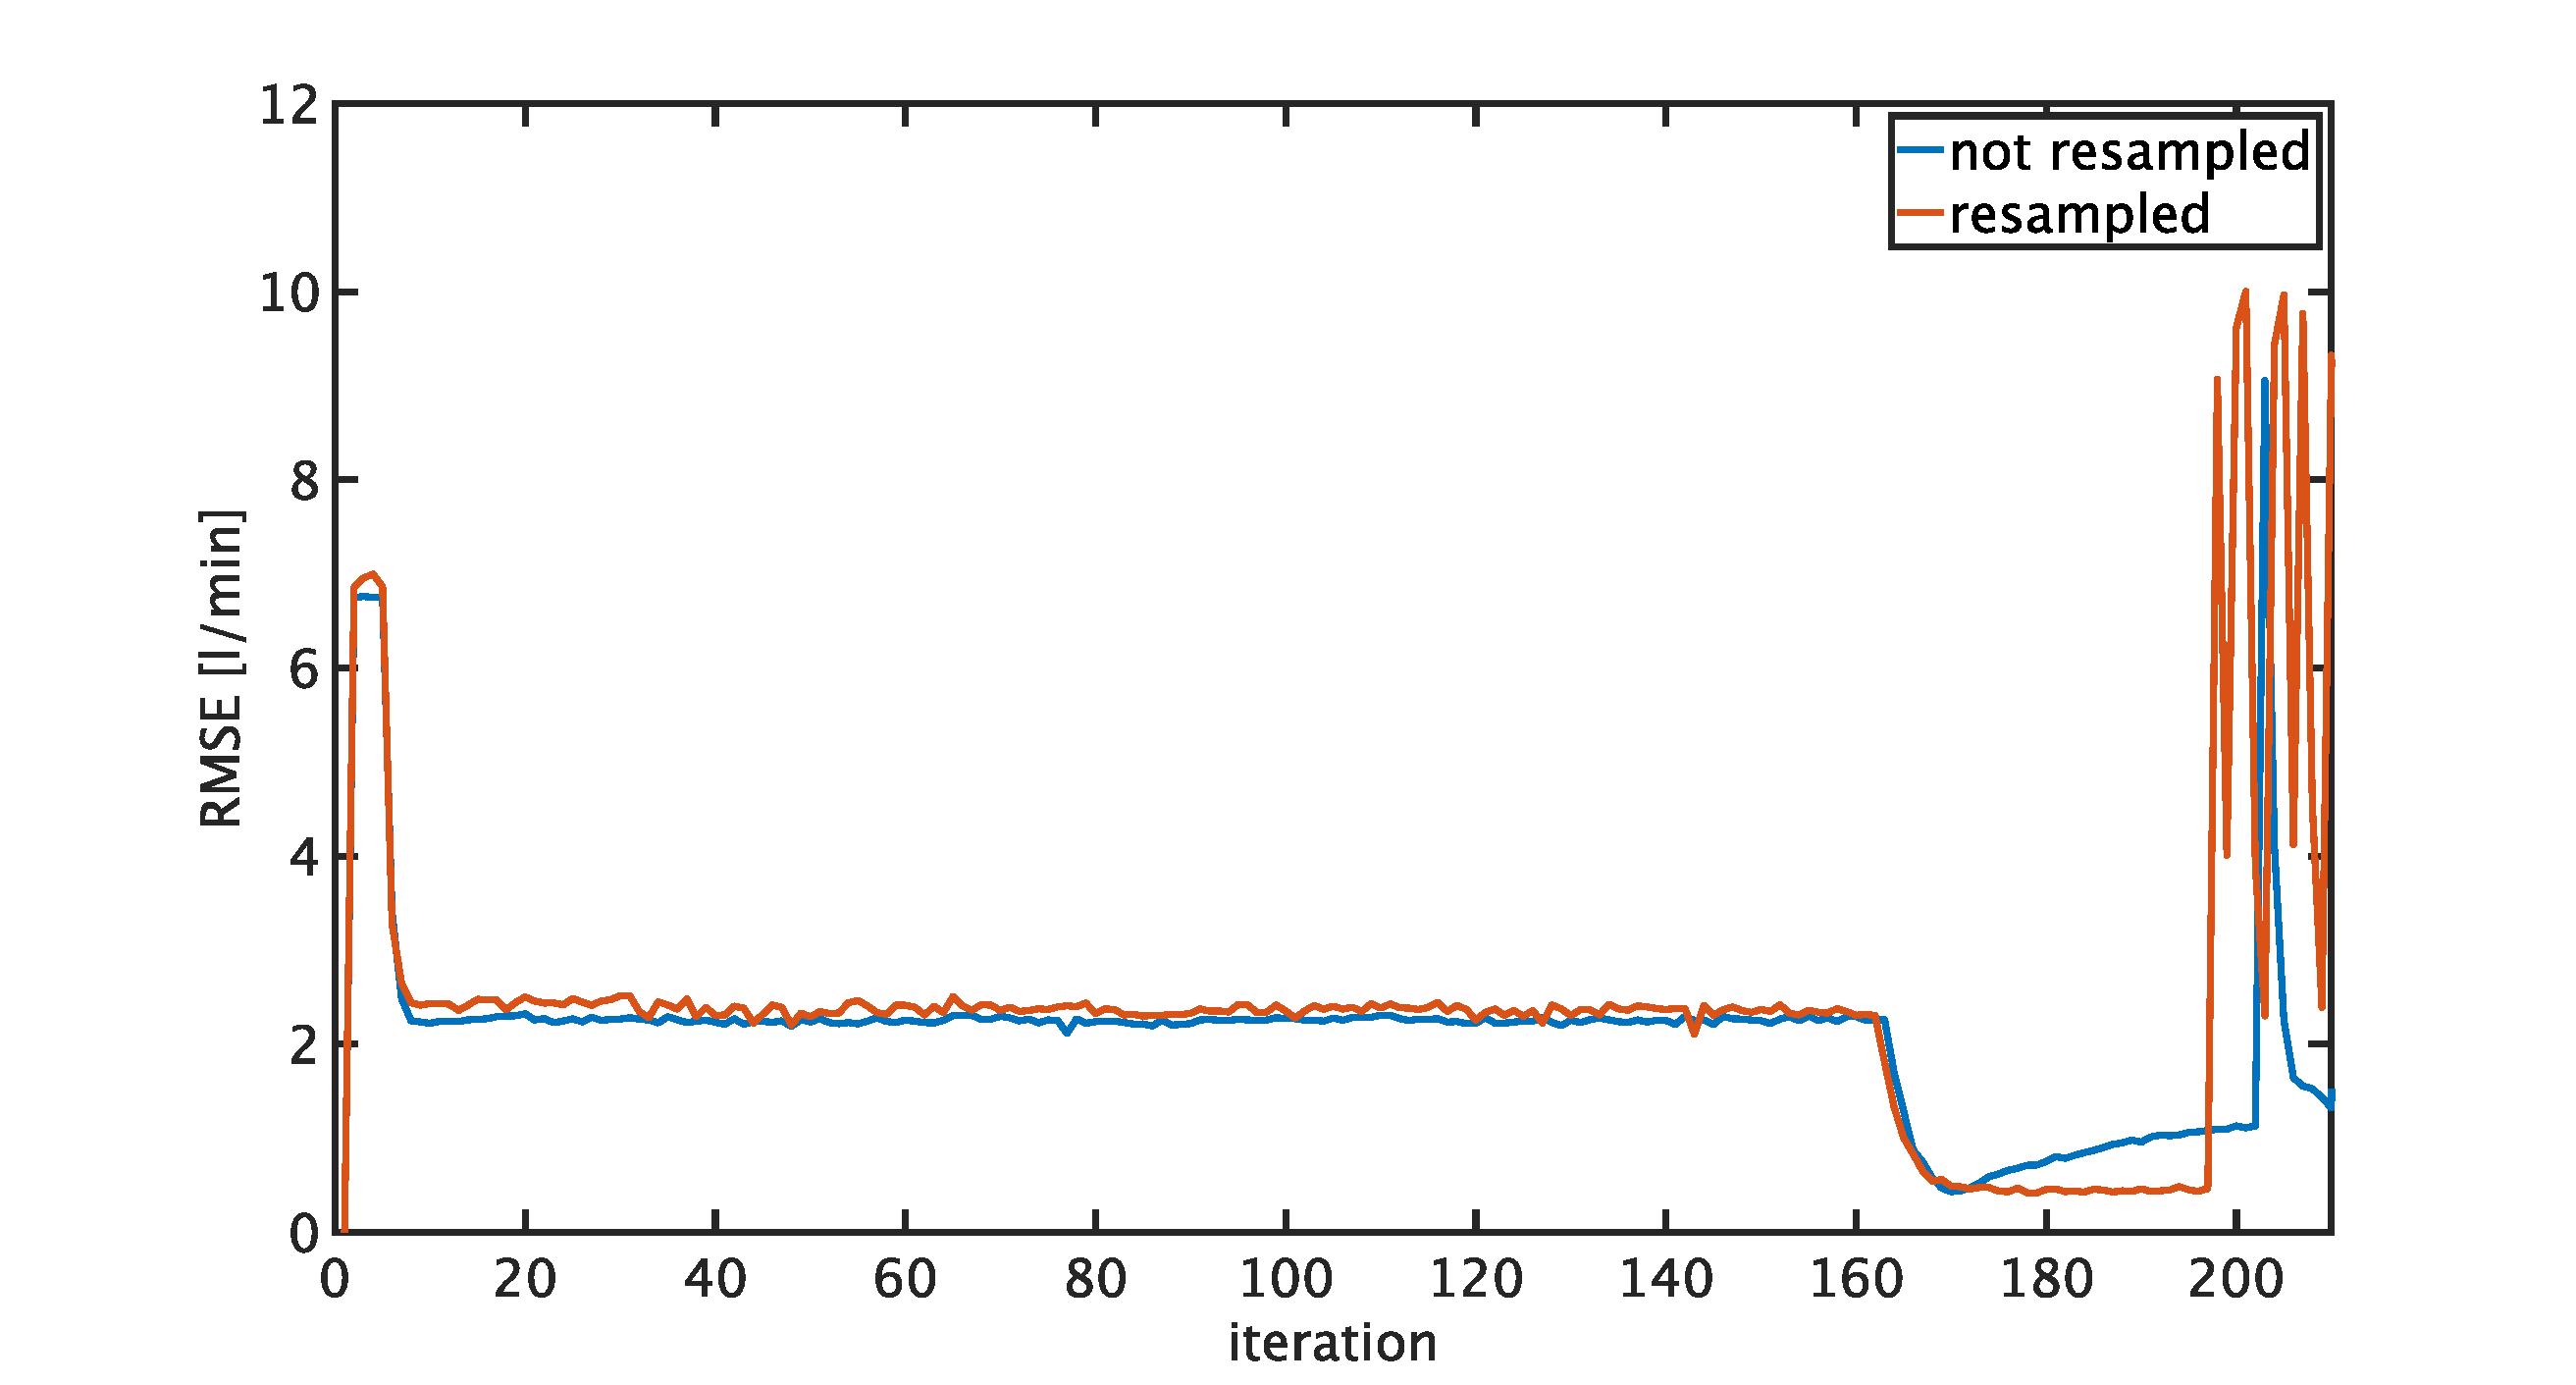
\includegraphics[width=0.95\textwidth]{images/chapt_5/ILC/RMSE_ilc_var_dist_comp_const.pdf}
  \caption[Comparison of RMSE values for ILC measurement using a constant reference flow for unchanged and resampled data]{Comparison of RMSE values for ILC measurement using a constant reference flow for unchanged and resampled data.}
  \label{fig:RMSE_ilc_var_dist_comp_const}
\end{figure}


The second set of measurements is performed using the sinusoidal reference signal. Other than for the constant reference flow for which both the unchanged ILC and the resampling measurement result in a pump failure after approximately $155\,s$, the measurements following a sinusoidal trajectory run stable over the full measurement time of $600\,s$.
Looking at the graphical comparison of the RMSE values of the two measurements, which is shown in \figurename~\ref{fig:RMSE_ilc_var_dist_comp_sine}, significantly lower error values can be seen for the complete measurement period in the measurement using the resampling functionality. For this, the RMSE is about
\begin{equation}
RMSE_{\mathrm{resampled,sine}}\approx0.3\,l/min
\end{equation}
from the onset of the ILC. For the measurement with the standard P-type ILC, permanent fluctuations of the RMSE between
\begin{equation}
 RMSE_{\mathrm{sine,low}}\approx0.3\,l/min
\end{equation}
and
\begin{equation}
 RMSE_{\mathrm{sine,high}}\approx0.9\,l/min
\end{equation}
can be seen.
Thus, an increased performance of the revised ILC can also be concluded for this reference trajectory.
\begin{figure}[ht!]
  \centering
  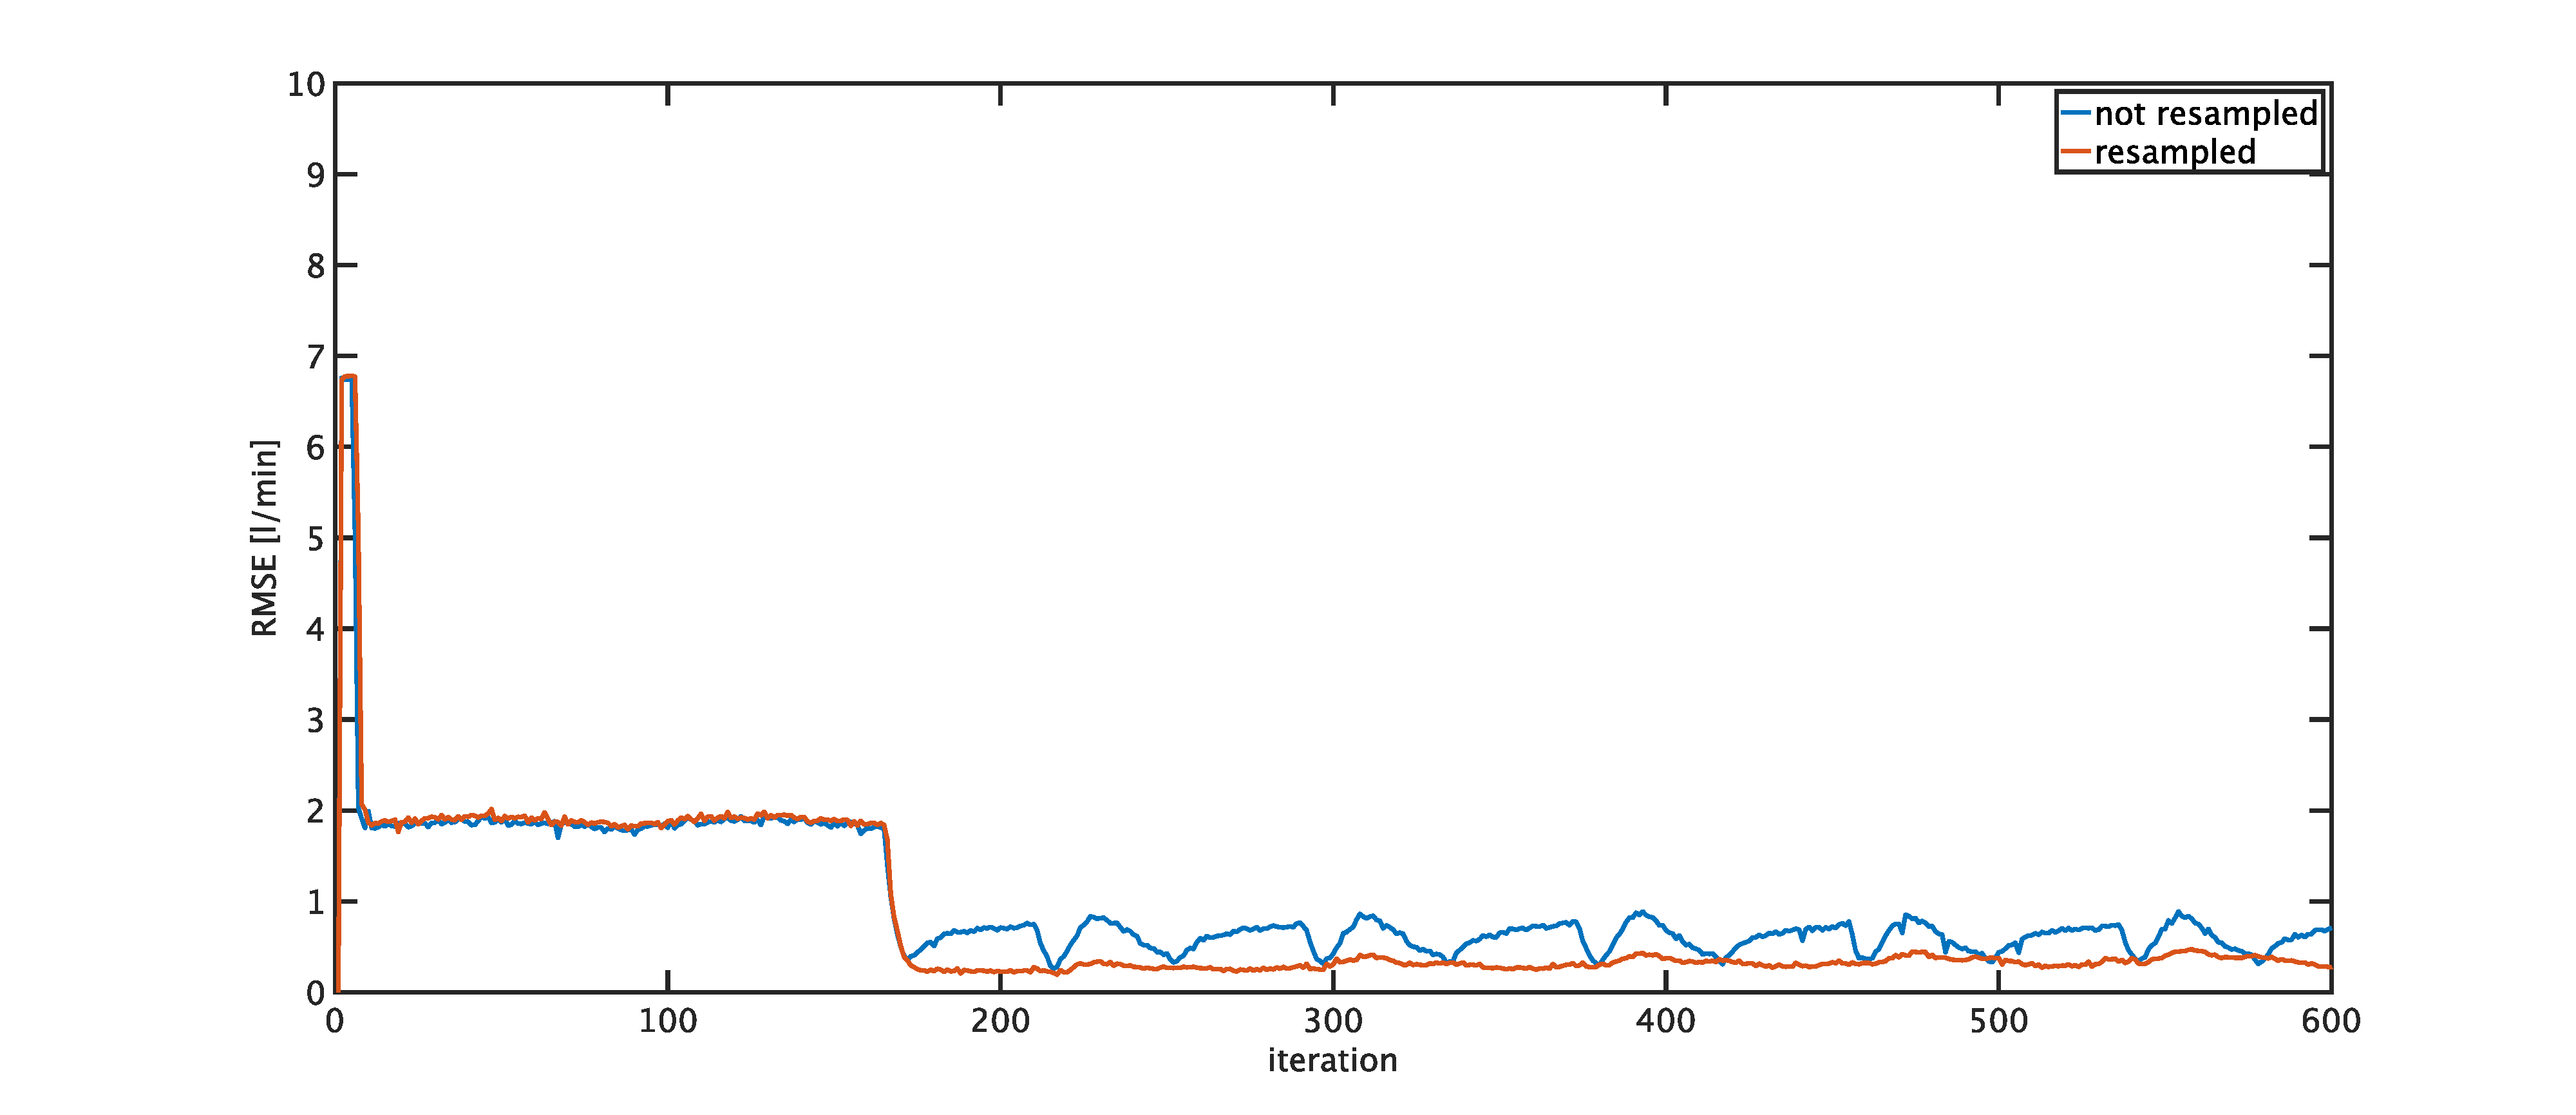
\includegraphics[width=0.95\textwidth]{images/chapt_5/ILC/RMSE_ilc_var_dist_comp_sine.pdf}
  \caption[Comparison of RMSE values for ILC measurement using a sinusoidal reference flow for unchanged and resampled data]{Comparison of RMSE values for ILC measurement using a sinusoidal reference flow for unchanged and resampled data.}
  \label{fig:RMSE_ilc_var_dist_comp_sine}
\end{figure}

The measurements using the triangular reference trajectory show very similar system behavior to those using the constant reference flow.
Both when using the standard ILC and the revised ILC, the pump stops due to oscillating system behavior. This occurs slightly earlier for the measurement using the revised ILC than for the standard ILC. However, when comparing the RMSE values in \figurename~\ref{fig:RMSE_ilc_var_dist_comp_triang} it is clear that the performance of the revised ILC exceeds that of the unmodified ILC. While the revised ILC has average error values of about
\begin{equation}
  RMSE_{\mathrm{resampled,triang}}\approx0.38\,l/min,
\end{equation}
the value for the standard ILC initially drops to about
\begin{equation}
  RMSE_{\mathrm{triang,low}}\approx0.46\,l/min
\end{equation}
but then rises continuously to a value of
\begin{equation}
  RMSE_{\mathrm{triang,high}}\approx0.79\,l/min.
\end{equation}
Thus, even though the pump stops earlier, the use of the revised ILC would be advisable.

\begin{figure}[ht!]
  \centering
  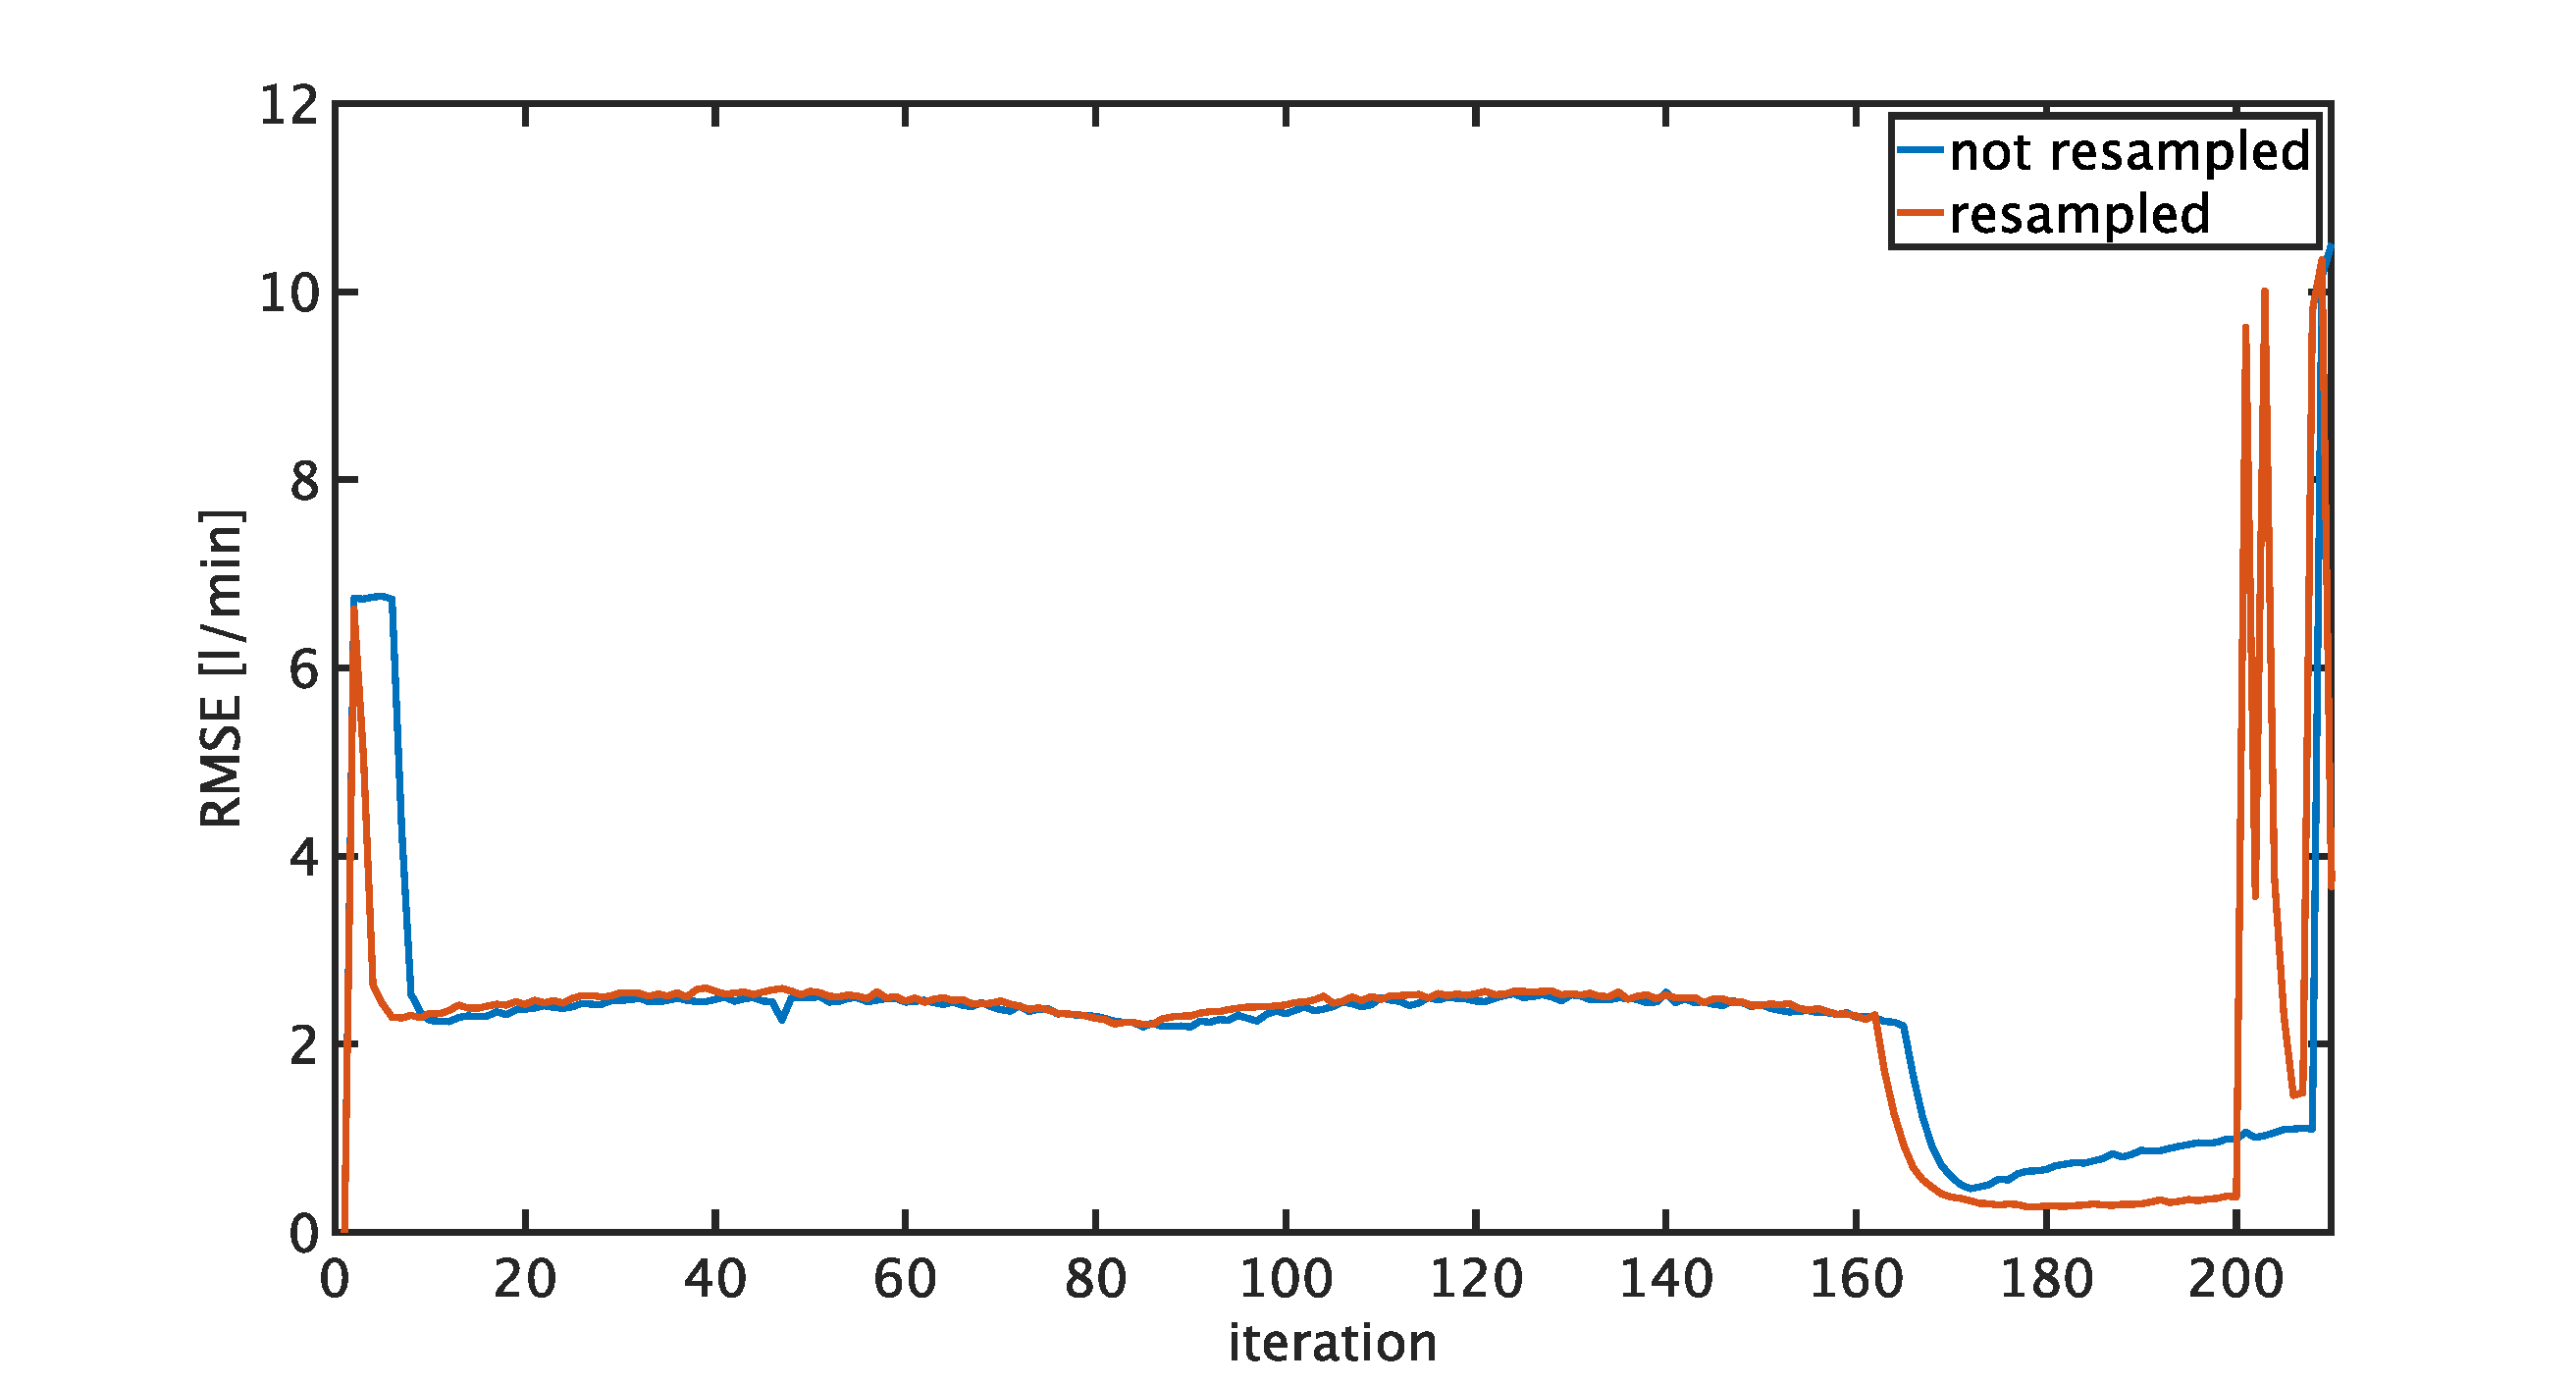
\includegraphics[width=0.95\textwidth]{images/chapt_5/ILC/RMSE_ilc_var_dist_comp_triang.pdf}
  \caption[Comparison of RMSE values for ILC measurement using a triangular reference flow for unchanged and resampled data]{Comparison of RMSE values for ILC measurement using a triangular reference flow for unchanged and resampled data.}
  \label{fig:RMSE_ilc_var_dist_comp_triang}
\end{figure}


Lastly, the tests of the two ILC implementations are performed using the rectangular reference trajectory.  As with the constant reference flow and the triangular trajectory, the actuating variable again oscillates, resulting in the pump rotor stopping.
Unlike the previous measurements, however, the evaluation of the error values for both measurements is similar in this case. At the beginning of the combined control, the averaged error values for both tests drop sharply compared to the PI control. However, a fluctuation of the average error values can be observed for both measurements. This occurs somewhat more slowly for the revised ILC than for the standard ILC. Nevertheless, both measurements show best case values of about
\begin{equation}
  RMSE_{\mathrm{resampled,rect,low}}=RMSE_{\mathrm{rect,low}}\approx0.4\,l/min,
\end{equation}
and worst case values of about
\begin{equation}
  RMSE_{\mathrm{resampled,rect,high}}=RMSE_{\mathrm{rect,high}}\approx0.77\,l/min.
\end{equation}
A graphical comparison is presented in \figurename~\ref{fig:RMSE_ilc_var_dist_comp_rect}.
\begin{figure}[ht!]
  \centering
  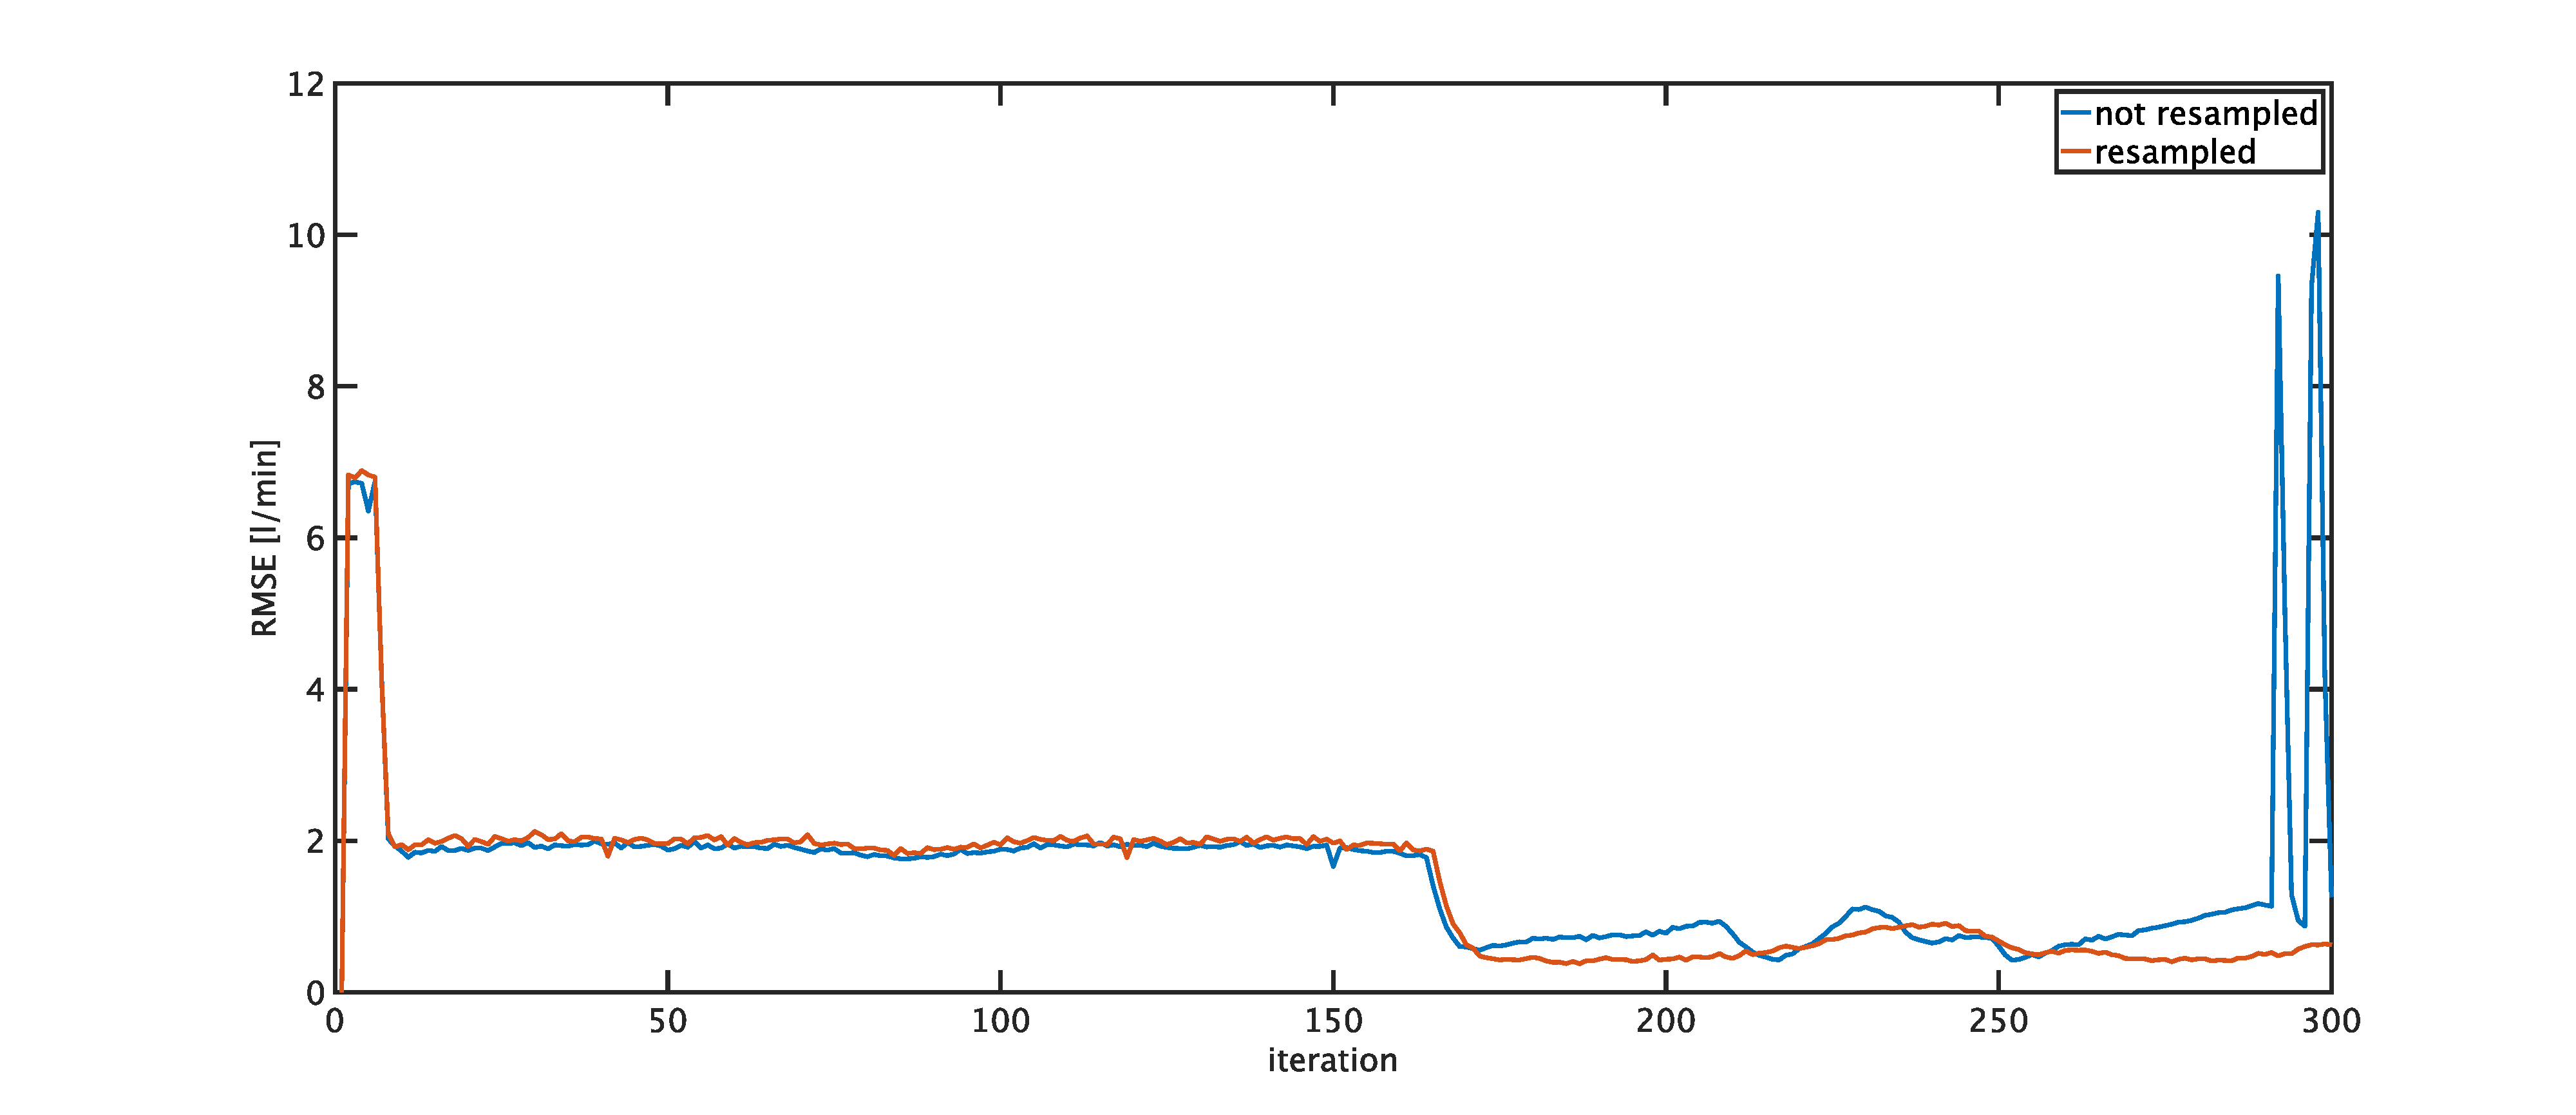
\includegraphics[width=0.95\textwidth]{images/chapt_5/ILC/RMSE_ilc_var_dist_comp_rect.pdf}
  \caption[Comparison of RMSE values for ILC measurement using a rectangular reference flow for unchanged and resampled data]{Comparison of RMSE values for ILC measurement using a rectangular reference flow for unchanged and resampled data.}
  \label{fig:RMSE_ilc_var_dist_comp_rect}
\end{figure}
Due to this perception, no clear statement can be made for the reference tracking of this trajectory as to which of the ILC approaches is more suited.
\\Graphical representations of the transitional segments for the performed measurements using sinusoidal, triangular and rectangular reference trajectories can be found in \figurename~\ref{fig:anh_9} to \figurename~\ref{fig:anh_14} of the appendix.

\tablename~\ref{tab:compare_ILC} depicts an overview on the worst case RMSE values of the standard ILC and the RMSE values for the revised ILC for all reference trajectories. It furthermore gives the difference between these error values as $\Delta{RMSE}$.
\begin{table}[h]
  \centering
  \begin{tabular}{c|c|c|c}
    \toprule
     reference trajectory & $RMSE_{\mathrm{std\_ILC,high}}$ & $RMSE_{\mathrm{resampled}} $ & $\Delta{RMSE} $\\
     & $[l/min]$ & $[l/min]$ & $[l/min]$\\
    \midrule
    constant flow & $1.13$ & $0.05$ & $1.08$ \\
    sinusoidal & $0.9$ & $0.3$ & $0.6$ \\
    triangular & $0.79$ & $0.38$ & $0.41$ \\
    rectangular & $0.77$ & $0.77$ & - \\
    \bottomrule
\end{tabular}
  \caption[RMSE values for different reference trajectories of standard ILC and revised ILC]{RMSE values for different reference trajectories of standard ILC and revised ILC.}
  \label{tab:compare_ILC}
\end{table}
\\The highest improvement is achieved for the constant reference flow with $\Delta{RMSE}=1.08\,l/min$. Also for constant reference flow the highest overall performance is achieved with an RMSE of only $0.05\,l/min$. This can be explained by the fact that the length of the reference signal does not change for a constant flow, while this is the case for all other signals.
